%===================================================================================================
% Radiotechnika
% RA.tex
%===================================================================================================
% notes:
%~~~~~~~~~
%---------------------------------------------------------------------------------------------------
% Setting path to image 
  \graphicspath{{../src/RAE/img/}}

%---------------------------------------------------------------------------------------------------
%                               RAE
%---------------------------------------------------------------------------------------------------
\LuaPartBckgrnd{titleBG_fractal1.png}
\LuaPartTitle{VFT}{Radioelektronika}{VFT}
\parttoc

\ifthenelse{ \equal{\DebugMode}{true} }{
% Debug mode ON
  % % !TeX spellcheck = cs_CZ
\sisetup{input-complex-roots = j, 
         output-complex-root = \ensuremath{\mathrm{j}}}
         
%==================Kapitola: Teoretické základy radioelektroniky====================================
\chapter{Teoretické základy radioelektroniky}\label{chap:ra_theory}
\minitoc
  %--------------- Úvod do šíření vln pro pozemní rádiové spoje ------------------------------------
  \section{Úvod do šíření vln pro pozemní rádiové spoje}
    \begin{example}
      Domácí meteostanice používá pro komunikaci s externím čidlem na měření vnější teploty 
      frekvenci \SI{433}{MHz}. Určete délku vln a rádiové pásmo do kterého použitá vlnová délka 
      patří.
      \newline\textbf{řešení:}
      \begin{equation}
        \lambda = c\cdot T = \frac{c}{f} = \frac{\num{300e6}}{\num{433e6}} = \SI{0.49}{\meter}
      \end{equation}
      Domácí meteostanice používá pro komunikaci s čidlem ultrakrátké vlny o vlnové délce 
      \SI{0.49}{\meter} 
    \end{example}
    
  %--------------- Základní klasifikace radioelektronických systémů --------------------------------
  \section{Základní klasifikace radioelektronických systémů}
    Pod pojmem systém \cite[s.~56]{ZaludRA} 

  \section{Dvojbrany v radioelektronice}
    Pod pojmem \emph{systém} se zde označuje elektrický obvod nebo soustava obvodů, které vytvářejí 
    alespoň jeden výstupní signál jako odezvu na alespoň jeden vstupní signál. Jednou z 
    nejdůležitějších tříd radioelektronických systémů jsou lineární systémy s časově invariantními 
    (neměnnými) parametry, které mají podobu \emph{n-branů}. Mezi nimi potom zaujímají významné 
    místo lineární dvojbrany a trojbrany, jejichž popisem a obecnými vlastnostmi se zabývá tato 
    kapitola. Připomeňme, že pro označení linearity a časové invariance se v teorii obvodů používá 
    zkratka \emph{LTI- (Linear Time Invariant)}, což nijak dále nezdůrazňujeme, nebo tato kapitola 
    je zaměřena právě jen na dvojbrany a trojbrany tohoto typu.
    
    V radioelektronice se často vyskytují dvojbrany a trojbrany, které přísně vzato lineární 
    nejsou, avšak jejich nelinearity jsou tak malé, že je lze v technické praxi zanedbat; do této 
    kategorie patří například všechny obvody s diodami a s tranzistory, pracujícími v režimu malých 
    signálů, kde jsou prakticky lineární a nelinearity se u nich začínají projevovat až při vyšších 
    úrovních signálů. Tyto dvojbrany a trojbrany, označované termínem kvazilineární (tedy téměř 
    lineární) Jsou rovněž zahrnuty do této kapitoly. Zvláštní pozornost je věnována zejména jejich 
    vlastnostem v hraniční oblasti mezi lineárním a nelineárním režimem, která je v 
    radioelektronice velmi důležitá.
    
    \subsection{Admitanční parametry a rozptylové parametry dvojbranů}
      Pod pojmem dvojbran (\emph{two-port}) se rozumí elektrický systém, který má jeden pár 
      vstupních svorek a jeden pár výstupních svorek, tedy jednu vstupní a jednu výstupní bránu 
      (dvojbran zřejmě představuje zvláštní třídu obecnějšího pojmu \emph{čtyřpól}, který má čtyři 
      nezávislé svorky). Linearizované přenosové vlastnosti dvojbranů je možné charakterizovat 
      pomocí jejich \textbf{admitančních} a \textbf{rozptylových parametrů}, kterým je dále 
      věnována náležitá pozornost \cite[s.~331]{ZaludRA}.
      
      Při definici \emph{admitančních parametrů} dvojbranů, nazývaných také parametry \(y\) 
      \emph{(Admittance Parameters)}, vyjdeme z obr. \ref{RA:fig_dvojbran01}. Zde je znázorněn 
      lineární časově invariantní dvojbran, který má na vstupu svorkové napětí a proud \(u_l\), 
      \(i_1\) a na výstupu \(u_2\), \(i_2\). K jeho vstupu je připojen generátor s vnitřní 
      admitancí \(Y_g\) a k výstupu zatěžovací admitance \(Y_z\). Admitanční parametry tohoto 
      dvojbranů jsou definovány relacemi
      \begin{align}
        i_1 &= y_{11}u_1 + y_{12}u_2   \\ 
        i_2 &= y_{21}u_1 + y_{22}u_2
      \end{align}
      
      \begin{figure}[ht!]
        \centering  
        \begin{tabular}{cc}
          \subfloat[ ]{\label{RA:fig_dvojbran01}
            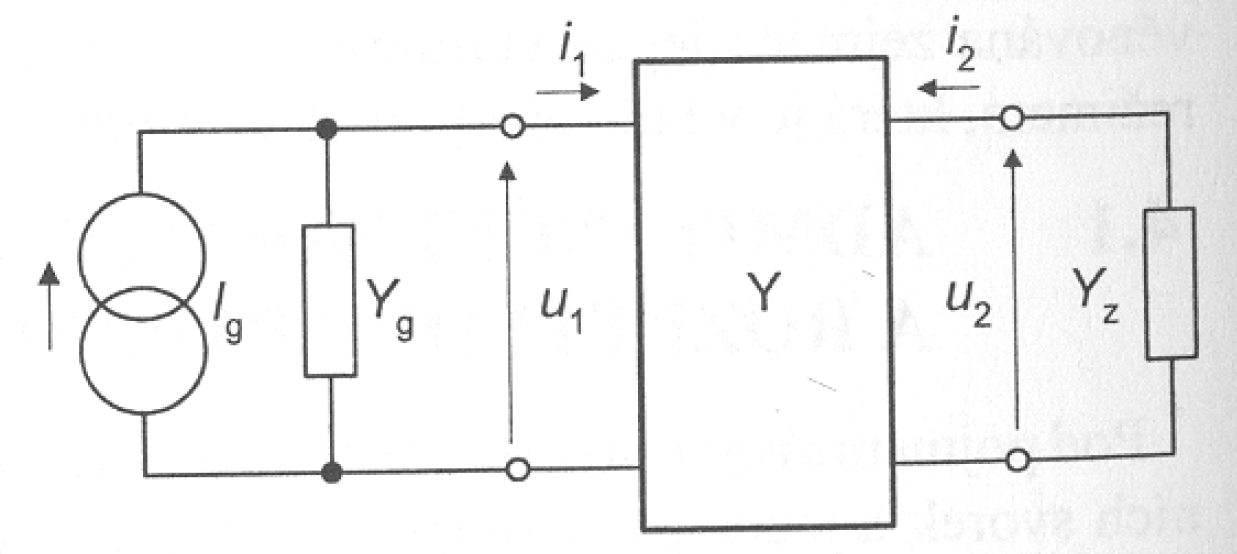
\includegraphics[width=0.4\linewidth]{RA_dvojbran01.png}}              &
          \subfloat[ ]{\label{RA:fig_dvojbran02}
            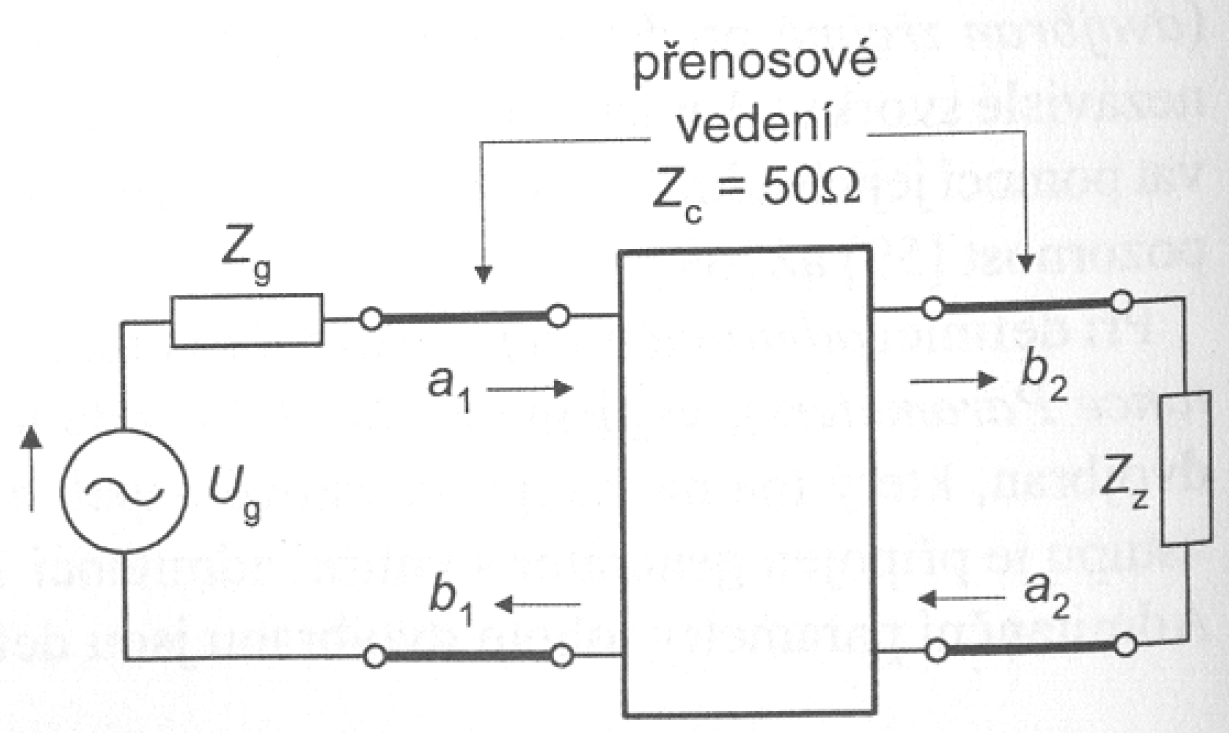
\includegraphics[width=0.4\linewidth]{RA_dvojbran02.png}}              \\
        \end{tabular}
        \caption{Charakterizace dvojbranu: a) svorkovými napětími a proudy; 
                 b) dopadajícímí a odraženými napěťovými vlnami}\label{RA:fig_dvojbran}
      \end{figure}
      
      Z těchto vztahů vyplývá, že admitance \(y_{11}\) je rovna \emph{vstupní admitanci dvojbranu} 
      při jeho výstupu nakrátko (\(u_2=0\)), a podobně admitance \(y_{22}\) je \emph{výstupní 
      admitance} při vstupu nakrátko (\(u_1=0\)). Admitance \(y_{21}\), resp. \(y_{12}\) je potom 
      \emph{přenosová admitance} v předním nebo zpětném směru, při výstupu resp. vstupu nakrátko.
      
      Jak je patrné, parametry \(y\) jsou definovány při vstupu nebo výstupu nakrátko. Při jejich 
      měření však lze tuto podmínku splnit bez potíží jen při nižších kmitočtech, nepřesahujících 
      asi 300 MHz. Ve vyšších pásmech je možné vytvořit „zkrat“ např. vyladěným sériovým 
      rezonančním obvodem, nebo transformačním členem složeným z obvodů s rozloženými parametry, 
      což však příliš komplikuje měření (velké potíže vznikají zejména při návrhu širokopásmových 
      automatizovaných měřičů parametrů \(y\) s rozmítaným kmitočtem, které jsou v mikrovlnném 
      pásmu prakticky nerealizovatelné). Z tohoto, ale i z dalších důvodů byla během šedesátých let 
      propracována nová soustava parametrů označovaných jako parametry \(s\), nebo 
      \textbf{parametry rozptylové} (\emph{Scattering Parameters}). Definice rozptylových parametrů 
      dvojbranů vychází z obr. \ref{RA:fig_dvojbran02}. Zde je opět znázorněn lineární, časově 
      invariantní dvojbran, avšak jeho vlastnosti již nejsou charakterizovány svorkovými napětími a 
      proudy, ale \emph{normovanými dopadajícími napěťovými vlnami} \(a_1, a_2\) a \emph{odraženými 
      napěťovými vlnami} \(b_1, b_2\). Tyto vlny se vytvářejí na vstupním a na výstupním přenosovém 
      vedení o charakteristické impedanci \(Z_c\). Svorková napětí a proudy jsou vázány s 
      napěťovými vlnami jednoduchými vztahy
      \begin{align}\label{RA:eq_01}
      u_1 &= (a_1 + b_1)\cdot\sqrt{Z_c} \qquad i_1 = \frac{a_1-b_1}{\sqrt{Z_c}}   \\ 
      u_2 &= (a_2 + b_2)\cdot\sqrt{Z_c} \qquad i_1 = \frac{a_2-b_2}{\sqrt{Z_c}}
      \end{align}
      
      Naopak dopadající a odražené vlny jsou v závislosti na svorkových napětích a proudech určeny 
      vztahy
      \begin{align}\label{RA:eq_02}
      a_1 &= \frac{u_1 + i_1Z_c}{2\sqrt{Z_c}} \qquad b_1 = \frac{u_1 - i_1Z_c}{2\sqrt{Z_c}}   \\ 
      a_2 &= \frac{u_2 + i_2Z_c}{2\sqrt{Z_c}} \qquad b_1 = \frac{u_2 - i_2Z_c}{2\sqrt{Z_c}}
      \end{align}
      
      \emph{Charakteristická impedance} \(Z_c\), nazývaná v této souvislosti také \emph{impedancí 
      vztažnou (referenční)}, může obecně být komplexní veličinou; dále však předpokládejme, že je 
      reálná, stejná pro vstupní i výstupní bránu, s typickou hodnotou \(Z_c = \SI{50}{\ohm}\) (v 
      praxi se používají ještě impedance \SI{60}{\ohm} a \SI{75}{\ohm}). Vzájemnou závislost 
      dopadajících a odražených napěťových vln vyjadřují relace
      \begin{align}\label{RA:eq_03}
      b_1 &= s_{11}a_1 + s_{12}a_2   \\ 
      b_2 &= s_{21}a_1 + s_{22}a_2
      \end{align}
      které lze považovat za definiční vztahy rozptylových parametrů daného dvojbranu. Z nich se 
      snadno odvodí fyzikální význam jednotlivých parametrů:
      \begin{itemize}
        \item \textbf{vstupní napěťový činitel odrazu}, při výstupu zakončeném zátěží \(Z_z\), 
              přizpůsobenou k vztažné impedanci \(Z_c\)  (tj. \(Z_z = Z_c\) a tedy \(a_2 = 0\)):
              \begin{equation*}
                s_{11} = \left(\dfrac{b_1}{a_1}\right)_{a_2=0}
              \end{equation*}
        \item \textbf{výstupní napěťový činitel odrazu}, při vstupu zakončeném impedancí \(Z_g\), 
               přizpůsobenou k vztažné impedanci \(Z_c\) (tj. \(Z_g = Z_c\) a tedy \(a_1 = 0\)); 
              \begin{equation*}
                 s_{22} = \left(\dfrac{b_2}{a_2}\right)_{a_1=0}
              \end{equation*}
        \item \textbf{vložné napěťové zesílení v předním směru}, při výstupu zakončeném zátěží 
              \(Z_z\), přizpůsobenou k vztažné impedanci \(Z_c\) (tj. \(Z_z = Z_c\) a tedy \(a_2 = 
              0\));
              \begin{equation*}
                 s_{12} = \left(\dfrac{b_1}{a_2}\right)_{a_1=0}
              \end{equation*}
        \item \textbf{vložné napěťové zesílení v závěrném směru}, při vstupu zakončeném impedancí 
              \(Z_g\), přizpůsobenou k vztažné impedanci \(Z_c\) (tj.\(Z_g = Z_c\) a tedy \(a_1 = 
              0\)); \\
              \begin{equation*}
                 s_{12} = \left(\dfrac{b_1}{a_2}\right)_{a_1=0}
              \end{equation*}
      \end{itemize}
      
      Takto definované parametry \(s\) jsou závislé na impedanci \(Z_c\), proto jejich číselné 
      hodnoty je třeba vždy doplnit údajem o její hodnotě. Při grafickém znázornění se parametry 
      \(s_{11}\) a \(s_{22}\), představující \emph{činitele odrazu}, zakreslují obvykle do 
      příslušného rastru \emph{Smithova diagramu}; parametry \(s_{12}\) a \(s_{21}\) se potom 
      zobrazují do komplexní roviny, nejčastěji v polárním tvaru.
        
      V předchozích úvahách jsou rozptylové parametry definovány pomocí normovaných napěťových vln 
      \(a\), \(b\). Kvadráty modulů těchto vln \(a_2\) resp. \(b_2\) jsou rovny dopadajícím resp. 
      odraženým výkonům na vstupu a na výstupu dvojbranu. Proto se vlny \(a\), \(b\) označují také 
      jako výkonové vlny, ačkoliv přesněji vzato vyjadřují odmocniny z příslušných výkonů.
        
      Nehledě na to, že parametry \(y\) jsou definovány pomocí svorkových napětí a proudů a 
      parametry \(s\) pomocí dopadajících a odražených vln, existují mezi nimi vzájemné jednoznačné 
      vztahy. Tak např. parametr \(y_{11}\) definovaný pro \(u_2 = 0\), tj. pro 
      \(\dfrac{a_2}{b_2}=-1\), lze se zřetelem na převodní vztahy (\ref{RA:eq_01}), 
      (\ref{RA:eq_02}) vyjádřit ve tvaru
      \begin{equation}\label{RA:eq_04}
        y_{11} = \left(\frac{i_1}{u_1}\right)_{u_{22}} = \frac{a_1-b_1}{Z_c(a_1+b_1)} = 
                 \frac{1-\dfrac{b_1}{a_1}}{Z_c1+\left(\dfrac{b_1}{a_1}\right)} 
      \end{equation}
      Z definičních vztahů (\ref{RA:eq_03}) však plyne, že \(\frac{b_1}{a_1} = (\det s + s_{11})(1 
      + s_{22})\), kde \(\det s = s_{11}s_{22} -s_{21}s_{l2}\). Dosazením poslední relace do 
      (\ref{RA:eq_04}) se tedy získá převodní vztah
      \begin{equation}
        y_{11} = \frac{(1+s_{22})(1-s_{11})+s_{12}s_{21}}{(1+s_{11})(1+s_{22})-s_{12}s_{21}}
      \end{equation}
      
    \subsection{Vektorové měření impedance a přizpůsobení}
      \subsubsection{Činitel odrazu, přepočet na impedanci, poměr stojatého vlnění}
        Komplexní činitel odrazu \(\Gamma_L\) zátěže o impedanci \(Z_L\) připojené na konec 
        homogenního vedení o vlnové impedanci \(Z_0\) je v rovině připojení impedance \(Z_L\) 
        definován jako poměr fázoru harmonické napěťové vlny \(U^-\) na svorkách zátěže \(Z_L\), 
        která se od této zátěže odráží (odražená vlna), ku fázoru napěťové vlny \(U^+\) na svorkách 
        zátěže \(Z_L\), která na zátěži \(Z_L\) přichází po vedení (postupná vlna), tj.
        \begin{equation}\label{RA:eq_smith01}
          \Gamma_L = \frac{U^-}{U^+}
        \end{equation}
        Činitel odrazu je v této rovině funkcí pouze \(Z_0\) a \(Z_L\), přičemž obě tyto impedance 
        mohou být kmitočtově závislé (a také bývají, zejména \(Z_L\)).
  
        Mezi činitelem odrazu \(\Gamma_L\) a impedancemi \(Z_0\) a \(Z_L\) lze odvodit vztah
        \begin{equation}\label{RA:eq_smith02}
          \Gamma_L = \frac{Z_L-Z_0}{Z_L-Z_0}.
        \end{equation}    
        Pokud známe vlnovou impedanci vedení \(Z_0\) a činitel odrazu \(\Gamma_L\), lze ze vztahu 
        \ref{RA:eq_smith02} snadno vyjádřit zatěžovací impedanci \(Z_L\)
        \begin{equation}\label{RA:eq_smith03}
          Z_L = Z_0\frac{1+\Gamma_L}{1-\Gamma_L},
        \end{equation}    
  
        často udávaným parametrem popisujícím míru nepřizpůsobení je poměr stojatého vlnění – 
        \textbf{PSV} \emph{(Voltage Standing Wave Ratio – VSWR)}. Je definován jako poměr maximální 
        a minimální hodnoty amplitudy tzv. stojatého vlnění, které vzniká součtem postupné a 
        odražené vlny na vedení. Poměr stojatého vlnění lze vyjádřit taktéž pomocí vlnové impedance 
        vedení \(Z_0\) a zatěžovací impedance \(Z_L\), a tedy i pomocí činitele odrazu \(\Gamma_L\)
        \begin{equation}\label{RA:eq_smith04}
          PSV = \frac{U_{max}}{U_{min}} 
              = \frac{\abs{Z_L+Z_0} + \abs{Z_L-Z_0}}{\abs{Z_L+Z_0} - \abs{Z_L-Z_0}} 
              = \frac{1+\abs{\Gamma_L}}{1-\abs{\Gamma_L}}.
        \end{equation}
        Poslední výraz umožňuje odpoutat definici poměru stojatého vlnění od vedení a pracovat s 
        ním podobně jako s velikostí činitele odrazu \(\Gamma_L\).
      
      \subsubsection{Impedanční přizpůsobení pomocí obvodů se soustředěnými parametry}
        Přivádíme-li vysokofrekvenční signál z generátoru o vnitřní impedanci \(Z_G\) na zátěž o 
        impedanci \(Z_L\), je obvykle žádoucí dosažení stavu tzv. \emph{impedančního přizpůsobení}. 
        Přitom rozlišujeme dva typy impedančního přizpůsobení. Prvním je \emph{impedanční 
        přizpůsobení pro maximální přenos výkonu}, pro které platí
        \begin{equation}\label{RA:eq_smith05}
          Z_L = Z^*_G,
        \end{equation}  
        kde \(Z^*_G\) je komplexně sdružená hodnota k vnitřní impedanci generátoru \(Z_G\). V tomto 
        stavu obdržíme na zátěži \(Z_L\) největší činný výkon, jaký je generátor vůbec schopen do 
        nějaké zátěže dodat – tzv. \emph{dosažitelný výkon}.
  
        Druhým typem je \emph{bezodrazové impedanční přizpůsobení}, vhodné v případě, kdy na zátěž 
        \(Z_L\) přivádíme signál po vedení o vlnové impedanci \(Z_0\) nezanedbatelné délky vzhledem 
        k vlnové délce signálu. V tomto stavu platí
        \begin{equation}\label{RA:eq_smith06}
          Z_L = Z_0,
        \end{equation}  
        a jeho výhodou je, že při něm na konci vedení nedochází k odrazům, které by jinak mohly 
        kromě zhoršení účinnosti přenosu výkonu způsobit také degradaci kvality signálu (v případě 
        odrazů na obou koncích vedení, např. tzv. „duchy“ v televizním obrazu způsobené právě 
        nepřizpůsobeným anténním napáječem). Jelikož u většiny vedení máme v praxi téměř nulovou 
        imaginární část vlnové impedance \(Z_0\) (přesně nulovou mají bezeztrátová vedení), je 
        bezodrazové impedanční přizpůsobení obvykle současně přizpůsobením pro maximální přenos 
        výkonu (avšak pouze za předpokladu, že je provedeno na obou koncích vedení, tj. jak na 
        straně zátěže, tak na straně generátoru).
  
        V našem případě budeme bezodrazově přizpůsobovat určitou zatěžovací impedanci \(Z_L\) k 
        vedení o reálné vlnové impedanci \(Z_0 = \SI{50}{\ohm}\) (půjde tedy současně i o 
        přizpůsobení na maximální přenos výkonu). To znamená, že budeme navrhovat přizpůsobovací 
        obvod (viz obr. \ref{fyz:fig_RA_smith01}), který zakončen na svém  výstupu impedancí 
        \(Z_L\) bude při daném kmitočtu vykazovat vstupní impedanci rovnou \(Z_0 = \SI{50}{\ohm}\).
        \begin{figure}[ht!] %\ref{fyz:fig_RA_smith01} 
          \centering
          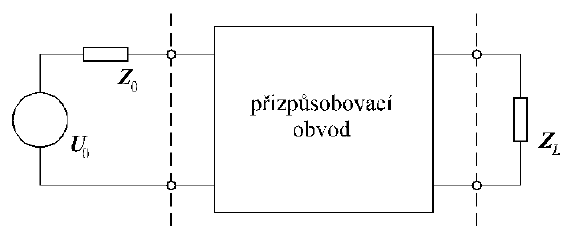
\includegraphics[width=0.5\linewidth]{RA_smith01.png}
          \caption{Umístění přizpůsobovacího obvodu mezi zátěží a zdrojem signálu (vedením)}
          \label{fyz:fig_RA_smith01} 
        \end{figure}
        K tomuto účelu vystačíme s nejjednodušším typem zapojení, které umožňuje dosažení 
        přizpůsobení na jednom kmitočtu s tzv. \(\Gamma\text{-články}\). Jde o kaskádní řazení 
        dvojice reaktančních prvků, z nichž jeden je vždy v podélné a druhý v příčné větvi bez 
        ohledu na pořadí. V rezistivních obvodech totiž dochází ke ztrátám přenášeného výkonu, 
        zatímco obvody složené z reaktancí slibují (alespoň teoreticky) dosažení přizpůsobení beze 
        ztrát. Kombinací obou pořadí s typy reaktančních prvků (kondenzátor, cívka) dostáváme 
        celkem osm různých možností uspořádání \(\Gamma\text{-článků}\), přičemž volba konkrétní 
        struktury závisí především na hodnotě přizpůsobované impedance \(Z_L\). Obrázek 
        \ref{RA:fig_smith02}  ukazuje jednotlivé vhodné struktury v závislosti na umístění 
        impedance \(Z_L\) v impedančním Smithově diagramu v jedné z osmi oblastí \emph{A} až 
        \emph{H}, při aplikaci požadavku přesunu z bodu \(Z_L\) do bodu \(Z_0\) co nejkratší 
        cestou. Hlavní myšlenka zde spočívá v tom, že do bodu \(Z_0\) se lze dostat jedině pohybem 
        po kružnici jednotkové reálné části impedance (\(r = 1\)) nebo admitance (\(y = 1\)), a to 
        buď po směru nebo proti směru hodinových ručiček. To zajišťuje první prvek 
        \(\Gamma\text{-článku}\) – sériově nebo paralelně řazený induktor nebo kapacitor. Z toho 
        plynou čtyři varianty označené malými písmeny „\emph{a}“ až „\emph{d}“. Úkolem 
        druhého stupně je přesun z bodu \(Z_L\) na jednu (obvykle tu nejbližší) z obou zmíněných 
        kružnic opět sériově nebo paralelně řazeným induktorem nebo kapacitorem – odtud tedy osm 
        variant přizpůsobení v oblastech \emph{A} až \emph{D}. Způsob návrhu 
        \(\Gamma\text{-článku}\) pomocí Smithova diagramu nejlépe objasníme na číselném příkladu.
  
        \begin{figure}[ht!] %\ref{RA:fig_smith02} 
          \centering
          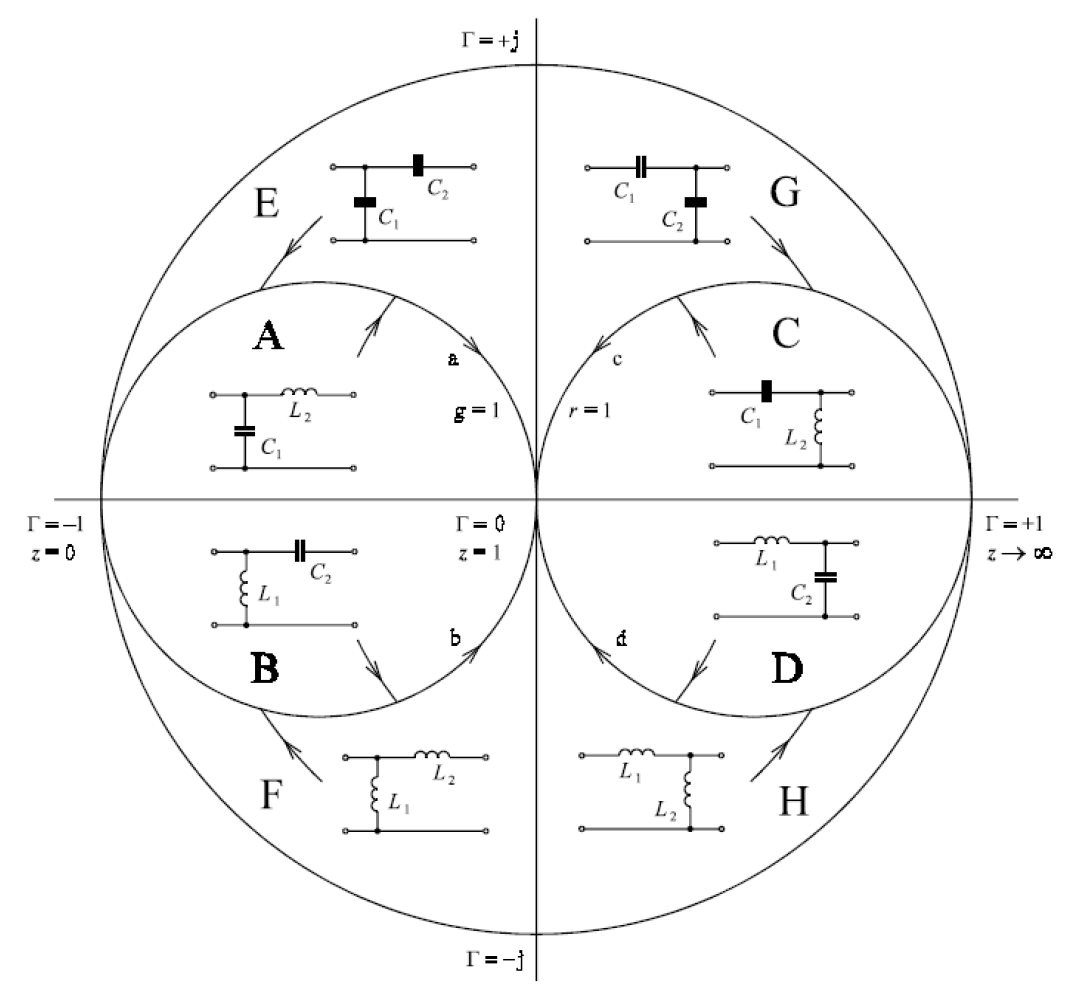
\includegraphics[width=\linewidth]{RA_smith02.png}
          \caption{Vhodné způsoby přesunu ve Smithově diagramu a odpovídající struktury  
          \(\Gamma\text{-článků}\)}
          \label{RA:fig_smith02} 
        \end{figure}
        %------------------------------------
          % !TeX spellcheck = cs_CZ
% RA_exam01.tex
\begin{example}
  Navrhněte graficko-početní metodou ve Smithově diagramu přizpůsobovací obvod pro 
  \(Z_L = \qty{30 - 65j}{\ohm}\) , \(Z_S = 50\)  a \(f = \qty{100}{\MHz}\).
  
  \textbf{Řešení:}
  Platí \(z_L = \dfrac{Z_L}{Z_S} = \num{0.6000 - 1.3000i}\), daný bod se tedy nachází ve 
  \textbf{4. kvadrantu}, \textbf{vně} kružnice konstantní reálné části impedance \(r = 
  1\). Proto volíme strukturu typu \(H\) viz. obr. \ref{RA:fig_smith02}. 
  \newline
  \begin{itemize}
    \item 1. krok: Začínáme v admitančních souřadnicích. Pro posun z bodu \(y_L = 
          \dfrac{1}{z_L} = \num{0.2927 + 0.6341i}\) nejkratší cestou na kružnici \(r = 1\), 
          tj. do bodu \(y_1 = \num{0.2927 + 0.4500i}\), musíme z admitance \(y_L\) ubrat 
          normovanou susceptanci \(\num{0.6341} - \num{0.4500} = \num{0.1841} = \Delta b = 
          \dfrac{\omega L_2}{Z_0}\). Paralelní indukčnost \(L_2\) tedy bude
          \MULTIPLY{2}{\numberPI}{\nmbrA}
          \MULTIPLY{\nmbrA}{100}{\nmbrB}
          \MULTIPLY{\nmbrB}{0.1841}{\nmbrC}
          \DIVIDE{50}{\nmbrC}{\nmbrD}
          \MULTIPLY{1000}{\nmbrD}{\nmbrE}
          \ROUND[2]{\nmbrE}{\sol}
          \begin{equation*}
            L_2 = \frac{Z_0}{\omega\abs{\Delta b}} = 
                  \frac{50}{2\cdot\pi\cdot\num{100e6}\cdot\num{0.1841}} = \qty{\sol}{\nano\henry}
          \end{equation*}
    
           {\centering   %\ref{RA:fig_RA_ADS_smith01} 
            \captionsetup{type=figure}
            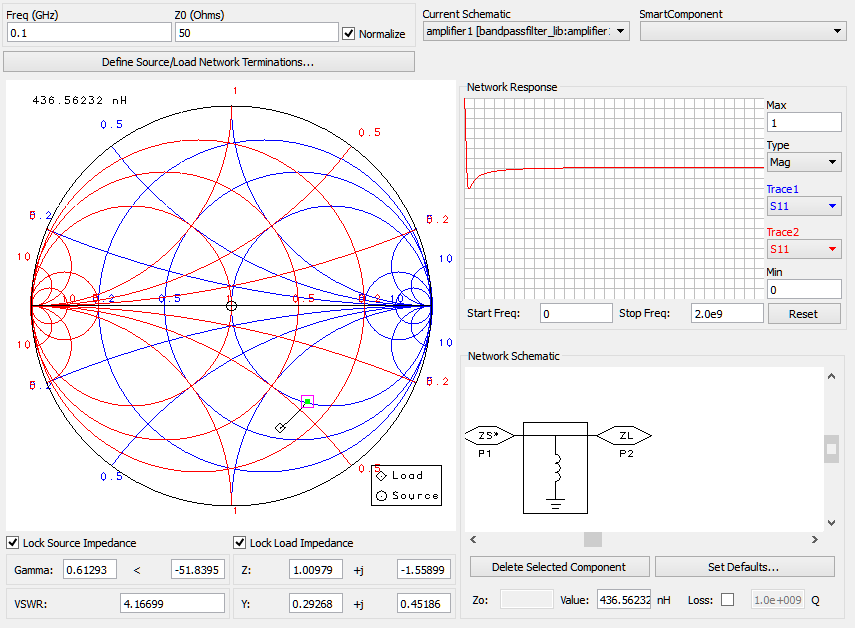
\includegraphics[width=0.8\linewidth]{ADS_smith01.png}
            \captionof{figure}{ADS Smith Chart tool: Přechod z bodu \(y_L \rightarrow y_1\)}
            \label{RA:fig_ADS_smith01} 
            \par}
          
    \item 2.krok: Pro posun z bodu \(z_1 = \dfrac{1}{y_1} = \num{1 - 1.5479i}\) do bodu 
          \(z_S = \num{1 + 0i}\) musíme k \(z_1\) přidat normovanou reaktanci \(1.5479 = \Delta 
          x = \frac{\omega L_2}{Z_0}\). Sériová indukčnost \(L_1\) tedy bude
          \MULTIPLY{2}{\numberPI}{\nmbrA}
          \MULTIPLY{\nmbrA}{100}{\nmbrB}
          \MULTIPLY{50}{1.5479}{\nmbrC}
          \DIVIDE{\nmbrC}{\nmbrB}{\nmbrD}
          \MULTIPLY{1000}{\nmbrD}{\nmbrE}
          \ROUND[2]{\nmbrE}{\sol}
          \begin{equation*}
            L_1 = \frac{\Delta x Z_0}{\omega} = 
                  \frac{\num{1.5479}\cdot\num{50}}{2\cdot\pi\cdot\num{100e6}} = 
                  \qty{\sol}{\nano\henry}
          \end{equation*}
           
           {\centering   %\ref{RA:fig_RA_ADS_smith02}
            \captionsetup{type=figure} 
            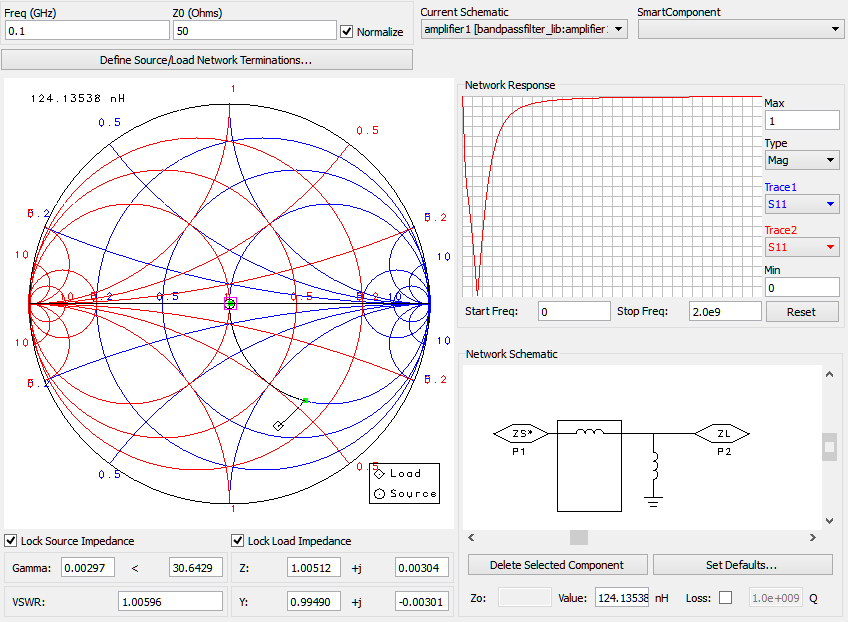
\includegraphics[width=0.8\linewidth]{ADS_smith02.png}
            \captionof{figure}{ADS Smith Chart tool: Přechod z bodu \(z_1 \rightarrow z_S\)}
            \label{RA:fig_ADS_smith02} 
            \par} 
  \end{itemize}
\end{example} 
        %------------------------------------
        Kromě přesunu nejkratší cestou přicházejí v úvahu ještě další varianty spojené s přechodem 
        do jiného segmentu. Např. pro \(Z_L\) v oblasti \(A\) lze použít též 
        \(\Gamma\text{-článek}\) typu \(B\); pro \(Z_L\) v oblasti \(E\) lze použít též typy \(B\), 
        \(D\) nebo \(G\) apod. Pro dosažení nejmenší kmitočtové závislosti lze však obvykle 
        doporučit pouze přesun nejkratší cestou.
  
      \subsubsection{Smithův diagram}
        \emph{Impedanční Smithův diagram} je soustava křivek (přesněji kružnic nebo jejich částí) 
        tvořených body normované impedance \(z\) s konstantní reálnou či imaginární částí 
        zakreslených v komplexní rovině činitele odrazu \(\Gamma\) definovaná konformním zobrazením
        \begin{equation}\label{RA:eq_smith07}
          \Gamma = \frac{z-1}{z+1}.
        \end{equation} 
  
        Každému bodu v Smithově diagramu odpovídá jedna hodnota normované impedance \(z = r + jx\), 
        a odnormované impedance \(Z = R+jX\). Otočením o 180°, popř. středovou souměrností, 
        získáme \emph{admitanční Smithův diagram} \(y = g + jb\), resp. \(Y = G + jB\). Kružnice 
        konstantních reálných částí se sbíhají v bodě \(1\) a mají středy na reálné ose. Kružnice 
        (části kružnic) konstantní imaginární části se taktéž sbíhají v bodě \(1\) a mají středy na 
        přímce Re [] = 1.
  
        Jelikož pro převod mezi poměrem stojatých vln a modulem činitele odrazu j􀀀j platí stejný 
        vztah jako mezi činitelem odrazu 􀀀 a normovanou impednací z, tj.
        \begin{equation}\label{RA:eq_smith08}
          \Gamma = \frac{z-1}{z+1} \qquad \Leftrightarrow 
          \abs{\Gamma} = \frac{\abs{PSV}-1}{z+\abs{PSV}}.
        \end{equation} 
        s rozdílem, že PSV je vždy reálné číslo větší nebo rovno jedné, lze PSV pro daný bod ve 
        Smithově diagramu určit z průsečíku kružnice se středem v bodě z = 0 a poloměrem j􀀀j a 
        části reálné osy normované impedance mezi body z = 1 a z ! 1.
        
      \subsubsection{Měření činitěle odrazu} 
        Abychom mohli měřit činitel odrazu podle definice (1), musíme mít možnost
        \begin{itemize}
          \item oddělit vlnu odraženou (U¡) od vlny dopadající (U+)
          \item měřit komplexní poměr fázorů napětí na příslušném kmitočtu.
        \end{itemize} 
        
        Splnění prvního požadavku nám zajišťuje tzv. směrový vazební člen (SVČ), splnění druhého 
        požadavku pak vektorový voltmetr. Celkové uspořádání měřicí sestavy využívající směrového 
        vazebního členu a vektorového voltmetru znázorňuje obr. 3. Harmonický signál potřebného 
        kmitočtu se rozděluje pomocí symetrického přizpůsobeného T-článku (splitteru) do tzv. 
        referenční a měřicí větve. Obě větve jsou zakončeny terminátory o impedanci rovné vlnové 
        impedanci Z0 vedení a konektorů, aby zde nedocházelo k nežádoucím odrazům a stojatému 
        vlnění. Ke snížení stojatého vlnění též přispívají pevné útlumové články v obou větvích 
        (20, 14 a 6 dB). Napětí v obou větvích jsou snímána sondami vektorového voltmetru 
        zasunutými do průchozích držáků. Měřená zátěž ZL je připojena na konec hlavního vedení 
        směrového vazebního členu SVč . Odražená vlna se potom vyvazuje na bránu 4 (přes vazbu K2 
        SVČ) a její amplituda a fáze je měřena sondou B vektorového voltmetru. Sonda A v referenční 
        větvi poskytuje fázovou referenci pro stanovení fáze činitele odrazu.
  
        Měření činitele odrazu probíhá ve dvou krocích:
        \begin{itemize}
          \item Nastavení amplitudové a fázové referenční hodnoty. Měřicí aparaturu je třeba 
          zkalibrovat tak, aby udávaný modul a fáze činitele odrazu pro nějakou zátěž, jejíž 
          činitel odrazu předem známe, této hodnotě přesně odpovídal. K tomuto účelu se obvykle 
          používá zkrat (Z = 0, 􀀀 = ¡1;0), ale v našem konkrétním případě se jako vhodnější ukazuje 
          otevřený konec vedení (Z ! 1, 􀀀 = +1;0), neboť naměřená odražená vlna při něm vykazuje o 
          něco větší amplitudu než při zakončení zkratem. Bránu 3 SVč (konec hlavního vedení) tedy 
          necháme nezakončenou a na generátoru nastavíme příslušný kmitočet f a vhodnou amplitudu 
          (zpravidla největší přípustnou, pro dobrý odstup signálu od šumu ve vektorovém 
          voltmetru). Amplitudu napětí naměřenou v této situaci sondou B uložíme na přístroji 
          BM553 jako referenční stlačením tlačítek <B>, <LEVEL REF STORE> a fázový rozdíl 'B ¡'A 
          uložíme jako referenční tlačítkem <',T REF STORE>. Aplikaci uložené amplitudové 
          referenční hodnoty poté aktivujeme tlačítkem <LIN REF>. Přístroj by měl zobrazovat 
          správnou hodnotu 􀀀 pro zakončení naprázdno, tj. modul 1;0 a fázi 0±.
  
          \item Vlastní měření činitele odrazu 􀀀. Na bránu 3 směrového vazebního členu připojíme 
          měřenou zátěž. Bylo-li provedeno nastavení podle předchozího bodu, bude již přístroj 
          ukazovat správnou hodnotu činitele odrazu 􀀀 v polárních souřadnicích.   
        \end{itemize}
        
        Z uspořádání měřicího systému je zřejmé, že při měření činitele odrazu na více kmitočtech 
        je třeba po každé změně kmitočtu signálu celý první krok postupu zopakovat.
  
      \subsubsection{Směrový vazební člen}     
        Směrový vazební člen (SVČ, též směrová vazební odbočka, směrová vazební odbočnice, směrová 
        vazba) je vysokofrekvenční čtyřbran umožňující oddělení a měření složek signálu, které se 
        šíří po vedení pouze jedním směrem. Mezi jeho četné aplikace patří měření činitele odrazu, 
        oddělení signálního generátoru od měřicích obvodů, rozdělení výkonu a připojení dalších 
        přístrojů (vlnoměrů, analyzátorů, wattmetrů apod.).
  
        Princip SVČ je založen na vlastnostech obvodů s rozprostřenými parametry a jeho vnější 
        funkce je patrná z obrázku 4. Dva úseky vedení ‚- hlavní (zakončené branami 1 a 3) a 
        vedlejší/vazební (mezi branami 2 a 4) ‚- jsou spojeny tak, aby mezi nimi vznikla vazba. 
        Tato vazba způsobuje, že se signál zavedený na bránu 1 hlavního vedení rozdělí v určitém 
        poměru na dvě vzájemně fázově posunuté složky. Jedna složka vystupuje na bráně 3 a druhá 
        bud’ na bráně 2, přičemž brána 4 je dokonale izolována (protisměrný SVČ ), nebo na bráně 4, 
        přičemž brána 2 je izolována (souměrný SVČ ). Zmíněná vazba je reciprocitní a vykazuje 
        obdobné chování i ze směru od vedlejšího vedení k hlavnímu.      
  
        \begin{figure}\ref{fyz:fig_RA_smith03} 
          \centering
          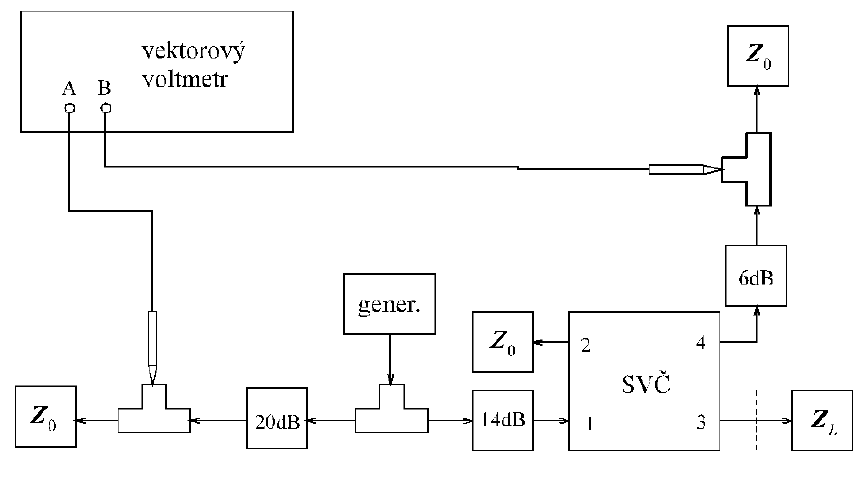
\includegraphics[width=\linewidth]{RA_smith03.png}
          \caption{Směrový vazební člen jako čtyřbran}
          \label{fyz:fig_RA_smith03} 
        \end{figure}
  
        SVČ lze popsat maticí rozptylových parametrů o rozměru 4 Q 4, kde parametry skk na hlavní 
        diagonále jsou činitele odrazu na jednotlivých branách, ostatní parametry jsou činitele 
        přenosu mezi branami. U ideálního protisměrného (obr. 4) SVč jsou všechny činitele odrazu 
        rovny nule, přenos z brány 1 na bránu 4 je též nulový a s ohledem na symetrii SVč jsou 
        nulové i přenosy mezi branami 4–1, 2–3 a 3–2. Rozptylová matice ideálního SVč potom tedy je
  
        \begin{equation}\label{RA:eq_smith09}
          s = \left[
            \begin{matrix}
                0    & s_{12} & s_{13} &  0       \\
              s_{21} &   0    &   0    & s_{24}   \\
              s_{31} &   0    &   0    & s_{34}   \\
                0    & s_{42} & s_{43} &  0     
            \end{matrix}
              \right]
        \end{equation} 
  
        Vzhledem k aplikaci SVč a symetrii matice s-parametrů se SVč často charakterizují několika 
        skalárními parametry vycházejícími z s-parametrů resp. výkonové bilance na branách SVč . 
        Jsou to tyto parametry: vazba K (K1, K2, též tzv. přeslechový útlum), směrovost D, izolace 
        I a taktéž kmitočtový rozsah.
  
        Vazba K (též K1) je definována jako poměr výkonu P1 přiváděného na vstup hlavního vedení 1 
        a výkonu P2 vystupujícího z brány 2 při bezodrazovém zakončení bran 2 až 4,
        \begin{equation}\label{RA:eq_smith10}
          K = K_1 = 10\log\frac{P_1}{P_2} 
                  = 10\log\frac{1}{\abs{s_{21}}^2} = -20\log\abs{s_{21}},  
        \end{equation} 
        a vyjadřuje tedy vazební útlum přímé vlny na hlavním vedení (směřující od brány 1 k bráně 
        3) na vstup vedlejšího vedení 2.
  
        Podobně vazba K2 je definována jako poměr výkonu P3 přiváděného na výstup hlavního vedení 3 
        a výkonu P4 vystupujícího z brány 4 při bezodrazovém zakončení bran 1, 2 a 4,
        \begin{equation}\label{RA:eq_smith11}
          K_2 = 10\log\frac{P_3}{P_4} 
              = 10\log\frac{1}{\abs{s_{43}}^2} = -20\log\abs{s_{43}},  
        \end{equation} 
        a vyjadřuje tedy vazební útlum zpětné vlny na hlavním vedení (směřující od brány 3 k bráně 
        1) na výstup vedlejšího vedení 4.
  
        Směrovost D je definována jako poměr výkonu P2 vystupujícího z brány 2 a výkonu P4 
        vystupujícího z brány 4 při přivádění signálu na bránu 1 a bezodrazovém zakončení bran 2 až 
        4,
        \begin{equation}\label{RA:eq_smith12}
          D = 10\log\frac{P_2}{P_4} 
            = 10\log\frac{1}{\abs{s_{42}}^2} = -20\log\abs{s_{42}},  
        \end{equation} 
  
        Izolace I je definována jako poměr výkonu P1 přiváděného na vstup hlavního vedení 1 a 
        výkonu P4 vystupujícího z brány 4 při bezodrazovém zakončení bran 2 až 4,
        \begin{equation}\label{RA:eq_smith13}
          I = 10\log\frac{P_1}{P_4} 
            = 10\log\frac{1}{\abs{s_{41}}^2} = -20\log\abs{s_{41}}, 
        \end{equation} 
        a vyjadřuje tedy vazební přeslechový útlum mezi přímou vlnou na hlavním vedení (směřující 
        od brány 1 k bráně 3) a výstupem vedlejšího vedení 4.
  
        Z uvedených definic plyne, že směrovost D je rovna rozdílu izolace I a vazby K (resp. K1)
        \begin{equation}\label{RA:eq_smith14}
          D = I - K = I - K_1 = 20\log\frac{\abs{s_{21}}}{\abs{s_{41}}}
        \end{equation}  
  
        Směrovost D (v souladu se svým názvem) popisuje schopnost směrové selekce – čím je větší, 
        tím méně se při měření vlny signálu v jednom směru pomocí SVč nežádoucím způsobem projevuje 
        vlna šířící se v opačném směru.
  
      \subsection{Vektorový voltmetr}
        Vektorový voltmetr je schopen měřit amplitudy dvou harmonických signálů \(U_A\) a \(U_B\) a 
        jejich fázový rozdíl \(\varphi_B - \varphi_A\). Dále bývá obvykle schopen měřit poměr 
        amplitud \(\frac{U_B}{U_A}\) a také umožňuje i relativní měření vůči uložené a různá 
        odvozená měření (např. s-parametrů, R, L, C prvků apod.) využívající zvláštní příslušenství.
  
        Princip vektorového voltmetru je založen na vzorkování obou měřených signálů a jejich 
        současném převodu na nízký mezifrekvenční kmitočet 20 kHz. Takto nízký kmitočet lze již 
        snadno a přesně zpracovat, jednak detektory a A/D převodníky pro zjištění amplitudy, jednak 
        logickými obvody pro zjištění fázového rozdílu. Vzorkování se provádí velmi rychlými 
        analogovými spínači se Schottkyho diodami umístěnými přímo v sondách. Vzorkovací kmitočet 
        se musí od kmitočtu měřeného signálu lišit přesně o 20 kHz, což je zajištěno pomocí smyčky 
        automatické kmitočtové a fázové synchronizace uvnitř voltmetru.  

%---------------------------------------------------------------------------------------------------
\printbibliography[heading=subbibliography]
\addcontentsline{toc}{section}{Seznam literatury}
  % %============= Kapitola: Simthův diagram v radiotechnice  ==========================================
\setchaptertoc
\chapter{Simthův diagram v radiotechnice}\label{chap:ra_smith}


    \begin{figure}[ht!]  % \ref{fig_RA:modulace04}
      \centering
      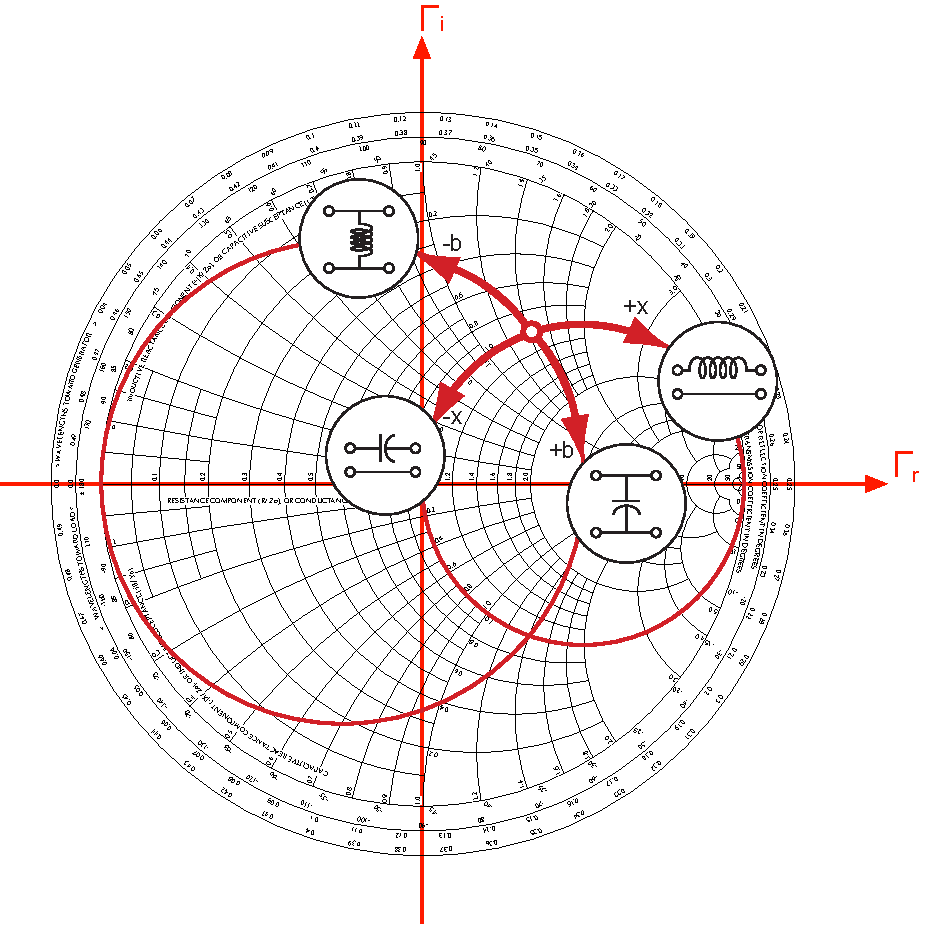
\includegraphics[width=1\linewidth]{smith_chart01.pdf}
      \caption{Smith Chart: Effect of Adding Series Reactances or Shunt Susceptances 
               \cite[s.~45]{IEEEStearns2001}}
      \label{fig_RA:smith01}
    \end{figure}
    
%---------------------------------------------------------------------------------------------------
  % % !TeX spellcheck = cs_CZ
%=============== Kapitola: Antény: Teoretický základ ===============================================
\chapter{Antény: Teoretický základ}\label{chap:ra_antennatheory}
\minitoc

  \section{Teoretický základ}
    Když jsme se na počátku našeho výkladu zabývali šířením vln, nezajímali jsme se o to, jak vlny 
    vznikly. Proces vzniku vlnění v prostoru (proces vyzařování) bude vyšetřováno v této kapitole. 
    
    Z fyziky je známo, že zdrojem elektromagnetických vln je střídavý (vysokofrekvenční) proud. 
    Úlohu o vyzařování můžeme tedy formulovat tak, že známe proud tekoucí v prostoru (na vysílací 
    anténě) a chceme zjistit, jaké intenzity polí vytvoří tento proud kdekoli jinde v prostoru. 
    Matematicky jde o \textbf{řešení nehomogenní soustavy Maxwellových rovnic:}
    \begin{align}\label{RA:eq_ant01}
      \rot{H} &= \vec{J} + j\omega\varepsilon\vec{H} \\
      \rot{E} &= -j\omega\mu\vec{H}
    \end{align}
    v níž proudová hustota \(\vec{J}\) je známá a intenzity \(\vec{E}\) a \(\vec{H}\) se hledají 
    \cite[s.~33]{Hanus2002}. 
    
    \subsection{Impedance lineárních antén}
      Lineární anténa je \emph{jednobran} a poměr fázorů vstupního napětí a vstupního proudu 
      definuje  tzv. \textbf{vstupní impedanci antény}. Vstupní impedance je veličina stejně 
      důležitá jako funkce záření, protože rozhoduje o přizpůsobení antény k napájecímu vedení. 
      Vstupní impedance je obecně komplexní: má reálnou část (\emph{vstupní odpor}) a imaginární 
      část (\emph{vstupní reaktanci}). Obě složky bezprostředně souvisí s činností antény. Anténa 
      vyzařuje jistý činný výkon, a tudíž nejméně stejný činný výkon musí také odebírat ze zdroje. 
      Z hlediska uživatele se musí jevit na svorkách antény takový reálný odpor, který by odebíral 
      tentýž výkon. Ve skutečnosti má anténa ztráty (část přivedeného činného výkonu se mění v 
      teplo), takže odebíraný výkon bude o něco větší a odpor na svorkách také. Kromě toho anténa 
      během každé periody si vyměňuje energii s elektromagnetickým polem ve svém blízkém 
      okolí a to se projeví existencí jisté reaktance na vstupu. Této úvaze odpovídá náhradní obvod 
      antény nakreslený na obr. \ref{RA:fig_001} \cite[s.~44]{Hanus2002}.

      \begin{figure}[ht!]   %\ref{RA:fig_001}
        \centering
        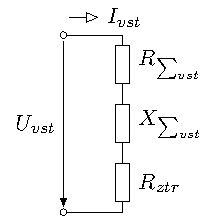
\includegraphics[width=0.5\linewidth]{RA001.pdf}
        \caption{Náhradní obvod antény}
        \label{RA:fig_001}
      \end{figure}
      
      Odpor \(R_{\sum_{vst}}\) je tzv. \textbf{odpor záření antény} vztažený ke vstupnímu proudu. 
      Místo odpor záření se užívají také názvy \emph{vyzařovací odpor} nebo \emph{zářivý odpor}. 
      Odpor  \(R_{ztr}\) je \textbf{ztrátový odpor antény}. V součinu se čtvercem efektivní hodnoty 
      vstupního proudu tyto odpory určují \textbf{vyzařovaný a ztrátový výkon antény}:
      \begin{itemize}\addtolength{\itemsep}{-0.5\baselineskip}
        \item \emph{vyzařovaný výkon:} \(P_{\sum} = I^2_{vst_{ef}}\cdot R_{\sum_{vst}}\)
        \item \emph{ztrátový výkon:}   \(P_{ztr} = I^2_{ztr_{ef}}\cdot R_{ztr}\)
      \end{itemize}
      Protože na anténě je obvykle stojaté vlnění, je proud v každém místě jiný. Vyzařovaný výkon 
      je však jeden. Podle prvního z uvedených vztahů přísluší tedy každému proudu, a tedy i 
      každému místu na anténě, jiná hodnota odporu záření. Nebo naopak, každá hodnota odporu záření 
      je \emph{vztažena} k určitému proudu (místu) na anténě. Nejčastěji se odpor záření vztahuje 
      buď k proudu vstupnímu (\(I_{vst}\)) nebo k proudu v kmitně (\(I_{max}\)). Vyzařovaný výkon 
      je tedy alternativně
      \begin{equation}\label{RA:eq_ant02}
        P_{\sum} = I^2_{vst_{ef}}\cdot R_{\sum_{vst}} = I^2_{max_{ef}}\cdot R_{\sum_{m}}
      \end{equation} 
      \(R_{\sum_{m}}\) je \emph{odpor záření vztažený ke kmitně proudu}. Vztah (\ref{RA:eq_ant02}) 
      umožňuje přepočítat odpor záření z jednoho místa do druhého, známe-li funkci \emph{proudové 
      distribuce}. 
      
      
     
  \section{Parametry antén}
    Elektrické vlastnosti antén různých typů se charakterizují stručnými číselnými údaji, které 
    nazýváme parametry. Jejich znalost je důležitá při navrhování rádiových soustav 
    \cite[s.~46]{Hanus2002}. 

     % In many situations, a good match is defined arbitrarily as having SWR<1.5. 
     V mnoha aplikacích se dosažené impedanční přizpůsobení považuje dobré je-li \(\text{VSWR}<1,5\)
     \begin{align}
       \text{VSWR} &= \frac{1+\abs{\Gamma}}{1-\abs{\Gamma}} \qquad \Rightarrow \qquad
                     \abs{\Gamma} = \frac{\text{VSWR}-1}{\text{SWR}+1}, \\
       \shortintertext{a odražený výkon lze jednoduše získat jako mocninu amplitudy koeficientu 
         odrazu} 
       R_L &= -10\log\abs{\Gamma}^2 = -20\log\abs{\Gamma} \qquad\si{\decibel} \\
       \shortintertext{and the transmitted power to the load, relative to the incident wave power, 
         is}
       T_L &= -10\log(1 - \abs{\Gamma}^2) \qquad\si{\decibel}
     \end{align}
     
     
    \begin{table}[ht!]
      \centering
      \begin{tabular}{c|ccc}
        \rowcolor[HTML]{000000} 
        \multicolumn{1}{c}{\cellcolor[HTML]{000000}
          {\color[HTML]{FFFFFF} \textbf{VSWR}}}      & 
          {\color[HTML]{FFFFFF} \textbf{\(\abs{\Gamma}\)}} & 
        \multicolumn{2}{c}{\cellcolor[HTML]{000000}
          {\color[HTML]{FFFFFF} \textbf{Odražený výkon}}}          \\ 
        \rowcolor[HTML]{000000}{\color[HTML]{FFFFFF} }           &
                               {\color[HTML]{FFFFFF} \(\abs{s_{11}}\)}  & 
                               {\color[HTML]{FFFFFF} (\%)}       & 
                               {\color[HTML]{FFFFFF} (dB)}           \\
         1.0 & 0.000 &  0.0 & \(\infty\)  \\
         1.5 & 0.200 &  4.0 & 14.0  \\
         2.0 & 0.333 & 11.1 & 9.55  \\
         2.5 & 0.429 & 18.4 & 7.36  \\
         3.0 & 0.500 & 25.0 & 6.00  \\
         3.5 & 0.556 & 30.9 & 5.10  \\
         4.0 & 0.600 & 36.0 & 4.44  \\
         5.0 & 0.667 & 44.0 & 3.52  \\
         6.0 & 0.714 & 51.0 & 2.92  \\
         7.0 & 0.750 & 56.3 & 2.50  \\
         8.0 & 0.778 & 60.5 & 2.18  \\
         9.0 & 0.800 & 64.0 & 1.94  \\
        10.0 & 0.818 & 66.9 & 1.74  \\
        15.0 & 0.875 & 76.6 & 1.16  \\
        20.0 & 0.905 & 81.9 & 0.87  \\
        50.0 & 0.961 & 92.3 & 0.35  \\ \cline{1-4}
        \hline
      \end{tabular}
      \caption{Demonstrace vzájemného vztahu mezi poměrem stojatých vln \texttt{VSWR}, amplitudy 
               koeficientu odrazu \(\Gamma\) a velikostí odraženého výkonu\protect\footnotemark[1] 
               vyjádřeného v procentech a decibelech. Kredit: \AntTheoVSWR}
      \label{fig_RA:VSWRGammaTable}
    \end{table}

 \footnotetext[1]{Return loss}

%---------------------------------------------------------------------------------------------------
\printbibliography[heading=subbibliography]
\addcontentsline{toc}{section}{Seznam literatury}
  % % !TeX spellcheck = cs_CZ
%============= Kapitola: Modulace===================================================================
\setchaptertoc
\chapter{Modulace}\label{chap:ra_mod}


  %--------------- Rádiové komunikační systémy ----------------==-----------------------------------
  \section{Obecné schéma rádiového komunikačního systému}
    V této kapitole jsou shrnuty základní poznatky o modulacích používaných v rádiové komunikaci. 
    Nejprve se popišme obecné schéma rádiového komunikačního systému podle Shannona, které je na 
    obr. \ref{fig_RA:modulace01}. Toto schéma lze aplikovat především na systémy digitální, tedy 
    například na systémy digitálního rozhlasu a televize, na systémy digitálních celulárních 
    radiotelefonů, na systémy digitálních radiokomunikačních družicových prostředků apod. 
    \begin{figure}[ht!]  % \ref{fig_RA:modulace01}
      \centering
      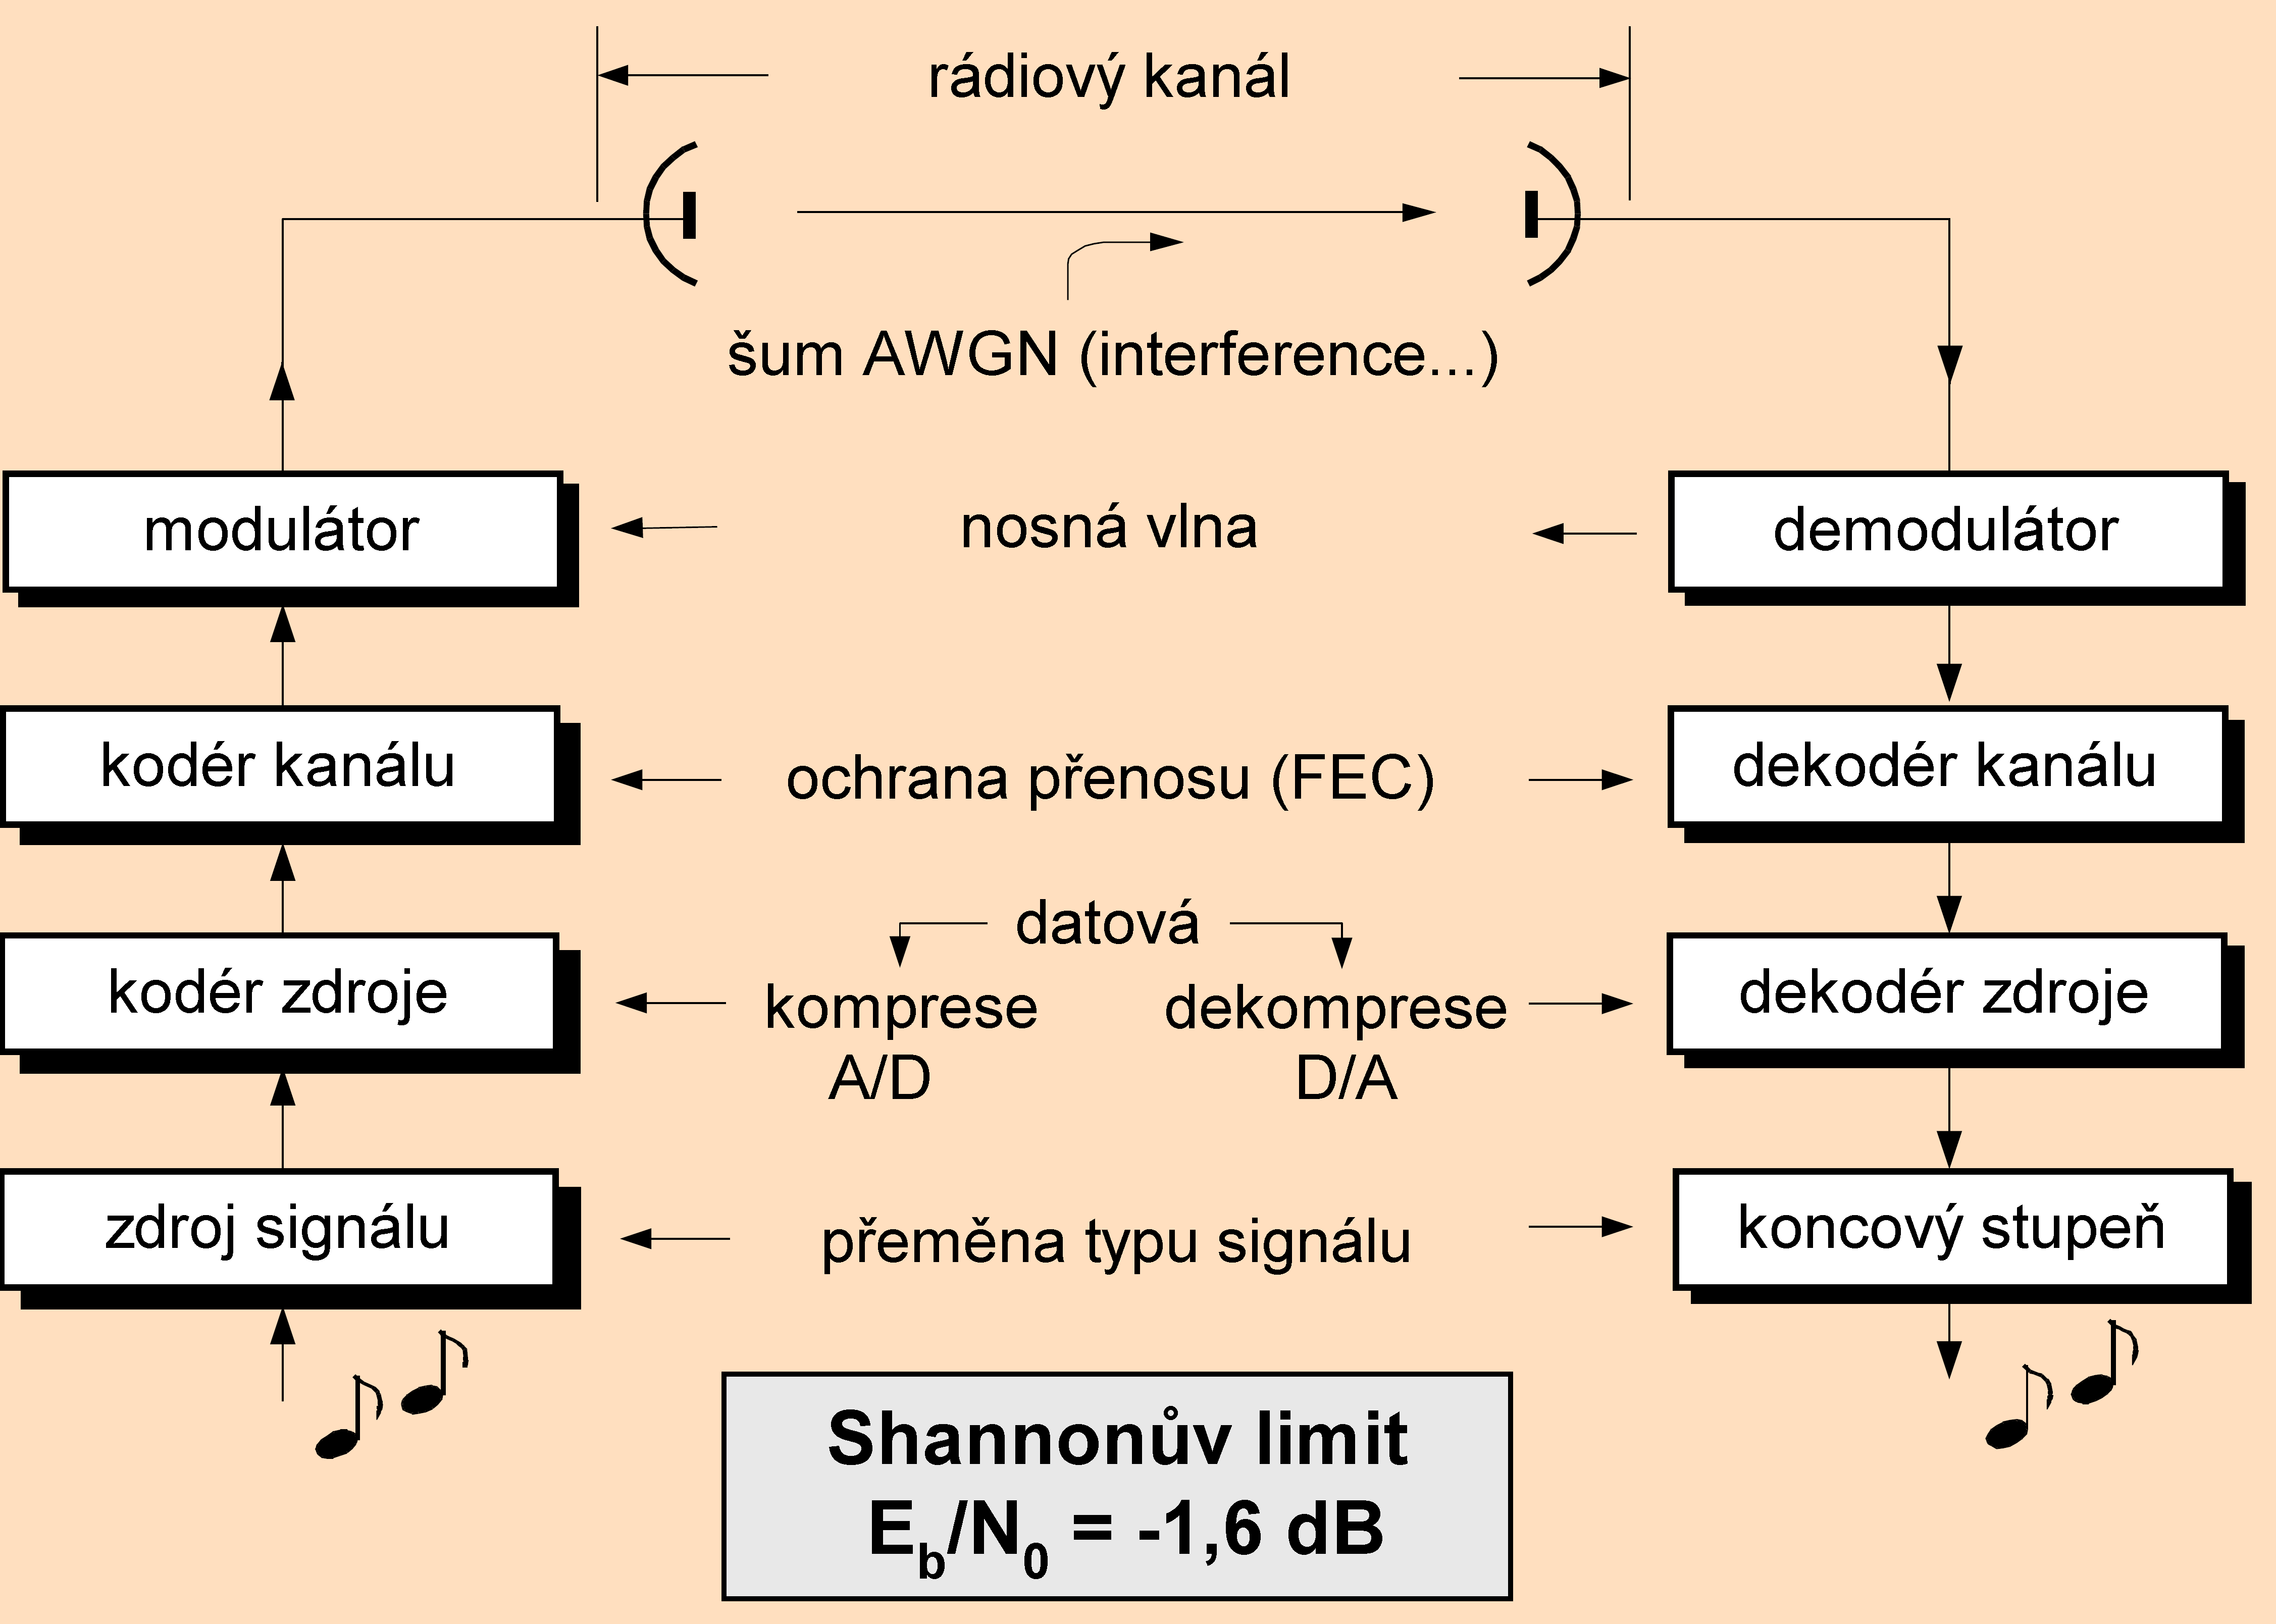
\includegraphics[width=1\linewidth]{shannon_radiokomunikacni_system.png}
      \caption{Obecné Shannonovo schéma radiokomunikačního systému
               \cite[s.~75]{ZaludRA}}
      \label{fig_RA:modulace01}
    \end{figure}
    
    Pokud se však v tomto schématu vypustí některé bloky (kodéry a dekodéry), je použitelné i pro 
    vývojově starší analogové systémy. Přestože toto schéma koncipoval Shannon již v padesátých 
    letech, je dodnes aktuální a po menších úpravách lze pomocí něho modelovat i nejmodernější 
    radiokomunikační zařízení.
    
    Na vstupu vysílače je \textbf{zdroj signálu}, jímž může být např. mikrofon nebo televizní 
    snímací elektronka apod. Ten pře\-mě\-ňu\-je přenášenou informaci, jež může mít v obecném 
    případě původně charakter neelektrické veličiny, na elektrický signál. V následujícím 
    \textbf{kodéru zdroje signálu} se signály přicházející z předchozího bloku nejprve digitalizují 
    (pokud ovšem neměly již předtím digitální podobu) a poté se podrobují vlastnímu zdrojovému 
    kódování. Tím se v nich potlačuje \emph{redundance}, což je nadbytečná informace, která je v 
    akustických, obrazových či jiných informačních tocích pocházejících z „přírodních“ zdrojů 
    většinou velmi výrazně zastoupena; (přesněji bývá redundance definována jako nadbytečnost, 
    resp. větší množství dat, než je nezbytné pro přenos informace vzhledem ke ztrátám v 
    komunikačním kanálu; dokonalá exaktní definice této veličiny je však složitá). Zde se potlačuje 
    také irelevance, volně definovaná jako nepodstatná informace. Účinnost kódování prováděného v 
    kodéru zdroje je tím lepší, čím je rychlost bitového toku na jeho výstupu nižší, než na jeho 
    vstupu; připomeňme, že proces zdrojového kódování se proto také označuje jako proces 
    \emph{komprese dat}, nebo také jako mapování vstupního digitálního signálu zdrojového kodéru na 
    jeho signál výstupní. Toto mapování se uskutečňuje podle určitého jednoznačného algoritmu. 
    Dekodér zdroje signálu na přijímací straně realizující inverzní mapování, již poskytuje na svém 
    výstupu užitečný výstupní signál, který se většinou až na zkreslení, šum a určitou složku 
    neobnovené redundance shoduje se signálem na vstupu kodéru zdroje.
        
    V následujícím \textbf{kodéru kanálu} se k binární užitečné - redundance a irelevance, alespoň 
    částečně zbavené - informační sekvenci naopak určitá \emph{redundantní} složka přidává. Je to 
    však redundance přesně kontrolovaná, která je potom využívána k potlačení rušivého působení 
    šumu a interferencí, způsobujících chybovost přenosu. V nejjednodušších (triviálních) systémech 
    kanálového kódování se prostě každý informační bit přenáší m-krát, kde \(m\) je celé kladné 
    číslo. U složitějších (netriviálních) systémů se informační tok sdružuje do sekvencí po \(k\) 
    bitech, k nimž se potom podle vhodných algoritmů přiřazují („mapují“) určité zakódované 
    sekvence po \(n\) bitech. Objem redundance, která se tímto způsobem přidává k užitečnému 
    signálu, je dán poměrem \(n/k\); reciproká hodnota tohoto poměru \(R_c = k/n\) se potom 
    označuje \emph{rychlost kanálového kódování}, nebo krátce \emph{rychlost}. \emph{Zvýšení 
    rychlosti bitového toku signálu způsobené kanálovým kódováním si bohužel vynucuje i rozšíření 
    potřebné šířky pásma komunikačního kanálu mezi vysílačem a přijímačem}.
    
    Uvedeným dvojím kódováním se získává digitální signál s potlačenou redundancí a irelevancí a se 
    zvýšenou odolností proti faktorům způsobujícím chybovost. Ten dále vchází do 
    \textbf{modulátoru}, kde se moduluje pomocí vhodného digitálního modulačního způsobu (formátu) 
    na vysokofrekvenční, nebo na mikrovlnnou nosnou vlnu. \emph{Modulace} je obecně definována jako 
    \emph{proces, při němž se některý parametr této nosné vlny (amplituda, kmitočet, fáze) mění v 
    rytmu modulačního signálu (definice podle Standardu IEEE)}. Díky využití principů modulace je 
    potom možné přenášet v určitém rádiovém prostředí, na nosných vlnách s různými kmitočty, velké 
    množ\-ství zcela nezávislých modulačních signálů. Některé typy modulací navíc umožňují v 
    procesu demodulace v přijímači zlepšit odstup užitečného signálu od šumu, i když za cenu 
    vyšších nároků na šířku pásma. Kromě toho lze při použití nosných vln o relativně vysokých 
    kmitočtech snáze realizovat vysílací i přijímací antény, účinně převádějící elektrický výstupní 
    výkon vysílačů na elektromagnetické vlny, šířící se potom rádiovým komunikačním kanálem. Zcela 
    obecně lze tedy definovat optimální modulátor jako funkční blok, který co nejlépe přizpůsobuje 
    přenášený modulační signál k parametrům následujícího rádiového komunikačního kanálu. Optimální 
    demodulátor potom naopak přijímaný signál převádí - opět pokud možno co nejvěrněji - na původní 
    modulační signál.
    
    \textbf{Komunikačním kanálem} se obecně rozumí fyzikální pros\-tře\-dí, sloužící k přenosu 
    signálu mezi vysílačem a přijímačem. V případě rádiového kanálu toto pojetí odpovídá schématu 
    na obr. \ref{fig_RA:modulace01}, někdy se však do „kanálu“ zahrnují ještě i výstupní obvody 
    vysílačů a vstupní obvody přijímačů apod., takže v zájmu jednoznačnosti je nezbytné tento 
    termín vždy přesně specifikovat. Kromě zmíněných rádiových kanálů se v praxi uplatňují také 
    vývojově vůbec nejstarší kanály s metalickými spoji používané původně v telegrafii a v 
    telefonii, v novější době potom i kanály s optickými spoji.
    
    \emph{Rádiový komunikační kanál} je specifikován určitými parametry, které mohou mít jednak 
    náhodný a jednak nenáhodný charakter. K užitečnému přenášenému signálu se zde především přidává 
    náhodný šum, o němž se v teoretických úvahách v prvém přiblížení předpokládá, že je to 
    \emph{aditivní bílý Gaussov\-ský šum \texttt{AWGN} (Additive White Gaussian Noise)} připomeňme, 
    že pojem \emph{aditivní} zde značí šum, který se lineárně sčítá s užitečným signálem, aniž by 
    docházelo ke vzájemným intermodulacím; pojem \emph{bílý} označuje šum, jehož výkonová 
    spektrální hustota je konstantní tj. nezávislá na kmitočtu a termín \emph{Gaussovský} potom 
    vyjadřuje skutečnost, že rozložení okamžitých amplitud tohoto šumu se řídí \emph{Gaussovou 
    distribucí}. Do komunikačního kanálu přicházejí dále nejrůznější náhodná \emph{rušení} tj. 
    \emph{interference}, ať již přírodního původu (atmosférické poruchy apod.), nebo pocházející od 
    „průmyslových“ zdrojů (od zapalovacích systémů automobilů, atd.). Mohou se zde však uplatňovat 
    ještě další náhodné jevy jako jsou různé typy \emph{úniků (fadingu)} apod. Kromě těchto 
    parametrů náhodného charakteru zde může být přenos signálu ovlivňován ještě dalšími efekty, 
    které mohou mít za určitých okolností nenáhodný tj. deterministický charakter. Při spojení mezi 
    stacionárním vysílačem a přijímačem takovými nenáhodnými jevy může být \emph{doba šíření 
    signálu kanálem}, jeho \emph{fázový posun} apod. Pokud jsou tyto parametry konstantní, není 
    někdy při studiu daného systému vůbec nutné znát jejich konkrétní hodnoty a dále je neuvažovat.
    
    Jedním ze základních objektivních parametrů pro hodnocení analogových komunikačních systémů je 
    jejich výstupní (po-detekční) \textbf{poměr signál/šum} tj. \(S/N\). Požadovaná hodnota tohoto 
    poměru závisí na konkrétním typu komunikačního systému a na jeho aplikaci; tak například u 
    rozhlasových přijímačů \texttt{VKV/FM} se považuje za minimum, potřebné pro jakostní příjem, 
    poměr signál/šum \SI{40}{\dB} apod. U digitálních komunikačních systémů je základním parametrem 
    obdobného významu jejich \textbf{bitová chybovost} \texttt{BER} (\emph{Bit Error Rate}), 
    definovaná jako počet chybně přenesených bitů, k celkovému počtu přenesených bitů, a to za 
    určitý dostatečně dlouhý časový interval. Nejvyšší přípustné hodnoty této ve\-li\-či\-ny 
    závisejí opět na konkrétních aplikacích. Tak například u radiotelefonních systémů postačuje při 
    přenosu hovoru chybovost \texttt{BER} řádu \num{10e-3} až \num{10e-4}, u digitální televize 
    \texttt{HDTV} musí být dosaženo podstatně nižší chybovosti řádu \num{10e-9} apod.
    
    V původním Shannonově schématu jsou na vysílací straně uvažovány kodér kanálu a modulátor po 
    funkční i realizační stránce jako dva zcela samostatné bloky. Později se však ukázalo, že v 
    některých systémech je vhodné proces ka\-ná\-lo\-vé\-ho kódování a modulace funkčně sdružit. 
    Tím se vytvoří tzv. \textbf{kódované modulace}, které se začínají v moderní rádiové komunikaci 
    v devadesátých letech stále výrazněji prosazovat. Ty mají velkou přednost hlavně v tom, že 
    nevyžadují znatelné zvětšení šířky pásma komunikačního kanálu, které si naopak v klasickém 
    Shannonově systému vynucuje izolované kanálové kódování. \cite[s.~75]{ZaludRA}
    
    \subsection{Přenosová kapacita rádiového komunikačního systému}
      Libovolný rádiový komunikační systém podle obr. \ref{fig_RA:modulace01} nemůže přenést v 
      určitém časovém intervalu zcela libovolné, neomezené množství informace, nýbrž pouze množství 
      nepřesahující jeho \textbf{přenosovou kapacitu} \(C\). V každém reálném systému je totiž 
      přítomen šum a řada dalších rušivých jevů, které ztěžují na přijímací straně vyhodnocování 
      relativně velmi malých užitečných signálů. Předpokládejme dále, že v radiokomunikačním kanálu 
      tohoto systému působí \emph{pouze} aditivní bílý Gaussovský šum \texttt{AWGN}. Přenosová 
      kapacita \(C\) je potom \emph{definována jako maximální množství informace vyjádřené v 
      bitech, jež může být daným systémem přeneseno za určitý časový interval, např. za \(1\) 
      sekundu, a to při nulové (přesněji řečeno libovolně malé) chybovosti \texttt{BER}}; pokud se 
      v systému 
      uplatňuje snaha tento horní limit překročit, chybovost prudce narůstá. Označí-li se 
      \emph{střední hodnoty výkonu užitečného signálu} na vstupu přijímače symbolem \(S\) a 
      \emph{šumu} symbolem \(N\) a \emph{šířka pásma} daného kanálu \(B\), je kapacita \(C\) určena 
      \textbf{Shannonovým - Hartleyovým vztahem}
      \begin{subequations}
        \label{eq:RA_shannon_C01}
        \begin{align}
          C &= B\log_2\left(1+\frac{S}{N}\right),\,\text{resp.}    \label{eq:RA_shannon_C01a} \\ 
          C &= 3,32\cdot B\log_{10}\left(1+\frac{S}{N}\right)      \label{eq:RA_shannon_C01b}
        \end{align}
      \end{subequations}
      Připomeňme, že poměr signál/šum na vstupu přijímače se nejčastěji označuje symbolem \(C/N\) 
      \emph{(Carrier/Noise)}, kdežto symbol \(S/N\) značí poměr signál/šum až za demodulátorem 
      \emph{(Signal/Noise)}
      
      Kapacita \(C\) vyjadřuje maximální dosažitelnou rychlost přenosu informace idealizovaným 
      radiokomunikačním systémem, v němž působí jen výše zmíněný aditivní bílý Gaussovský šum 
      \texttt{AWGN}, a to při chybovosti \texttt{BER} blížící se k nule. Dále se předpokládá, že je 
      zde použito \emph{optimální kódování} a \emph{optimální modulace}. Reálné systémy se mohou 
      této kapacitě pouze přiblížit, a to tím dokonaleji, čím věrněji se v nich použité metody 
      kódování a modulace přibližují metodám optimálním. Přitom je nutné zdůraznit, že tyto zcela 
      dokonalé optimální metody nejsou v praxi dosažitelné, přičemž pokusy o jejich realizaci vedou 
      k rapidnímu nárůstu složitosti příslušných technických prostředků.
      
      Požadovanou kapacitu \(C\) je možné v praxi dosáhnout různými kombinacemi parametrů \(B, S\) 
      a \(N\). U pozemských radiokomunikačních systémů ji lze často získat použitím velkých výkonů 
      vysílačů, antén s velkým ziskem apod., tedy velkým poměrem \(S/N\), takže se zde potom 
      vystačí s relativně malými šířkami pásma B. Naproti tomu například pro družicové systémy jsou 
      typické malé výkony palubních vysílačů, takže požadovanou kapacitu \(C\) je možné získat 
      jedině náležitým rozšířením pásma \(B\).
      
      Kapacita \(C\) určená vztahem (\ref{eq:RA_shannon_C01}) je závislá na třech veličinách \((B, 
      S, N)\). Vyjádří-li se v tomto vztahu výkon šumu \(N\) jako \emph{součin spektrální výkonové 
      šumové hustoty} \(N_0\) a \emph{šířky pásma} \(B\), tedy \(N = N_0\cdot B\) a zavede-li se do 
      něho poměrná šířka pásma \(B_0 = S/N_0\), lze ho přepsat do normovaného tvaru 
      \begin{equation}\label{eq:RA_shannon_C02}
        \frac{C}{B_0} = \frac{B}{B_0}\log_2\left(1+\frac{B_0}{B}\right)
      \end{equation}
      
      Zde je \textbf{normovaná přenosová kapacita} \(C/B_0\) vyjádřena již jen jako funkce jediné 
      proměnné, a to \emph{poměrné šířky pásma} \(B/B_0\). Tato funkce je zobrazena v grafu na obr. 
      \ref{fig_RA:modulace02}. V tomto grafu je rovněž zobrazena závislost poměru \emph{signál/šum} 
      = \(S/N\) na poměrné šířce pásma \(B/B_0\), pro kterou z rovnosti posledních členů relací 
      (\ref{eq:RA_shannon_C01}) a (\ref{eq:RA_shannon_C02}) vyplývá vztah      
      \begin{equation}\label{eq:RA_shannon_C03}
        \frac{S}{N} = \frac{1}{B/B_0}
      \end{equation}      
      
      \begin{figure}[ht!]  % \ref{fig_RA:modulace02}
        \centering
        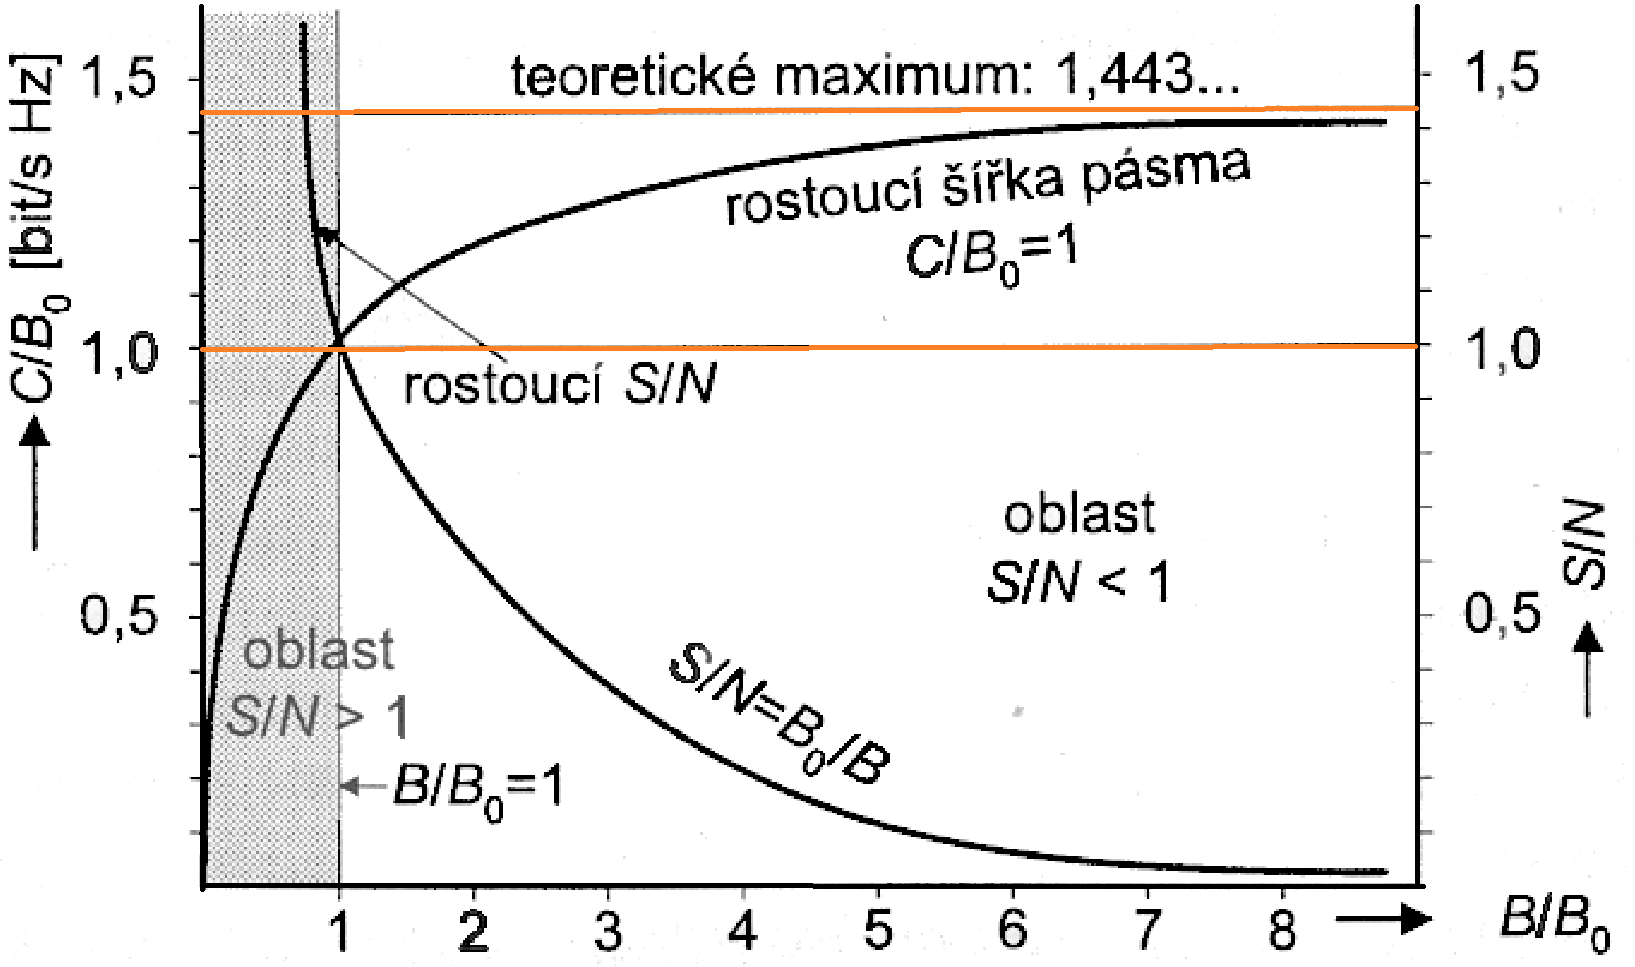
\includegraphics[width=0.8\linewidth]{shannon_graf_C_N.png}
        \caption{Závislost normované přenosové kapacity \(C/B_0\) na poměru signál/šum - \(S/N\)  
                 rádiového komunikačního systému na normované šířce pásma \(B/B_0\)
                  \cite[s.~79]{ZaludRA}}
        \label{fig_RA:modulace02}
      \end{figure} 
      
      Normovaná šířka pásma \(B/B_0\) odpovídá stavu, kdy se výkon signálu \(S\) rovná výkonu šumu 
      \(N\). Svislice vedená bodem \(B/B_0 = 1\) na vodorovné ose potom dělí celý graf na dvě 
      části. Levá, zvýrazněná část odpovídá klasickým radiokomunikačním systémům, které pracují při 
      poměru signál/šum podstatně větším než jedna, přičemž jejich normovaná přenosová kapacita je 
      hluboko pod dosažitelným maximem \(C/B_0 = 1,443\). Pravá část pak odpovídá perspektivním 
      „širokopásmovým“ radiokomunikačním systémům, které naopak pracují při poměru signál/šum \(
      S/N\ll1\), avšak s přenosovou kapacitou blížící se dosažitelnému maximu \(\num{1.443}\). Tyto 
      systémy se označují také jako \textbf{systémy s rozprostřeným spektrem}, nebo \emph{systémy s 
      kódovým multiplexem \texttt{CDMA} (Code Division Multiple Access)}. Jejich realizace je 
      obecně podstatně složitější, než realizace systémů klasických a bez vyspělé monolitické 
      technologie by byla v praxi velmi obtížná. Na druhou stranu však mají systémy druhé kategorie 
      výhodu velice efektivního využití kmitočtového spektra, které totiž mohou sdílet s jinými 
      radiokomunikačními službami aniž by se vzájemně rušily. Mezi jejich další hlavní přednosti 
      náleží možnost dobře pracovat v radiokomunikačních kanálech s vysokou úrovní poruch nebo i 
      úmyslného rušení, dále schopnost účinně potlačovat úniky signálu a konečně i schopnost 
      poměrně spolehlivě utajit přenos před nepovolanými subjekty.\cite[s.~78]{ZaludRA}
     
      
  \section{Modulace a jejich klasifikace}
    V rádiové komunikaci se používá větší počet různých typů (formátů) modulací. Jejich základní 
    klasifikace, vycházející z časového vývoje, je uvedena na obr \ref{fig_RA:modulace03}. Vývojově 
    nejstarší jsou \emph{analogové modulace}. Později se začaly uplatňovat i \emph{diskrétní 
    modulace}, a to nejprve v základním pásmu a potom i v oblasti vysokofrekvenční. Diskrétní 
    modulace v základním pásmu byly nejprve \emph{nekódované}, za nimi potom následovaly i modulace 
    \emph{kódované}. Nejmladší jsou potom \emph{diskrétní modulace s nosnými vlnami}, které pro 
    stručnost dále nazýváme \emph{modulace digitální}. Uveďme si podrobnější klasifikaci všech 
    zmíněných variant. \cite[s.~82]{ZaludRA}
    \begin{figure}[ht!]  % \ref{fig_RA:modulace03}
      \centering
      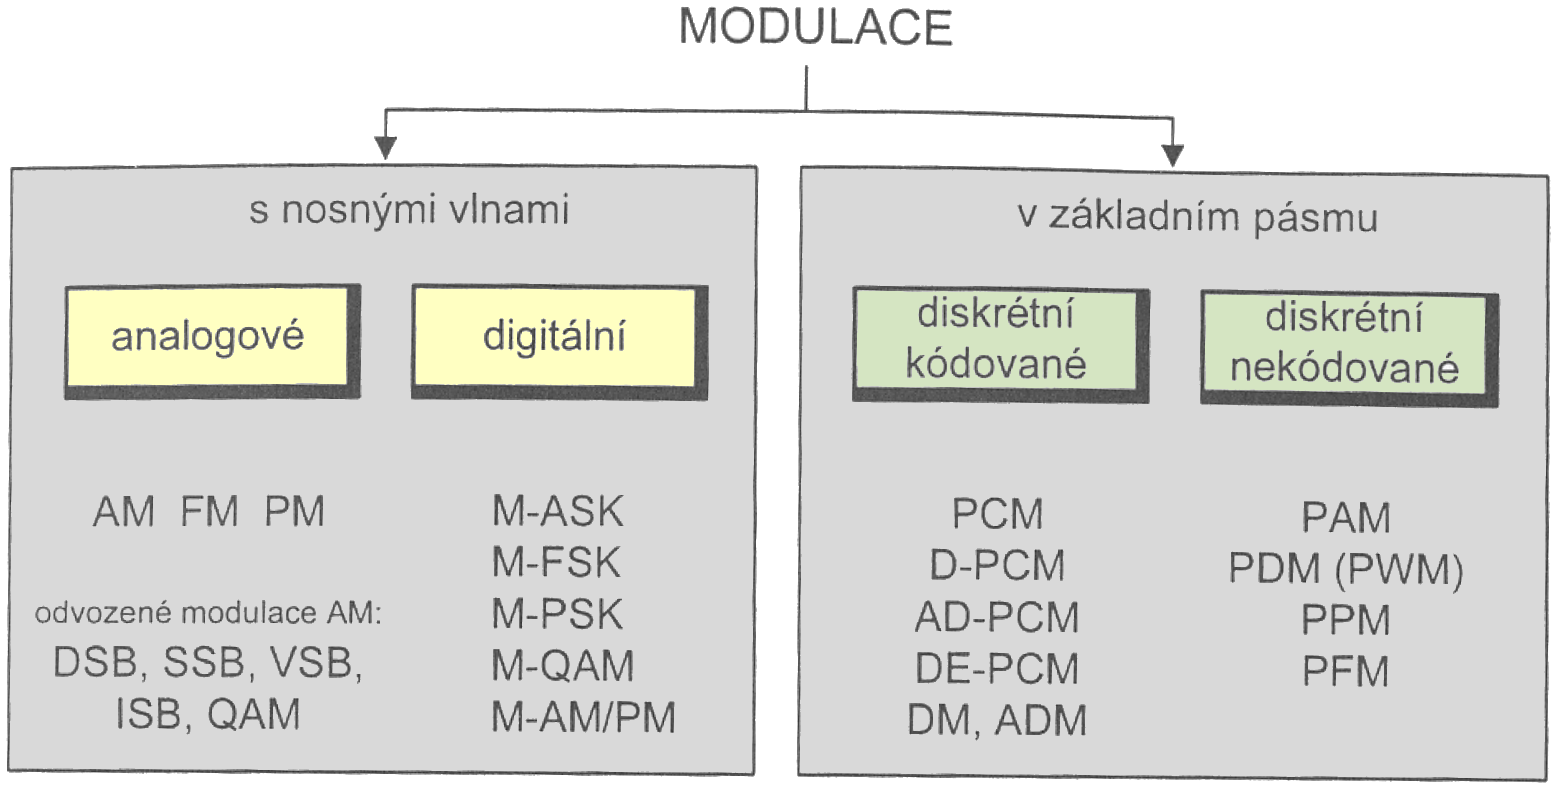
\includegraphics[width=0.9\linewidth]{modulace_prehled.png}
      \caption{Přehled modulačních způsobů používaných v rádiové komunikaci
                \cite[s.~82]{ZaludRA}}
      \label{fig_RA:modulace03}
    \end{figure}
    
    \subsection{Klasifikace analogových modulací}
      Analogové modulace vznikají tak, že se pomocí analogového modulačního signálu (tedy signálu 
      spojitého v čase i v amplitudě) moduluje analogová sinusová vysokofrekvenční nebo mikrovlnná 
      nosná vlna. Modulací se přitom rozumí ovlivňování některého parametru (charakteristické 
      veličiny) nosné vlny modulačním signálem. Je-li to amplituda, vznikne \emph{amplitudová 
      modulace \texttt{AM} (Amplitude Modulation)}, při ovlivňování kmitočtu se vytváří 
      \emph{kmitočtová modulace \texttt{FM} (Frequency Modulation)} a při ovlivňování fáze se 
      vytváří \emph{fázová modulace \texttt{PM} (Phase Modulation)}.
      
      Amplitudově modulovaný signál má kmitočtové spektrum, obsahující nemodulovanou nosnou vlnu a 
      dvě postranní kmitočtová pásma, nesoucí informaci. Určitými modifikacemi tohoto spektra potom 
      vznikají různé vývojově mladší varianty amplitudové modulace \texttt{AM}. 
      \begin{itemize}
        \item \emph{\texttt{AM} s oběma postranními pásmy \texttt{DSB} (Double Side Band)}: jsou 
               přenášena obě postranní pásma, avšak nosná je částečně nebo zcela potlačena,
        \item \emph{\texttt{AM} s jedním potlačeným postranním pásmem \texttt{SSB} (Single Side 
               Band)}: přenos jediného postranního pásma a úplně, nebo alespoň částečně potlačené 
               nosné vlna
        \item \emph{\texttt{AM} s jedním částečně potlačeným postranním pásmem \texttt{VSB} 
               (Vestigial Side Band)}: přenosu jednoho kompletního a jednoho částečně potlačeného 
               postranního pásma. Má obvykle nepotlačenou nosnou vlnu 
        \item \emph{\texttt{AM} s nezávislými postranními pásmy \texttt{ISB} (Independent Side 
               Band)}:Nosná vlna zcela nebo částečně potlačena a v každém úplném postranním pásmu 
               se přenáší nezávislý modulační signál.
        \item \emph{Analogová kvadraturní amplitudová modulace \texttt{QAM} (Quadrature Amplitudě 
               Modulation)}: používá dvě nosné vlny, které mají přesně shodné kmitočty, avšak 
               jejich fázový posuv je trvale \SI{90}{\degreeCelsius}. Každá z těchto nosných vln je 
               amplitudově modulována nezávislým modulačním signálem, přičemž může být částečně 
               nebo zcela potlačena.
      \end{itemize}
      
      Má-li být u předchozích modulací zdůrazněno, že je u nich zcela potlačena nosná vlna, bývá 
      jejich označení ještě doplněno zkratkou \emph{\texttt{SC} (Supressed Carrier)}, tedy 
      například \texttt{DSB-SC}, \texttt{SC-DSB}, nebo \texttt{DSB\textsubscript{SC}}.
      
    \subsection{Diskrétní nekódované modulace v základním pásmu}
      Základním typem této kategorie je \emph{pulzní amplitudová modulace \texttt{PAM} (Pulse 
      Amplitude Modulation)}. Ta vzniká ve své nejjednodušší podobě tak, že se analogový modulační 
      signál přivádí na klíčovaný spínač, který je spínán sledem pravoúhlých impulzů. Za spínačem 
      se potom již objevuje signál \texttt{PAM}, a to v podobě sekvence v čase nespojitých impulzů, 
      jejichž amplitudy kopírují průběh analogového modulačního signálu \cite[s.~84]{ZaludRA}.
      
      Kromě změn amplitudy se u impulzové nosné vlny dají měnit i jiné parametry viz obr. 
      \ref{fig_RA:modulace04}:
      \begin{itemize}
        \item \emph{diskrétní šířková modulace \texttt{PDM}, resp. \texttt{PWM} (Pulse Duration  
              Modulation resp. Pulse Width Modulation)}: změnou šířky impulzů impulzové nosné vlny,
        \item \emph{diskrétní polohová modulace \texttt{PPM} (Pulse Position Modulation)}: změnou  
              polohy impulzů uvažované impulzové nosné vlny, vůči poloze nominální
        \item \emph{diskrétní kmitočtová modulace \texttt{PFM} (Pulse Frequency Modulation)}:  
              změnou kmitočtu této nosné.
      \end{itemize} 
    \subsection{Diskrétní kódované modulace v základním pásmu}
      Nejrozšířenějším typem z této kategorie je \emph{impulzová kódovaná modulace \texttt{PCM} 
      (Pulse Code Modulation)}. Ta se vytváří tak, že se analogový modulační signál nejprve přemění 
      na signál \texttt{PAM}. Ten se poté podrobuje \emph{kvantování}; přitom se jeho celý 
      dynamický rozsah rozdělí na konečný počet \emph{kvantizačních úrovní (hladin)} a každé 
      skutečné úrovni impulzu \texttt{PAM} se přiřadí určitá (například nejbližší) úroveň 
      kvantizační (diskrétní). Kvantovaný signál \texttt{PAM} se dále kóduje. Kódováním se rozumí 
      převod (mapování) jeho skutečné velikosti - vyjádřené obvykle v desítkové soustavě - do 
      soustavy binární (nebo jiné, mající nižší číselný základ, než původní soustava desítková). 
      Tím se vytvoří signál s modulací \texttt{PCM}.
      \begin{itemize}
        \item \emph{diferenční \texttt{D-PCM} (Differentially - \texttt{PCM})}: nekóduje se 
              skutečná velikost kvantovaných vzorků PAM, nýbrž pouze rozdíl mezi touto skutečnou 
              velikostí a velikostí predikovanou (tj. předpověděnou z několika předchozích 
              kvantovaných vzorků).
        \item \emph{diferenciálně kódované \texttt{DE-PCM} (Differentially encoded -
              \texttt{PCM})}: nejprve se vytváří signál \texttt{PCM}; z něho se potom pomocí 
              vhodného algoritmu získává signál \texttt{DE-PCM}, u něhož je informace obsažena 
              nikoliv v samotné logické hodnotě příslušného bitu signálu \texttt{PCM}, nýbrž v 
              rozdílu tohoto bitu oproti hodnotě bitu předchozího.
        \item \emph{delta modulace \texttt{DM} (Delta Modulation)}: v podstatě představuje   
              jednobitovou variantu modulace \texttt{PCM}; je-li \(w\)-tý vzorek analogového 
              modulačního signálu větší než vzorek předchozí, je v signálu \texttt{DM} bit \(1\) a 
              je-li tento vzorek menší než předchozí, je v signálu \texttt{DM} bit \(0\).
      \end{itemize}
      
      Všechny předchozí varianty diskrétních kódovaných modulací pracují s konstantním kvantizačním 
      krokem. U \emph{adaptivní modulace \texttt{D-PCM} tj. \texttt{AD-PCM}} a rovněž u 
      \emph{adaptivní modulace \texttt{DM} tj. \texttt{A-DM}}, se kvantizační krok naopak mění v 
      závislosti na průběhu analogového modulačního signálu.
    
    \begin{figure}[ht!]  % \ref{fig_RA:modulace04}
      \centering
      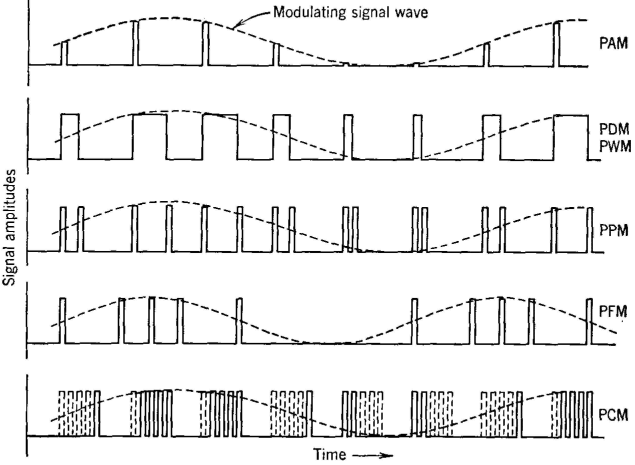
\includegraphics[width=1\linewidth]{modulace_zakladni_pasmo.png}
      \caption{Přibližné tvary a uspořádání signálů diskrétních pulsní modulací pro sinusový   
               modulační signál (tečkovaná křivka). Výška impulsů obecně neodpovídá výšce modulační 
               vlny.}
      \label{fig_RA:modulace04}
    \end{figure}
    
    \subsection{Digitální modulace (diskrétní modulace s nosnými vlnami)}
      Tyto modulace vznikají tak, že se vysokofrekvenční nebo mikrovlnná sinusová nosná vlna 
      moduluje signálem některé diskrétní modulace v základním pásmu; jedná se zde tedy vlastně o 
      dvojnásobnou modulaci, neboť modulačním signálem je již předtím modulovaný signál. K modulaci 
      se používá většinou binární signál \texttt{PCM}, nebo jeho některé modifikace, ostatní 
      diskrétní modulace se k danému účelu používají jen zřídka.
      
      Binárním modulačním signálem je možné modulovat amplitudu, kmitočet anebo fázi nosné vlny. U 
      \emph{dvoustavových modulací} se modulovaný parametr této vlny mění pouze mezi dvěma 
      diskrétními stavy, z nichž jeden odpovídá modulačnímu bitu 0 a druhý bitu 1. Tyto diskrétní 
      stavy nosné vlny se u digitálních modulací označují obecně termínem \emph{signálové prvky} 
      resp. \emph{symboly}, okamžiky přechodu mezi nimi se potom nazývají \emph{charakteristické 
      okamžiky}. Pro uvažované digitální modulace se používá rovněž termín \textbf{klíčování}; 
      (změny nosné vlny mezi několika diskrétními stavy se tímto slovem označují vlastně již od 
      počátků radiokomunikace, nejprve zřejmě ve spojení „klíčovaná telegrafie“).
      \begin{itemize}
        \item \emph{dvoustavové klíčování amplitudovým zdvihem \texttt{2-ASK} (Amplitudě Shift  
              Keying)}: klíčováním amplitudy nosné vlny, se získá dvoustavová modulace 
              \texttt{PCM-AM}
        \item \emph{dvoustavové klíčování kmitočtovým zdvihem \texttt{2-FSK} (Frequency Shift  
              Keying)}: klíčování kmitočtu nosné vlny se vytváří dvoustavová modulace 
              \texttt{PCM-FM},
        \item \emph{dvoustavové klíčování fázovým zdvihem \texttt{2-PSK}, (Phase Shift Keying)}: 
              klíčování fáze nosné vlny potom konečně vzniká dvoustavová modulace \texttt{PCM-PM}.
      \end{itemize}
      U dvoustavových modulací odpovídá každý modulační stav modulované nosné vlny jedinému bitu 
      modulačního signálu \texttt{PCM}. Snaha po zvětšení přenosové kapacity digitálních modulací 
      však vedla k rychlému rozvoji \emph{vícestavových diskrétních modulací}, u nichž každý 
      signálový prvek modulované nosné vlny přenáší nejméně dva, nebo i více bitů. Tak například u 
      \emph{čtyřstavové modulace \texttt{4-FSK (Q-FSK)}} tato vlna zaujímá čtyři diskrétní 
      kmitočty; každá z nich zde však již nereprezentuje jediný bit jako v případě modulace 
      \texttt{2-FSK}, nýbrž dva bity, tj. \emph{bitovou dvojici}, nazývanou také \emph{dibit}. 
      Analogicky   \emph{čtyřstavová modulace \texttt{4-PSK (Q-PSK)}} pracuje se čtyřmi diskrétními 
      fázovými 
      stavy nosné vlny, z nichž každý odpovídá určitému dibitu modulačního signálu atd. Rychlost, 
      se kterou se mění diskrétní stavy nosné vlny se nazývá \textbf{symbolová rychlost} \(f_s\) 
      tato rychlost se vyjadřuje v jednotkách \emph{baud \textbf{[Bd]}}, přičemž je rovna reciproké 
      hodnotě doby trvání \(T_s\) signálového prvku, tedy\[f_s = \frac{1}{T_s}.\]
      
      U čtyřstavových modulací \texttt{4-ASK}, \texttt{4-FSK} a \texttt{4-PSK} zřejmě každý 
      signálový prvek přenáší dva bity, proto je zde symbolová rychlost \(f_s\) rovna právě jedné 
      polovině bitové rychlosti \(f_b\) V důsledku toho je potom i potřebná šířka pásma 
      vy\-so\-ko\-frek\-ven\-ční\-ho kanálu u těchto modulací poloviční, v porovnání s modulacemi 
      dvoustavovými (ovšem při téže bitové rychlosti modulačního signálu \texttt{PCM}). U 
      osmistavových modulací nese každý signálový prvek informaci již o třech bitech (tj. o jednom 
      \textbf{tribitu}), což vede pouze ke třetinové šířce pásma vysokofrekvenčního kanálu. Obecně 
      potom platí, že u modulace s \(M\) stavy přenáší každý symbol informaci o \(n = \log_2 M\) 
      bitech. Šířka pásma \(B_M\) kanálu obecné \emph{M-stavové modulace}, v závislosti na šířce 
      pásma \(B_2\) základní dvoustavové modulace, je tedy určena vztahem \(B_M = \frac{B_2}{\log_2 
      M}.\) 
      
      Vývojově mladší kategorii digitálních modulací potom představují \emph{M-stavové modulace se 
      současným klíčováním amplitudy a fáze nosné vlny}, značené původně symbolem 
      \texttt{M-ASK/PSK}; pro tyto modulace je však již běžnější označení \emph{M-stavové 
      kvadraturní amplitudové modulace \texttt{M-QAM}\footnote{nezaměňovat s analogovou kvadraturní 
      modulací \texttt{QAM}, popisovanou výše} (Quadrature Amplitude Modulation)}.
      
      Od počátku devadesátých let se dostávají do praxe také již zmíněné \emph{kódované modulace}, 
      které vznikají spojením kanálového kódování a vlastní modulace do jediného procesu, 
      realizovaného v jediném funkčním bloku. 
    
    \subsection{Lineární modulace a nelineární modulace, modulace s pamětí a bez paměti}
      Předchozí klasifikace modulací vychází z jejich historického vývoje, přičemž rozlišuje 
      jednotlivé modulace na základě různých typů modulačních signálů a rozdílných modulovaných 
      parametrů nosné vlny.
      
      Dělení na \textbf{lineární} a \textbf{nelineární modulace} se uplatňuje především u modulací 
      s nosnými vlnami. \emph{Analogové lineární modulace} jsou takové, u nichž je amplituda nosné 
      vlny danou, obecně lineární funkcí okamžitých hodnot modulačního signálu. U lineárních 
      modulací Platí \emph{princip superpozice} mezi různými složkami kmitočtového spektra 
      modulovaného signálu, příslušejícími různým složkám spektra modulačního signálu. Do této 
      kategorie patří amplitudová modulace AM i všechny její varianty, tj. modulace \texttt{DSB}, 
      \texttt{SSD} atd. U \emph{analogových nelineárních modulací} zmíněná lineární závislost 
      amplitudy nosné na modulačním signálu neexistuje a princip superpozice neplatí, takže ve 
      spektru modulovaného 
      signálu jsou přítomny také \emph{intermodulační produkty} základních složek. Sem náležejí dvě 
      kategorie tzv. \emph{exponenciálních modulací}, a to \emph{kmitočtová modulace \texttt{FM}} a 
      \emph{fázová modulace \texttt{PM}}; tyto modulace jsou charakterizovány \emph{konstantní 
      obálkou nosné vlny}. U \emph{diskrétních lineárních modulací} při mapování modulačního 
      digitálního signálu (informační datové sekvence), do po sobě následujících stavů (signálových 
      prvků) modulované nosné vlny, platí princip superpozice. U \emph{diskrétních nelineárních 
      modulací} naopak princip superpozice mezi po sobě následujícími stavy modulovaného signálu 
      neplatí. Tyto   modulace mohou, ale také nemusí mít konstantní obálkou modulované nosné vlny, 
      v závislosti na tom zda se u nich netvaruje - nebo tvaruje modulační datová sekvence.
      
      U \textbf{digitálních modulací s pamětí} určitý stav nosné vlny závisí nejen na jemu 
      odpovídajícím bloku (kódové skupině) binárního modulačního signálu, nýbrž určitým způsobem i 
      na předchozích stavech této vlny, resp. na předchozích blocích modulačního signálu. Uvedená 
      závislost zde vzniká zpravidla již na úrovni modulačních signálů, které se totiž z původní 
      vstupní podoby nejprve překódují do podoby „s pamětí“ a teprve poté se přivádějí na 
      modulátor. U \textbf{digitálních modulací bez paměti} se tato závislost neobjevuje.
      
      Výše uvedené kategorie se mohou vzájemně kombinovat, čímž vznikají celkem čtyři možné 
      varianty, které se striktně rozlišují především u digitálních modulací. K lineárním modulacím 
      bez paměti náležejí například formáty \texttt{2-PSK, 4-PSK,} k lineárním modulacím s pamětí 
      formáty \texttt{DE-PSK, \(\pi\)/4-QPSK} atd. 
      
      Poslední klasifikace se týká pouze modulací, u nichž je modulační signál \emph{nespojitý 
      (diskrétní) v čase}. \textbf{Koherentní modulace} jsou takové, u nichž existuje předem určený 
      vztah mezi okamžiky charakterizujícími fázi nosné vlny před modulací a charakteristickými 
      okamžiky modulovaného signálu. Do této kategorie náležejí například modulace, u nichž 
      charakteristické okamžiky modulovaného signálu splývají s průchody nosné vlny nulou 
      (konkrétně je to např. modulace MSK apod.). Modulace, u nichž předem určený vztah mezi fází 
      nosné vlny a charakteristickými okamžiky modulovaného signálu neexistuje, se nazývají 
      \textbf{modulace nekoherentní}.
      
  \section{Analogové modulace}
    Vývojově nejstarší systémy pro pozemskou radiokomunikaci používaly pro přenos analogovou 
    amplitudovou modulaci \texttt{AM}, k níž se později připojila analogová kmitočtová modulace 
    \texttt{FM} a fázová modulace \texttt{PM}. Modulace \texttt{AM} a její varianty se v současné 
    době uplatňují spíše už jen u jednodušších systémů, jako je například rozhlas \texttt{AM}, 
    občanské radiostanice apod. Naproti tomu modulace \texttt{FM} stále ještě nachází využití i v 
    náročnějších aplikacích jako je stereofonní rozhlas \texttt{FM} apod \cite[s.~75]{ZaludRA}.
    
    \subsection{Základní principy analogových modulací}
      U analogových modulací se obecným modulačním signálem \(m(t)\) moduluje vhodný parametr 
      spojité, harmonické (např. kosinusové) vysokofrekvenční nosné vlny. Modulační signál může mít 
      charakter napětí nebo proudu, v dalším však většinou předpokládáme, že je to signál napěťový. 
      Modulované napětí lze potom vyjádřit obecným vztahem
      \begin{equation}\label{eq:RA_mdlc_01}
        u_{mod}(t) = u_i(t)\cos[\Phi_i(t)]
      \end{equation}
      kde \(u_i (t)\) je \emph{okamžitá amplituda} napětí modulované nosné vlny; \(\Phi_i(t)\) 
      okamžitá fáze modulované nosné vlny.
      
      Mění-li se amplituda napětí \(u_i(t)\) modulované nosné vlny lineárně s modulačním napětím 
      \(m(t)\), přičemž okamžitá fáze \(\Phi_i(t)\) zůstává konstantní, získá se \emph{amplitudová 
      modulace}, která náleží do kategorie \emph{lineárních modulací}. U lineárních modulací jsou v 
      kmitočtovém spektru modulovaného signálu obsaženy jen složky, které odpovídají jednotlivým 
      harmonickým složkám modulačního signálu.
      
      Jestliže se u modulované nosné vlny mění podle určitého zákona okamžitá fáze \(\Phi_i(t)\) s 
      modulačním napětím \(m(t)\), přičemž amplituda zůstává konstantní, vytvářejí se \emph{úhlové 
      (exponenciální) modulace}, náležející do kategorie \emph{nelineárních modulací}. V jejich 
      kmitočtovém spektru jsou nejen složky odpovídající jednotlivým harmonickým modulačního 
      signálu, nýbrž i jejich vzájemné intermodulační produkty. Z nich je nejčastěji využívána 
      \emph{kmitočtová modulace \texttt{FM}}, u níž je okamžitá odchylka kmitočtu (tj. derivace 
      fáze podle času) modulované nosné vlny, vůči kmitočtu nemodulované nosné vlny, úměrná 
      modulačnímu signálu. K exponenciálním modulacím náleží dále \emph{fázová modulace 
      \texttt{PM}}, u níž je okamžitá odchylka fáze, od fáze nemodulované nosné vlny, úměrná 
      modulačnímu signálu. Modulace \texttt{FM} a \texttt{PM} mají konstantní obálku modulované 
      nosné vlny. To je v praxi výhodné, neboť signály s konstantní obálkou mohou být zesilovány 
      výkonovými zesilovači nastavenými do nelineární pracovní třídy C (D, E, ...), vyznačující se 
      velkou energetickou účinností, okolo \num{50} až \num{80}\%.
      
    \subsection{Amplitudová modulace AM}
      Základním typem amplitudových modulací je \emph{amplitudová modulace s oběma postranními 
      pásmy a nepotlačenou nosnou vlnou}, značená symbolem \emph{\texttt{AM} (Amplitude 
      Modulation)}. Její podstatu ukazuje obr. \ref{fig_RA:modulace05}. Na obr. 
      \ref{fig_RA:modulace06} je znázorněn časový průběh modulačního signálu \(m(t)\), o němž 
      nejprve pro jednoduchost předpokládejme, že je kosinusový (harmonický) a má amplitudu 
      \(U_m\) a kmitočet \(f_m\). Na obr. \ref{fig_RA:modulace07} je znázorněna kosinusová nosná 
      vlna \(u_c(t)\) o amplitudě \(Uc\) a kmitočtu \(f_c\). Tyto průběhy lze vyjádřit relacemi
      \begin{equation}\label{eq:RA_mdlc_02}
        m(t) = U_m(t)\cos(2\pi f_m t); \qquad u_c(t) = U_c(t)\cos(2\pi f_c t)
      \end{equation}

      \begin{figure}[ht!]
        \centering
        \subcaptionbox{harmonický (kosinusový) modulační signál \(m(t)\) \label{fig_RA:modulace05}}
          {\luafigure[0.8]{modulace05_AM.png}}              \newline
        \subcaptionbox{harmonická (kosinusová) nosná vlna \(u_c(t)\)     \label{fig_RA:modulace06}}
         {\luafigure[0.8]{modulace06_AM.png}}              \newline
        \subcaptionbox{odpovídající modulovaný \texttt{AM} signál  
                  \(u_{AM}(t)\)                                          \label{fig_RA:modulace07}}
          {\luafigure[0.8]{modulace07_AM.png}}              \newline
        \subcaptionbox{kmitočtové spektrum \(F_{AM}(f)\) signálu AM při obecném, neharmonickém  
                  modulačním signálu                                     \label{fig_RA:modulace08}}
          {\luafigure[0.7]{modulace08_AM.png}}              \newline
        \subcaptionbox{fázorová reprezentace signálu \texttt{AM}.        \label{fig_RA:modulace09}}
          {\luafigure[0.7]{modulace09_AM.png}}  
        \caption{Podstata amplitudové modulace \texttt{AM}}
      \end{figure}
      
      Amplitudová modulace \texttt{AM} je definována jako modulace, při níž se amplituda nosné vlny 
      mění okolo své střední hodnoty \(U_c\) lineárně s modulačním signálem \(m(t)\). Časový průběh 
      příslušného modulovaného napětí \(u_m(t)\), znázorněného na obr. \ref{fig_RA:modulace07} je 
      tedy dán relací
    
%--------------------------------------------------------------------------------------------------- 
}
{
% DEBUG was off
%=====================================Kapitola: Hlavní etapy vývoje fyziky==========================
%  % !TeX spellcheck = cs_CZ
\sisetup{input-complex-roots = j, 
         output-complex-root = \ensuremath{\mathrm{j}}}
         
%==================Kapitola: Teoretické základy radioelektroniky====================================
\chapter{Teoretické základy radioelektroniky}\label{chap:ra_theory}
\minitoc
  %--------------- Úvod do šíření vln pro pozemní rádiové spoje ------------------------------------
  \section{Úvod do šíření vln pro pozemní rádiové spoje}
    \begin{example}
      Domácí meteostanice používá pro komunikaci s externím čidlem na měření vnější teploty 
      frekvenci \SI{433}{MHz}. Určete délku vln a rádiové pásmo do kterého použitá vlnová délka 
      patří.
      \newline\textbf{řešení:}
      \begin{equation}
        \lambda = c\cdot T = \frac{c}{f} = \frac{\num{300e6}}{\num{433e6}} = \SI{0.49}{\meter}
      \end{equation}
      Domácí meteostanice používá pro komunikaci s čidlem ultrakrátké vlny o vlnové délce 
      \SI{0.49}{\meter} 
    \end{example}
    
  %--------------- Základní klasifikace radioelektronických systémů --------------------------------
  \section{Základní klasifikace radioelektronických systémů}
    Pod pojmem systém \cite[s.~56]{ZaludRA} 

  \section{Dvojbrany v radioelektronice}
    Pod pojmem \emph{systém} se zde označuje elektrický obvod nebo soustava obvodů, které vytvářejí 
    alespoň jeden výstupní signál jako odezvu na alespoň jeden vstupní signál. Jednou z 
    nejdůležitějších tříd radioelektronických systémů jsou lineární systémy s časově invariantními 
    (neměnnými) parametry, které mají podobu \emph{n-branů}. Mezi nimi potom zaujímají významné 
    místo lineární dvojbrany a trojbrany, jejichž popisem a obecnými vlastnostmi se zabývá tato 
    kapitola. Připomeňme, že pro označení linearity a časové invariance se v teorii obvodů používá 
    zkratka \emph{LTI- (Linear Time Invariant)}, což nijak dále nezdůrazňujeme, nebo tato kapitola 
    je zaměřena právě jen na dvojbrany a trojbrany tohoto typu.
    
    V radioelektronice se často vyskytují dvojbrany a trojbrany, které přísně vzato lineární 
    nejsou, avšak jejich nelinearity jsou tak malé, že je lze v technické praxi zanedbat; do této 
    kategorie patří například všechny obvody s diodami a s tranzistory, pracujícími v režimu malých 
    signálů, kde jsou prakticky lineární a nelinearity se u nich začínají projevovat až při vyšších 
    úrovních signálů. Tyto dvojbrany a trojbrany, označované termínem kvazilineární (tedy téměř 
    lineární) Jsou rovněž zahrnuty do této kapitoly. Zvláštní pozornost je věnována zejména jejich 
    vlastnostem v hraniční oblasti mezi lineárním a nelineárním režimem, která je v 
    radioelektronice velmi důležitá.
    
    \subsection{Admitanční parametry a rozptylové parametry dvojbranů}
      Pod pojmem dvojbran (\emph{two-port}) se rozumí elektrický systém, který má jeden pár 
      vstupních svorek a jeden pár výstupních svorek, tedy jednu vstupní a jednu výstupní bránu 
      (dvojbran zřejmě představuje zvláštní třídu obecnějšího pojmu \emph{čtyřpól}, který má čtyři 
      nezávislé svorky). Linearizované přenosové vlastnosti dvojbranů je možné charakterizovat 
      pomocí jejich \textbf{admitančních} a \textbf{rozptylových parametrů}, kterým je dále 
      věnována náležitá pozornost \cite[s.~331]{ZaludRA}.
      
      Při definici \emph{admitančních parametrů} dvojbranů, nazývaných také parametry \(y\) 
      \emph{(Admittance Parameters)}, vyjdeme z obr. \ref{RA:fig_dvojbran01}. Zde je znázorněn 
      lineární časově invariantní dvojbran, který má na vstupu svorkové napětí a proud \(u_l\), 
      \(i_1\) a na výstupu \(u_2\), \(i_2\). K jeho vstupu je připojen generátor s vnitřní 
      admitancí \(Y_g\) a k výstupu zatěžovací admitance \(Y_z\). Admitanční parametry tohoto 
      dvojbranů jsou definovány relacemi
      \begin{align}
        i_1 &= y_{11}u_1 + y_{12}u_2   \\ 
        i_2 &= y_{21}u_1 + y_{22}u_2
      \end{align}
      
      \begin{figure}[ht!]
        \centering  
        \begin{tabular}{cc}
          \subfloat[ ]{\label{RA:fig_dvojbran01}
            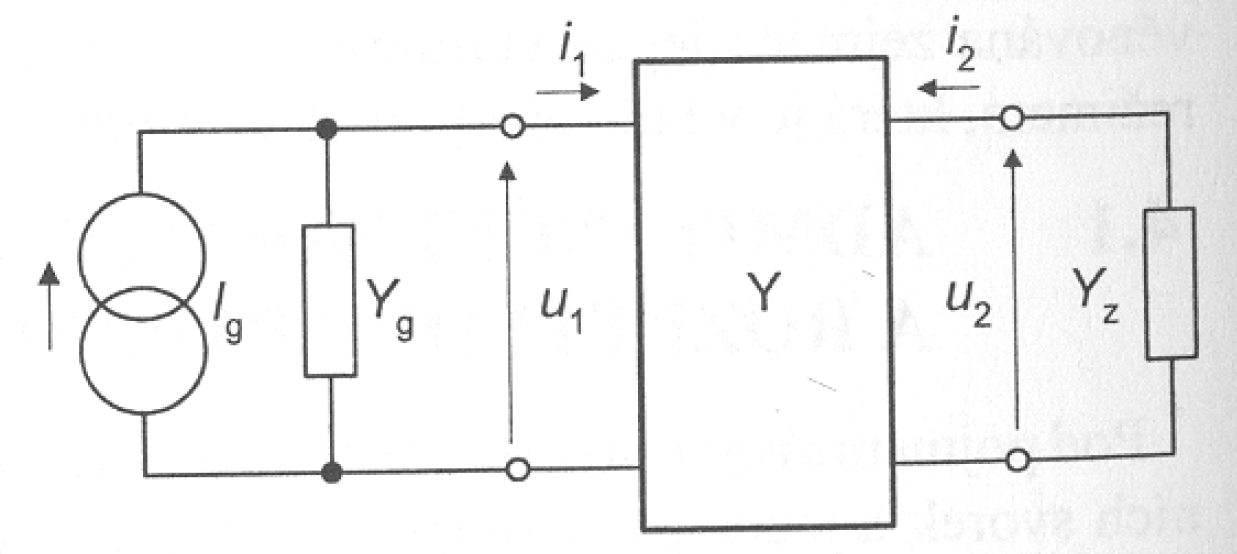
\includegraphics[width=0.4\linewidth]{RA_dvojbran01.png}}              &
          \subfloat[ ]{\label{RA:fig_dvojbran02}
            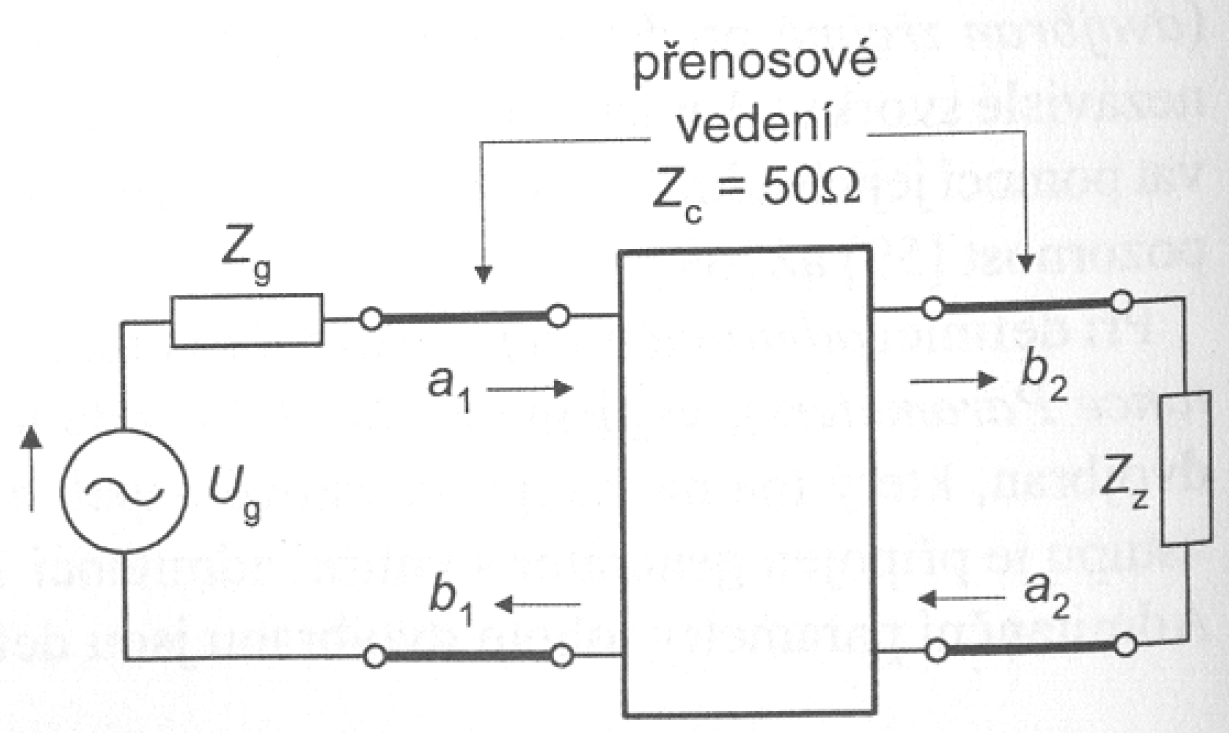
\includegraphics[width=0.4\linewidth]{RA_dvojbran02.png}}              \\
        \end{tabular}
        \caption{Charakterizace dvojbranu: a) svorkovými napětími a proudy; 
                 b) dopadajícímí a odraženými napěťovými vlnami}\label{RA:fig_dvojbran}
      \end{figure}
      
      Z těchto vztahů vyplývá, že admitance \(y_{11}\) je rovna \emph{vstupní admitanci dvojbranu} 
      při jeho výstupu nakrátko (\(u_2=0\)), a podobně admitance \(y_{22}\) je \emph{výstupní 
      admitance} při vstupu nakrátko (\(u_1=0\)). Admitance \(y_{21}\), resp. \(y_{12}\) je potom 
      \emph{přenosová admitance} v předním nebo zpětném směru, při výstupu resp. vstupu nakrátko.
      
      Jak je patrné, parametry \(y\) jsou definovány při vstupu nebo výstupu nakrátko. Při jejich 
      měření však lze tuto podmínku splnit bez potíží jen při nižších kmitočtech, nepřesahujících 
      asi 300 MHz. Ve vyšších pásmech je možné vytvořit „zkrat“ např. vyladěným sériovým 
      rezonančním obvodem, nebo transformačním členem složeným z obvodů s rozloženými parametry, 
      což však příliš komplikuje měření (velké potíže vznikají zejména při návrhu širokopásmových 
      automatizovaných měřičů parametrů \(y\) s rozmítaným kmitočtem, které jsou v mikrovlnném 
      pásmu prakticky nerealizovatelné). Z tohoto, ale i z dalších důvodů byla během šedesátých let 
      propracována nová soustava parametrů označovaných jako parametry \(s\), nebo 
      \textbf{parametry rozptylové} (\emph{Scattering Parameters}). Definice rozptylových parametrů 
      dvojbranů vychází z obr. \ref{RA:fig_dvojbran02}. Zde je opět znázorněn lineární, časově 
      invariantní dvojbran, avšak jeho vlastnosti již nejsou charakterizovány svorkovými napětími a 
      proudy, ale \emph{normovanými dopadajícími napěťovými vlnami} \(a_1, a_2\) a \emph{odraženými 
      napěťovými vlnami} \(b_1, b_2\). Tyto vlny se vytvářejí na vstupním a na výstupním přenosovém 
      vedení o charakteristické impedanci \(Z_c\). Svorková napětí a proudy jsou vázány s 
      napěťovými vlnami jednoduchými vztahy
      \begin{align}\label{RA:eq_01}
      u_1 &= (a_1 + b_1)\cdot\sqrt{Z_c} \qquad i_1 = \frac{a_1-b_1}{\sqrt{Z_c}}   \\ 
      u_2 &= (a_2 + b_2)\cdot\sqrt{Z_c} \qquad i_1 = \frac{a_2-b_2}{\sqrt{Z_c}}
      \end{align}
      
      Naopak dopadající a odražené vlny jsou v závislosti na svorkových napětích a proudech určeny 
      vztahy
      \begin{align}\label{RA:eq_02}
      a_1 &= \frac{u_1 + i_1Z_c}{2\sqrt{Z_c}} \qquad b_1 = \frac{u_1 - i_1Z_c}{2\sqrt{Z_c}}   \\ 
      a_2 &= \frac{u_2 + i_2Z_c}{2\sqrt{Z_c}} \qquad b_1 = \frac{u_2 - i_2Z_c}{2\sqrt{Z_c}}
      \end{align}
      
      \emph{Charakteristická impedance} \(Z_c\), nazývaná v této souvislosti také \emph{impedancí 
      vztažnou (referenční)}, může obecně být komplexní veličinou; dále však předpokládejme, že je 
      reálná, stejná pro vstupní i výstupní bránu, s typickou hodnotou \(Z_c = \SI{50}{\ohm}\) (v 
      praxi se používají ještě impedance \SI{60}{\ohm} a \SI{75}{\ohm}). Vzájemnou závislost 
      dopadajících a odražených napěťových vln vyjadřují relace
      \begin{align}\label{RA:eq_03}
      b_1 &= s_{11}a_1 + s_{12}a_2   \\ 
      b_2 &= s_{21}a_1 + s_{22}a_2
      \end{align}
      které lze považovat za definiční vztahy rozptylových parametrů daného dvojbranu. Z nich se 
      snadno odvodí fyzikální význam jednotlivých parametrů:
      \begin{itemize}
        \item \textbf{vstupní napěťový činitel odrazu}, při výstupu zakončeném zátěží \(Z_z\), 
              přizpůsobenou k vztažné impedanci \(Z_c\)  (tj. \(Z_z = Z_c\) a tedy \(a_2 = 0\)):
              \begin{equation*}
                s_{11} = \left(\dfrac{b_1}{a_1}\right)_{a_2=0}
              \end{equation*}
        \item \textbf{výstupní napěťový činitel odrazu}, při vstupu zakončeném impedancí \(Z_g\), 
               přizpůsobenou k vztažné impedanci \(Z_c\) (tj. \(Z_g = Z_c\) a tedy \(a_1 = 0\)); 
              \begin{equation*}
                 s_{22} = \left(\dfrac{b_2}{a_2}\right)_{a_1=0}
              \end{equation*}
        \item \textbf{vložné napěťové zesílení v předním směru}, při výstupu zakončeném zátěží 
              \(Z_z\), přizpůsobenou k vztažné impedanci \(Z_c\) (tj. \(Z_z = Z_c\) a tedy \(a_2 = 
              0\));
              \begin{equation*}
                 s_{12} = \left(\dfrac{b_1}{a_2}\right)_{a_1=0}
              \end{equation*}
        \item \textbf{vložné napěťové zesílení v závěrném směru}, při vstupu zakončeném impedancí 
              \(Z_g\), přizpůsobenou k vztažné impedanci \(Z_c\) (tj.\(Z_g = Z_c\) a tedy \(a_1 = 
              0\)); \\
              \begin{equation*}
                 s_{12} = \left(\dfrac{b_1}{a_2}\right)_{a_1=0}
              \end{equation*}
      \end{itemize}
      
      Takto definované parametry \(s\) jsou závislé na impedanci \(Z_c\), proto jejich číselné 
      hodnoty je třeba vždy doplnit údajem o její hodnotě. Při grafickém znázornění se parametry 
      \(s_{11}\) a \(s_{22}\), představující \emph{činitele odrazu}, zakreslují obvykle do 
      příslušného rastru \emph{Smithova diagramu}; parametry \(s_{12}\) a \(s_{21}\) se potom 
      zobrazují do komplexní roviny, nejčastěji v polárním tvaru.
        
      V předchozích úvahách jsou rozptylové parametry definovány pomocí normovaných napěťových vln 
      \(a\), \(b\). Kvadráty modulů těchto vln \(a_2\) resp. \(b_2\) jsou rovny dopadajícím resp. 
      odraženým výkonům na vstupu a na výstupu dvojbranu. Proto se vlny \(a\), \(b\) označují také 
      jako výkonové vlny, ačkoliv přesněji vzato vyjadřují odmocniny z příslušných výkonů.
        
      Nehledě na to, že parametry \(y\) jsou definovány pomocí svorkových napětí a proudů a 
      parametry \(s\) pomocí dopadajících a odražených vln, existují mezi nimi vzájemné jednoznačné 
      vztahy. Tak např. parametr \(y_{11}\) definovaný pro \(u_2 = 0\), tj. pro 
      \(\dfrac{a_2}{b_2}=-1\), lze se zřetelem na převodní vztahy (\ref{RA:eq_01}), 
      (\ref{RA:eq_02}) vyjádřit ve tvaru
      \begin{equation}\label{RA:eq_04}
        y_{11} = \left(\frac{i_1}{u_1}\right)_{u_{22}} = \frac{a_1-b_1}{Z_c(a_1+b_1)} = 
                 \frac{1-\dfrac{b_1}{a_1}}{Z_c1+\left(\dfrac{b_1}{a_1}\right)} 
      \end{equation}
      Z definičních vztahů (\ref{RA:eq_03}) však plyne, že \(\frac{b_1}{a_1} = (\det s + s_{11})(1 
      + s_{22})\), kde \(\det s = s_{11}s_{22} -s_{21}s_{l2}\). Dosazením poslední relace do 
      (\ref{RA:eq_04}) se tedy získá převodní vztah
      \begin{equation}
        y_{11} = \frac{(1+s_{22})(1-s_{11})+s_{12}s_{21}}{(1+s_{11})(1+s_{22})-s_{12}s_{21}}
      \end{equation}
      
    \subsection{Vektorové měření impedance a přizpůsobení}
      \subsubsection{Činitel odrazu, přepočet na impedanci, poměr stojatého vlnění}
        Komplexní činitel odrazu \(\Gamma_L\) zátěže o impedanci \(Z_L\) připojené na konec 
        homogenního vedení o vlnové impedanci \(Z_0\) je v rovině připojení impedance \(Z_L\) 
        definován jako poměr fázoru harmonické napěťové vlny \(U^-\) na svorkách zátěže \(Z_L\), 
        která se od této zátěže odráží (odražená vlna), ku fázoru napěťové vlny \(U^+\) na svorkách 
        zátěže \(Z_L\), která na zátěži \(Z_L\) přichází po vedení (postupná vlna), tj.
        \begin{equation}\label{RA:eq_smith01}
          \Gamma_L = \frac{U^-}{U^+}
        \end{equation}
        Činitel odrazu je v této rovině funkcí pouze \(Z_0\) a \(Z_L\), přičemž obě tyto impedance 
        mohou být kmitočtově závislé (a také bývají, zejména \(Z_L\)).
  
        Mezi činitelem odrazu \(\Gamma_L\) a impedancemi \(Z_0\) a \(Z_L\) lze odvodit vztah
        \begin{equation}\label{RA:eq_smith02}
          \Gamma_L = \frac{Z_L-Z_0}{Z_L-Z_0}.
        \end{equation}    
        Pokud známe vlnovou impedanci vedení \(Z_0\) a činitel odrazu \(\Gamma_L\), lze ze vztahu 
        \ref{RA:eq_smith02} snadno vyjádřit zatěžovací impedanci \(Z_L\)
        \begin{equation}\label{RA:eq_smith03}
          Z_L = Z_0\frac{1+\Gamma_L}{1-\Gamma_L},
        \end{equation}    
  
        často udávaným parametrem popisujícím míru nepřizpůsobení je poměr stojatého vlnění – 
        \textbf{PSV} \emph{(Voltage Standing Wave Ratio – VSWR)}. Je definován jako poměr maximální 
        a minimální hodnoty amplitudy tzv. stojatého vlnění, které vzniká součtem postupné a 
        odražené vlny na vedení. Poměr stojatého vlnění lze vyjádřit taktéž pomocí vlnové impedance 
        vedení \(Z_0\) a zatěžovací impedance \(Z_L\), a tedy i pomocí činitele odrazu \(\Gamma_L\)
        \begin{equation}\label{RA:eq_smith04}
          PSV = \frac{U_{max}}{U_{min}} 
              = \frac{\abs{Z_L+Z_0} + \abs{Z_L-Z_0}}{\abs{Z_L+Z_0} - \abs{Z_L-Z_0}} 
              = \frac{1+\abs{\Gamma_L}}{1-\abs{\Gamma_L}}.
        \end{equation}
        Poslední výraz umožňuje odpoutat definici poměru stojatého vlnění od vedení a pracovat s 
        ním podobně jako s velikostí činitele odrazu \(\Gamma_L\).
      
      \subsubsection{Impedanční přizpůsobení pomocí obvodů se soustředěnými parametry}
        Přivádíme-li vysokofrekvenční signál z generátoru o vnitřní impedanci \(Z_G\) na zátěž o 
        impedanci \(Z_L\), je obvykle žádoucí dosažení stavu tzv. \emph{impedančního přizpůsobení}. 
        Přitom rozlišujeme dva typy impedančního přizpůsobení. Prvním je \emph{impedanční 
        přizpůsobení pro maximální přenos výkonu}, pro které platí
        \begin{equation}\label{RA:eq_smith05}
          Z_L = Z^*_G,
        \end{equation}  
        kde \(Z^*_G\) je komplexně sdružená hodnota k vnitřní impedanci generátoru \(Z_G\). V tomto 
        stavu obdržíme na zátěži \(Z_L\) největší činný výkon, jaký je generátor vůbec schopen do 
        nějaké zátěže dodat – tzv. \emph{dosažitelný výkon}.
  
        Druhým typem je \emph{bezodrazové impedanční přizpůsobení}, vhodné v případě, kdy na zátěž 
        \(Z_L\) přivádíme signál po vedení o vlnové impedanci \(Z_0\) nezanedbatelné délky vzhledem 
        k vlnové délce signálu. V tomto stavu platí
        \begin{equation}\label{RA:eq_smith06}
          Z_L = Z_0,
        \end{equation}  
        a jeho výhodou je, že při něm na konci vedení nedochází k odrazům, které by jinak mohly 
        kromě zhoršení účinnosti přenosu výkonu způsobit také degradaci kvality signálu (v případě 
        odrazů na obou koncích vedení, např. tzv. „duchy“ v televizním obrazu způsobené právě 
        nepřizpůsobeným anténním napáječem). Jelikož u většiny vedení máme v praxi téměř nulovou 
        imaginární část vlnové impedance \(Z_0\) (přesně nulovou mají bezeztrátová vedení), je 
        bezodrazové impedanční přizpůsobení obvykle současně přizpůsobením pro maximální přenos 
        výkonu (avšak pouze za předpokladu, že je provedeno na obou koncích vedení, tj. jak na 
        straně zátěže, tak na straně generátoru).
  
        V našem případě budeme bezodrazově přizpůsobovat určitou zatěžovací impedanci \(Z_L\) k 
        vedení o reálné vlnové impedanci \(Z_0 = \SI{50}{\ohm}\) (půjde tedy současně i o 
        přizpůsobení na maximální přenos výkonu). To znamená, že budeme navrhovat přizpůsobovací 
        obvod (viz obr. \ref{fyz:fig_RA_smith01}), který zakončen na svém  výstupu impedancí 
        \(Z_L\) bude při daném kmitočtu vykazovat vstupní impedanci rovnou \(Z_0 = \SI{50}{\ohm}\).
        \begin{figure}[ht!] %\ref{fyz:fig_RA_smith01} 
          \centering
          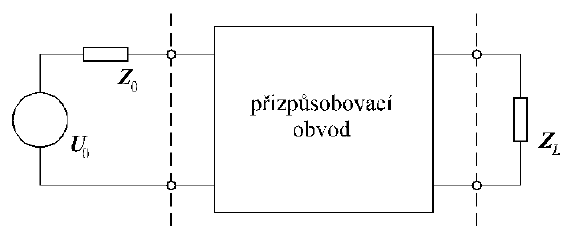
\includegraphics[width=0.5\linewidth]{RA_smith01.png}
          \caption{Umístění přizpůsobovacího obvodu mezi zátěží a zdrojem signálu (vedením)}
          \label{fyz:fig_RA_smith01} 
        \end{figure}
        K tomuto účelu vystačíme s nejjednodušším typem zapojení, které umožňuje dosažení 
        přizpůsobení na jednom kmitočtu s tzv. \(\Gamma\text{-články}\). Jde o kaskádní řazení 
        dvojice reaktančních prvků, z nichž jeden je vždy v podélné a druhý v příčné větvi bez 
        ohledu na pořadí. V rezistivních obvodech totiž dochází ke ztrátám přenášeného výkonu, 
        zatímco obvody složené z reaktancí slibují (alespoň teoreticky) dosažení přizpůsobení beze 
        ztrát. Kombinací obou pořadí s typy reaktančních prvků (kondenzátor, cívka) dostáváme 
        celkem osm různých možností uspořádání \(\Gamma\text{-článků}\), přičemž volba konkrétní 
        struktury závisí především na hodnotě přizpůsobované impedance \(Z_L\). Obrázek 
        \ref{RA:fig_smith02}  ukazuje jednotlivé vhodné struktury v závislosti na umístění 
        impedance \(Z_L\) v impedančním Smithově diagramu v jedné z osmi oblastí \emph{A} až 
        \emph{H}, při aplikaci požadavku přesunu z bodu \(Z_L\) do bodu \(Z_0\) co nejkratší 
        cestou. Hlavní myšlenka zde spočívá v tom, že do bodu \(Z_0\) se lze dostat jedině pohybem 
        po kružnici jednotkové reálné části impedance (\(r = 1\)) nebo admitance (\(y = 1\)), a to 
        buď po směru nebo proti směru hodinových ručiček. To zajišťuje první prvek 
        \(\Gamma\text{-článku}\) – sériově nebo paralelně řazený induktor nebo kapacitor. Z toho 
        plynou čtyři varianty označené malými písmeny „\emph{a}“ až „\emph{d}“. Úkolem 
        druhého stupně je přesun z bodu \(Z_L\) na jednu (obvykle tu nejbližší) z obou zmíněných 
        kružnic opět sériově nebo paralelně řazeným induktorem nebo kapacitorem – odtud tedy osm 
        variant přizpůsobení v oblastech \emph{A} až \emph{D}. Způsob návrhu 
        \(\Gamma\text{-článku}\) pomocí Smithova diagramu nejlépe objasníme na číselném příkladu.
  
        \begin{figure}[ht!] %\ref{RA:fig_smith02} 
          \centering
          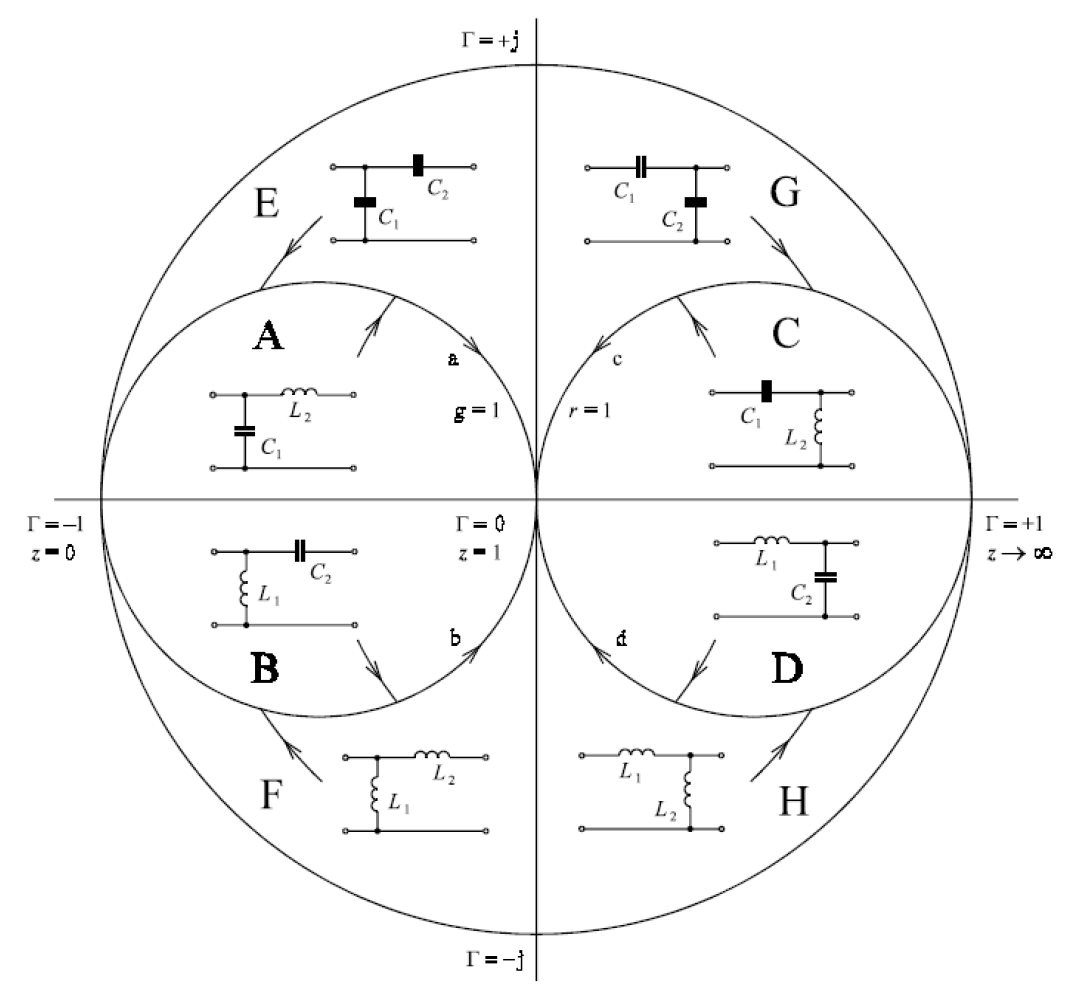
\includegraphics[width=\linewidth]{RA_smith02.png}
          \caption{Vhodné způsoby přesunu ve Smithově diagramu a odpovídající struktury  
          \(\Gamma\text{-článků}\)}
          \label{RA:fig_smith02} 
        \end{figure}
        %------------------------------------
          % !TeX spellcheck = cs_CZ
% RA_exam01.tex
\begin{example}
  Navrhněte graficko-početní metodou ve Smithově diagramu přizpůsobovací obvod pro 
  \(Z_L = \qty{30 - 65j}{\ohm}\) , \(Z_S = 50\)  a \(f = \qty{100}{\MHz}\).
  
  \textbf{Řešení:}
  Platí \(z_L = \dfrac{Z_L}{Z_S} = \num{0.6000 - 1.3000i}\), daný bod se tedy nachází ve 
  \textbf{4. kvadrantu}, \textbf{vně} kružnice konstantní reálné části impedance \(r = 
  1\). Proto volíme strukturu typu \(H\) viz. obr. \ref{RA:fig_smith02}. 
  \newline
  \begin{itemize}
    \item 1. krok: Začínáme v admitančních souřadnicích. Pro posun z bodu \(y_L = 
          \dfrac{1}{z_L} = \num{0.2927 + 0.6341i}\) nejkratší cestou na kružnici \(r = 1\), 
          tj. do bodu \(y_1 = \num{0.2927 + 0.4500i}\), musíme z admitance \(y_L\) ubrat 
          normovanou susceptanci \(\num{0.6341} - \num{0.4500} = \num{0.1841} = \Delta b = 
          \dfrac{\omega L_2}{Z_0}\). Paralelní indukčnost \(L_2\) tedy bude
          \MULTIPLY{2}{\numberPI}{\nmbrA}
          \MULTIPLY{\nmbrA}{100}{\nmbrB}
          \MULTIPLY{\nmbrB}{0.1841}{\nmbrC}
          \DIVIDE{50}{\nmbrC}{\nmbrD}
          \MULTIPLY{1000}{\nmbrD}{\nmbrE}
          \ROUND[2]{\nmbrE}{\sol}
          \begin{equation*}
            L_2 = \frac{Z_0}{\omega\abs{\Delta b}} = 
                  \frac{50}{2\cdot\pi\cdot\num{100e6}\cdot\num{0.1841}} = \qty{\sol}{\nano\henry}
          \end{equation*}
    
           {\centering   %\ref{RA:fig_RA_ADS_smith01} 
            \captionsetup{type=figure}
            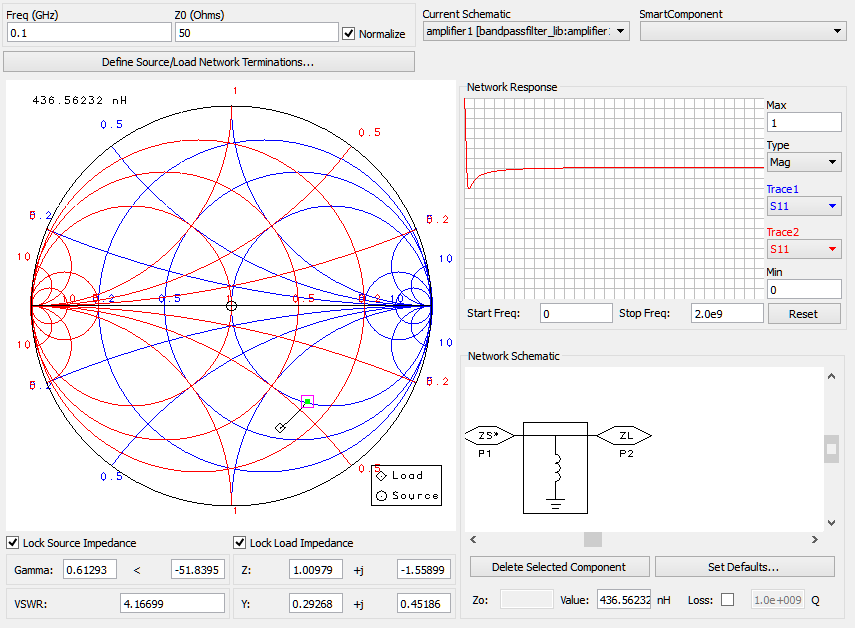
\includegraphics[width=0.8\linewidth]{ADS_smith01.png}
            \captionof{figure}{ADS Smith Chart tool: Přechod z bodu \(y_L \rightarrow y_1\)}
            \label{RA:fig_ADS_smith01} 
            \par}
          
    \item 2.krok: Pro posun z bodu \(z_1 = \dfrac{1}{y_1} = \num{1 - 1.5479i}\) do bodu 
          \(z_S = \num{1 + 0i}\) musíme k \(z_1\) přidat normovanou reaktanci \(1.5479 = \Delta 
          x = \frac{\omega L_2}{Z_0}\). Sériová indukčnost \(L_1\) tedy bude
          \MULTIPLY{2}{\numberPI}{\nmbrA}
          \MULTIPLY{\nmbrA}{100}{\nmbrB}
          \MULTIPLY{50}{1.5479}{\nmbrC}
          \DIVIDE{\nmbrC}{\nmbrB}{\nmbrD}
          \MULTIPLY{1000}{\nmbrD}{\nmbrE}
          \ROUND[2]{\nmbrE}{\sol}
          \begin{equation*}
            L_1 = \frac{\Delta x Z_0}{\omega} = 
                  \frac{\num{1.5479}\cdot\num{50}}{2\cdot\pi\cdot\num{100e6}} = 
                  \qty{\sol}{\nano\henry}
          \end{equation*}
           
           {\centering   %\ref{RA:fig_RA_ADS_smith02}
            \captionsetup{type=figure} 
            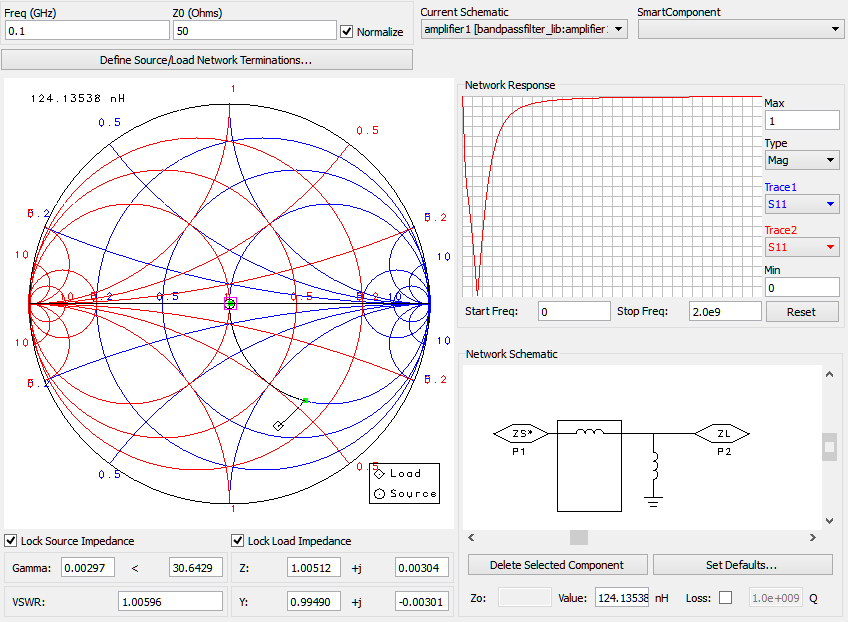
\includegraphics[width=0.8\linewidth]{ADS_smith02.png}
            \captionof{figure}{ADS Smith Chart tool: Přechod z bodu \(z_1 \rightarrow z_S\)}
            \label{RA:fig_ADS_smith02} 
            \par} 
  \end{itemize}
\end{example} 
        %------------------------------------
        Kromě přesunu nejkratší cestou přicházejí v úvahu ještě další varianty spojené s přechodem 
        do jiného segmentu. Např. pro \(Z_L\) v oblasti \(A\) lze použít též 
        \(\Gamma\text{-článek}\) typu \(B\); pro \(Z_L\) v oblasti \(E\) lze použít též typy \(B\), 
        \(D\) nebo \(G\) apod. Pro dosažení nejmenší kmitočtové závislosti lze však obvykle 
        doporučit pouze přesun nejkratší cestou.
  
      \subsubsection{Smithův diagram}
        \emph{Impedanční Smithův diagram} je soustava křivek (přesněji kružnic nebo jejich částí) 
        tvořených body normované impedance \(z\) s konstantní reálnou či imaginární částí 
        zakreslených v komplexní rovině činitele odrazu \(\Gamma\) definovaná konformním zobrazením
        \begin{equation}\label{RA:eq_smith07}
          \Gamma = \frac{z-1}{z+1}.
        \end{equation} 
  
        Každému bodu v Smithově diagramu odpovídá jedna hodnota normované impedance \(z = r + jx\), 
        a odnormované impedance \(Z = R+jX\). Otočením o 180°, popř. středovou souměrností, 
        získáme \emph{admitanční Smithův diagram} \(y = g + jb\), resp. \(Y = G + jB\). Kružnice 
        konstantních reálných částí se sbíhají v bodě \(1\) a mají středy na reálné ose. Kružnice 
        (části kružnic) konstantní imaginární části se taktéž sbíhají v bodě \(1\) a mají středy na 
        přímce Re [] = 1.
  
        Jelikož pro převod mezi poměrem stojatých vln a modulem činitele odrazu j􀀀j platí stejný 
        vztah jako mezi činitelem odrazu 􀀀 a normovanou impednací z, tj.
        \begin{equation}\label{RA:eq_smith08}
          \Gamma = \frac{z-1}{z+1} \qquad \Leftrightarrow 
          \abs{\Gamma} = \frac{\abs{PSV}-1}{z+\abs{PSV}}.
        \end{equation} 
        s rozdílem, že PSV je vždy reálné číslo větší nebo rovno jedné, lze PSV pro daný bod ve 
        Smithově diagramu určit z průsečíku kružnice se středem v bodě z = 0 a poloměrem j􀀀j a 
        části reálné osy normované impedance mezi body z = 1 a z ! 1.
        
      \subsubsection{Měření činitěle odrazu} 
        Abychom mohli měřit činitel odrazu podle definice (1), musíme mít možnost
        \begin{itemize}
          \item oddělit vlnu odraženou (U¡) od vlny dopadající (U+)
          \item měřit komplexní poměr fázorů napětí na příslušném kmitočtu.
        \end{itemize} 
        
        Splnění prvního požadavku nám zajišťuje tzv. směrový vazební člen (SVČ), splnění druhého 
        požadavku pak vektorový voltmetr. Celkové uspořádání měřicí sestavy využívající směrového 
        vazebního členu a vektorového voltmetru znázorňuje obr. 3. Harmonický signál potřebného 
        kmitočtu se rozděluje pomocí symetrického přizpůsobeného T-článku (splitteru) do tzv. 
        referenční a měřicí větve. Obě větve jsou zakončeny terminátory o impedanci rovné vlnové 
        impedanci Z0 vedení a konektorů, aby zde nedocházelo k nežádoucím odrazům a stojatému 
        vlnění. Ke snížení stojatého vlnění též přispívají pevné útlumové články v obou větvích 
        (20, 14 a 6 dB). Napětí v obou větvích jsou snímána sondami vektorového voltmetru 
        zasunutými do průchozích držáků. Měřená zátěž ZL je připojena na konec hlavního vedení 
        směrového vazebního členu SVč . Odražená vlna se potom vyvazuje na bránu 4 (přes vazbu K2 
        SVČ) a její amplituda a fáze je měřena sondou B vektorového voltmetru. Sonda A v referenční 
        větvi poskytuje fázovou referenci pro stanovení fáze činitele odrazu.
  
        Měření činitele odrazu probíhá ve dvou krocích:
        \begin{itemize}
          \item Nastavení amplitudové a fázové referenční hodnoty. Měřicí aparaturu je třeba 
          zkalibrovat tak, aby udávaný modul a fáze činitele odrazu pro nějakou zátěž, jejíž 
          činitel odrazu předem známe, této hodnotě přesně odpovídal. K tomuto účelu se obvykle 
          používá zkrat (Z = 0, 􀀀 = ¡1;0), ale v našem konkrétním případě se jako vhodnější ukazuje 
          otevřený konec vedení (Z ! 1, 􀀀 = +1;0), neboť naměřená odražená vlna při něm vykazuje o 
          něco větší amplitudu než při zakončení zkratem. Bránu 3 SVč (konec hlavního vedení) tedy 
          necháme nezakončenou a na generátoru nastavíme příslušný kmitočet f a vhodnou amplitudu 
          (zpravidla největší přípustnou, pro dobrý odstup signálu od šumu ve vektorovém 
          voltmetru). Amplitudu napětí naměřenou v této situaci sondou B uložíme na přístroji 
          BM553 jako referenční stlačením tlačítek <B>, <LEVEL REF STORE> a fázový rozdíl 'B ¡'A 
          uložíme jako referenční tlačítkem <',T REF STORE>. Aplikaci uložené amplitudové 
          referenční hodnoty poté aktivujeme tlačítkem <LIN REF>. Přístroj by měl zobrazovat 
          správnou hodnotu 􀀀 pro zakončení naprázdno, tj. modul 1;0 a fázi 0±.
  
          \item Vlastní měření činitele odrazu 􀀀. Na bránu 3 směrového vazebního členu připojíme 
          měřenou zátěž. Bylo-li provedeno nastavení podle předchozího bodu, bude již přístroj 
          ukazovat správnou hodnotu činitele odrazu 􀀀 v polárních souřadnicích.   
        \end{itemize}
        
        Z uspořádání měřicího systému je zřejmé, že při měření činitele odrazu na více kmitočtech 
        je třeba po každé změně kmitočtu signálu celý první krok postupu zopakovat.
  
      \subsubsection{Směrový vazební člen}     
        Směrový vazební člen (SVČ, též směrová vazební odbočka, směrová vazební odbočnice, směrová 
        vazba) je vysokofrekvenční čtyřbran umožňující oddělení a měření složek signálu, které se 
        šíří po vedení pouze jedním směrem. Mezi jeho četné aplikace patří měření činitele odrazu, 
        oddělení signálního generátoru od měřicích obvodů, rozdělení výkonu a připojení dalších 
        přístrojů (vlnoměrů, analyzátorů, wattmetrů apod.).
  
        Princip SVČ je založen na vlastnostech obvodů s rozprostřenými parametry a jeho vnější 
        funkce je patrná z obrázku 4. Dva úseky vedení ‚- hlavní (zakončené branami 1 a 3) a 
        vedlejší/vazební (mezi branami 2 a 4) ‚- jsou spojeny tak, aby mezi nimi vznikla vazba. 
        Tato vazba způsobuje, že se signál zavedený na bránu 1 hlavního vedení rozdělí v určitém 
        poměru na dvě vzájemně fázově posunuté složky. Jedna složka vystupuje na bráně 3 a druhá 
        bud’ na bráně 2, přičemž brána 4 je dokonale izolována (protisměrný SVČ ), nebo na bráně 4, 
        přičemž brána 2 je izolována (souměrný SVČ ). Zmíněná vazba je reciprocitní a vykazuje 
        obdobné chování i ze směru od vedlejšího vedení k hlavnímu.      
  
        \begin{figure}\ref{fyz:fig_RA_smith03} 
          \centering
          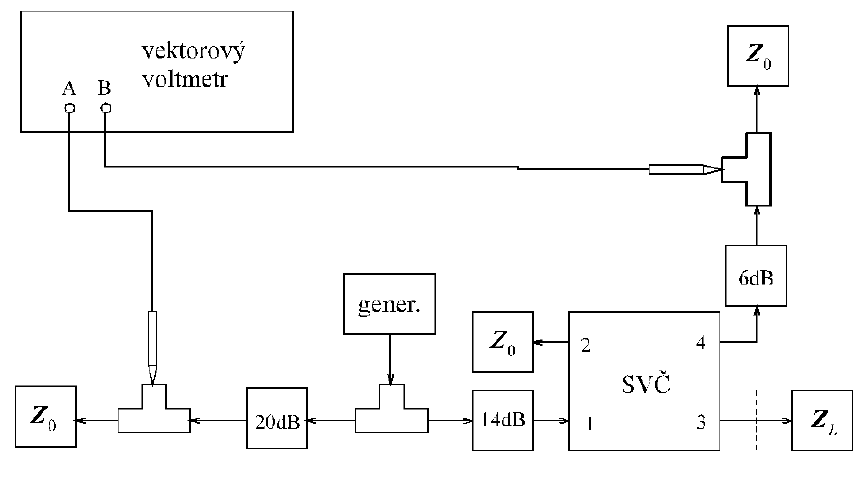
\includegraphics[width=\linewidth]{RA_smith03.png}
          \caption{Směrový vazební člen jako čtyřbran}
          \label{fyz:fig_RA_smith03} 
        \end{figure}
  
        SVČ lze popsat maticí rozptylových parametrů o rozměru 4 Q 4, kde parametry skk na hlavní 
        diagonále jsou činitele odrazu na jednotlivých branách, ostatní parametry jsou činitele 
        přenosu mezi branami. U ideálního protisměrného (obr. 4) SVč jsou všechny činitele odrazu 
        rovny nule, přenos z brány 1 na bránu 4 je též nulový a s ohledem na symetrii SVč jsou 
        nulové i přenosy mezi branami 4–1, 2–3 a 3–2. Rozptylová matice ideálního SVč potom tedy je
  
        \begin{equation}\label{RA:eq_smith09}
          s = \left[
            \begin{matrix}
                0    & s_{12} & s_{13} &  0       \\
              s_{21} &   0    &   0    & s_{24}   \\
              s_{31} &   0    &   0    & s_{34}   \\
                0    & s_{42} & s_{43} &  0     
            \end{matrix}
              \right]
        \end{equation} 
  
        Vzhledem k aplikaci SVč a symetrii matice s-parametrů se SVč často charakterizují několika 
        skalárními parametry vycházejícími z s-parametrů resp. výkonové bilance na branách SVč . 
        Jsou to tyto parametry: vazba K (K1, K2, též tzv. přeslechový útlum), směrovost D, izolace 
        I a taktéž kmitočtový rozsah.
  
        Vazba K (též K1) je definována jako poměr výkonu P1 přiváděného na vstup hlavního vedení 1 
        a výkonu P2 vystupujícího z brány 2 při bezodrazovém zakončení bran 2 až 4,
        \begin{equation}\label{RA:eq_smith10}
          K = K_1 = 10\log\frac{P_1}{P_2} 
                  = 10\log\frac{1}{\abs{s_{21}}^2} = -20\log\abs{s_{21}},  
        \end{equation} 
        a vyjadřuje tedy vazební útlum přímé vlny na hlavním vedení (směřující od brány 1 k bráně 
        3) na vstup vedlejšího vedení 2.
  
        Podobně vazba K2 je definována jako poměr výkonu P3 přiváděného na výstup hlavního vedení 3 
        a výkonu P4 vystupujícího z brány 4 při bezodrazovém zakončení bran 1, 2 a 4,
        \begin{equation}\label{RA:eq_smith11}
          K_2 = 10\log\frac{P_3}{P_4} 
              = 10\log\frac{1}{\abs{s_{43}}^2} = -20\log\abs{s_{43}},  
        \end{equation} 
        a vyjadřuje tedy vazební útlum zpětné vlny na hlavním vedení (směřující od brány 3 k bráně 
        1) na výstup vedlejšího vedení 4.
  
        Směrovost D je definována jako poměr výkonu P2 vystupujícího z brány 2 a výkonu P4 
        vystupujícího z brány 4 při přivádění signálu na bránu 1 a bezodrazovém zakončení bran 2 až 
        4,
        \begin{equation}\label{RA:eq_smith12}
          D = 10\log\frac{P_2}{P_4} 
            = 10\log\frac{1}{\abs{s_{42}}^2} = -20\log\abs{s_{42}},  
        \end{equation} 
  
        Izolace I je definována jako poměr výkonu P1 přiváděného na vstup hlavního vedení 1 a 
        výkonu P4 vystupujícího z brány 4 při bezodrazovém zakončení bran 2 až 4,
        \begin{equation}\label{RA:eq_smith13}
          I = 10\log\frac{P_1}{P_4} 
            = 10\log\frac{1}{\abs{s_{41}}^2} = -20\log\abs{s_{41}}, 
        \end{equation} 
        a vyjadřuje tedy vazební přeslechový útlum mezi přímou vlnou na hlavním vedení (směřující 
        od brány 1 k bráně 3) a výstupem vedlejšího vedení 4.
  
        Z uvedených definic plyne, že směrovost D je rovna rozdílu izolace I a vazby K (resp. K1)
        \begin{equation}\label{RA:eq_smith14}
          D = I - K = I - K_1 = 20\log\frac{\abs{s_{21}}}{\abs{s_{41}}}
        \end{equation}  
  
        Směrovost D (v souladu se svým názvem) popisuje schopnost směrové selekce – čím je větší, 
        tím méně se při měření vlny signálu v jednom směru pomocí SVč nežádoucím způsobem projevuje 
        vlna šířící se v opačném směru.
  
      \subsection{Vektorový voltmetr}
        Vektorový voltmetr je schopen měřit amplitudy dvou harmonických signálů \(U_A\) a \(U_B\) a 
        jejich fázový rozdíl \(\varphi_B - \varphi_A\). Dále bývá obvykle schopen měřit poměr 
        amplitud \(\frac{U_B}{U_A}\) a také umožňuje i relativní měření vůči uložené a různá 
        odvozená měření (např. s-parametrů, R, L, C prvků apod.) využívající zvláštní příslušenství.
  
        Princip vektorového voltmetru je založen na vzorkování obou měřených signálů a jejich 
        současném převodu na nízký mezifrekvenční kmitočet 20 kHz. Takto nízký kmitočet lze již 
        snadno a přesně zpracovat, jednak detektory a A/D převodníky pro zjištění amplitudy, jednak 
        logickými obvody pro zjištění fázového rozdílu. Vzorkování se provádí velmi rychlými 
        analogovými spínači se Schottkyho diodami umístěnými přímo v sondách. Vzorkovací kmitočet 
        se musí od kmitočtu měřeného signálu lišit přesně o 20 kHz, což je zajištěno pomocí smyčky 
        automatické kmitočtové a fázové synchronizace uvnitř voltmetru.  

%---------------------------------------------------------------------------------------------------
\printbibliography[heading=subbibliography]
\addcontentsline{toc}{section}{Seznam literatury}  % ** TODO
%================================= Kapitola: Přehled jazyka C++=====================================
%  %============= Kapitola: Simthův diagram v radiotechnice  ==========================================
\setchaptertoc
\chapter{Simthův diagram v radiotechnice}\label{chap:ra_smith}


    \begin{figure}[ht!]  % \ref{fig_RA:modulace04}
      \centering
      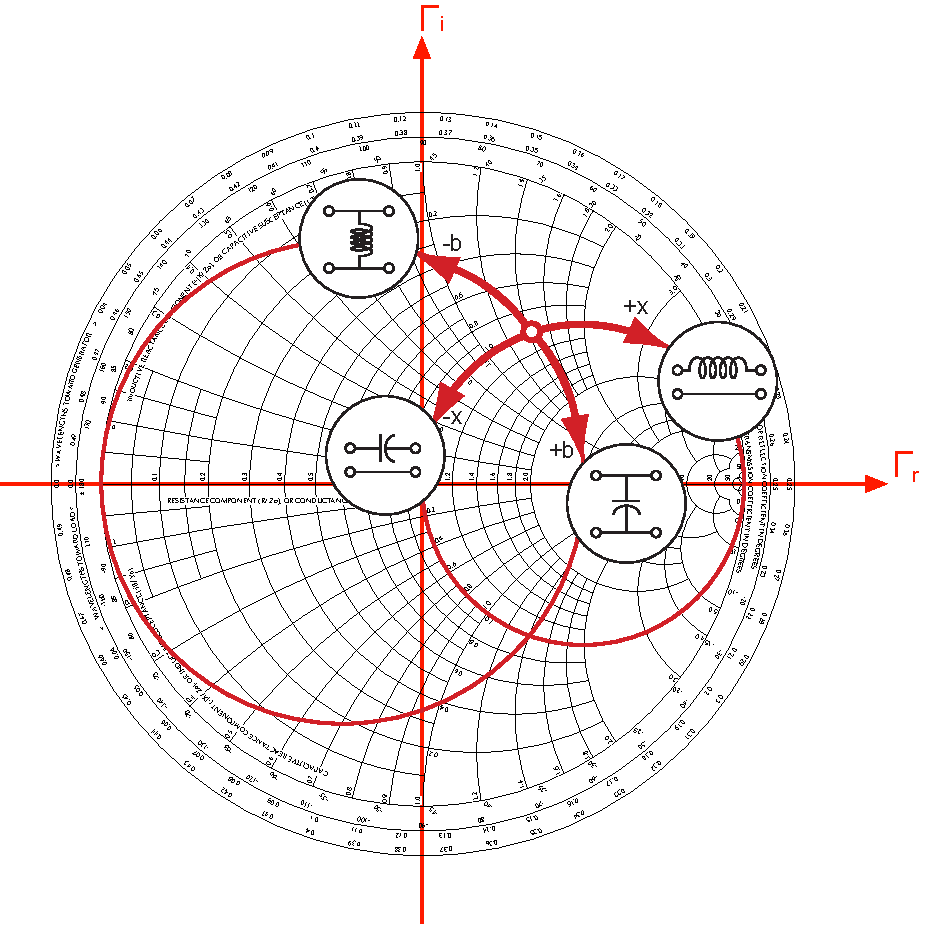
\includegraphics[width=1\linewidth]{smith_chart01.pdf}
      \caption{Smith Chart: Effect of Adding Series Reactances or Shunt Susceptances 
               \cite[s.~45]{IEEEStearns2001}}
      \label{fig_RA:smith01}
    \end{figure}
    
%--------------------------------------------------------------------------------------------------- % ** TODO
%================================= Kapitola: Přehled jazyka C++=====================================
  % !TeX spellcheck = cs_CZ
%=============== Kapitola: Antény: Teoretický základ ===============================================
\chapter{Antény: Teoretický základ}\label{chap:ra_antennatheory}
\minitoc

  \section{Teoretický základ}
    Když jsme se na počátku našeho výkladu zabývali šířením vln, nezajímali jsme se o to, jak vlny 
    vznikly. Proces vzniku vlnění v prostoru (proces vyzařování) bude vyšetřováno v této kapitole. 
    
    Z fyziky je známo, že zdrojem elektromagnetických vln je střídavý (vysokofrekvenční) proud. 
    Úlohu o vyzařování můžeme tedy formulovat tak, že známe proud tekoucí v prostoru (na vysílací 
    anténě) a chceme zjistit, jaké intenzity polí vytvoří tento proud kdekoli jinde v prostoru. 
    Matematicky jde o \textbf{řešení nehomogenní soustavy Maxwellových rovnic:}
    \begin{align}\label{RA:eq_ant01}
      \rot{H} &= \vec{J} + j\omega\varepsilon\vec{H} \\
      \rot{E} &= -j\omega\mu\vec{H}
    \end{align}
    v níž proudová hustota \(\vec{J}\) je známá a intenzity \(\vec{E}\) a \(\vec{H}\) se hledají 
    \cite[s.~33]{Hanus2002}. 
    
    \subsection{Impedance lineárních antén}
      Lineární anténa je \emph{jednobran} a poměr fázorů vstupního napětí a vstupního proudu 
      definuje  tzv. \textbf{vstupní impedanci antény}. Vstupní impedance je veličina stejně 
      důležitá jako funkce záření, protože rozhoduje o přizpůsobení antény k napájecímu vedení. 
      Vstupní impedance je obecně komplexní: má reálnou část (\emph{vstupní odpor}) a imaginární 
      část (\emph{vstupní reaktanci}). Obě složky bezprostředně souvisí s činností antény. Anténa 
      vyzařuje jistý činný výkon, a tudíž nejméně stejný činný výkon musí také odebírat ze zdroje. 
      Z hlediska uživatele se musí jevit na svorkách antény takový reálný odpor, který by odebíral 
      tentýž výkon. Ve skutečnosti má anténa ztráty (část přivedeného činného výkonu se mění v 
      teplo), takže odebíraný výkon bude o něco větší a odpor na svorkách také. Kromě toho anténa 
      během každé periody si vyměňuje energii s elektromagnetickým polem ve svém blízkém 
      okolí a to se projeví existencí jisté reaktance na vstupu. Této úvaze odpovídá náhradní obvod 
      antény nakreslený na obr. \ref{RA:fig_001} \cite[s.~44]{Hanus2002}.

      \begin{figure}[ht!]   %\ref{RA:fig_001}
        \centering
        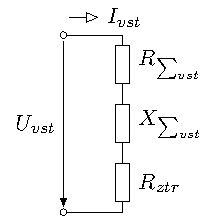
\includegraphics[width=0.5\linewidth]{RA001.pdf}
        \caption{Náhradní obvod antény}
        \label{RA:fig_001}
      \end{figure}
      
      Odpor \(R_{\sum_{vst}}\) je tzv. \textbf{odpor záření antény} vztažený ke vstupnímu proudu. 
      Místo odpor záření se užívají také názvy \emph{vyzařovací odpor} nebo \emph{zářivý odpor}. 
      Odpor  \(R_{ztr}\) je \textbf{ztrátový odpor antény}. V součinu se čtvercem efektivní hodnoty 
      vstupního proudu tyto odpory určují \textbf{vyzařovaný a ztrátový výkon antény}:
      \begin{itemize}\addtolength{\itemsep}{-0.5\baselineskip}
        \item \emph{vyzařovaný výkon:} \(P_{\sum} = I^2_{vst_{ef}}\cdot R_{\sum_{vst}}\)
        \item \emph{ztrátový výkon:}   \(P_{ztr} = I^2_{ztr_{ef}}\cdot R_{ztr}\)
      \end{itemize}
      Protože na anténě je obvykle stojaté vlnění, je proud v každém místě jiný. Vyzařovaný výkon 
      je však jeden. Podle prvního z uvedených vztahů přísluší tedy každému proudu, a tedy i 
      každému místu na anténě, jiná hodnota odporu záření. Nebo naopak, každá hodnota odporu záření 
      je \emph{vztažena} k určitému proudu (místu) na anténě. Nejčastěji se odpor záření vztahuje 
      buď k proudu vstupnímu (\(I_{vst}\)) nebo k proudu v kmitně (\(I_{max}\)). Vyzařovaný výkon 
      je tedy alternativně
      \begin{equation}\label{RA:eq_ant02}
        P_{\sum} = I^2_{vst_{ef}}\cdot R_{\sum_{vst}} = I^2_{max_{ef}}\cdot R_{\sum_{m}}
      \end{equation} 
      \(R_{\sum_{m}}\) je \emph{odpor záření vztažený ke kmitně proudu}. Vztah (\ref{RA:eq_ant02}) 
      umožňuje přepočítat odpor záření z jednoho místa do druhého, známe-li funkci \emph{proudové 
      distribuce}. 
      
      
     
  \section{Parametry antén}
    Elektrické vlastnosti antén různých typů se charakterizují stručnými číselnými údaji, které 
    nazýváme parametry. Jejich znalost je důležitá při navrhování rádiových soustav 
    \cite[s.~46]{Hanus2002}. 

     % In many situations, a good match is defined arbitrarily as having SWR<1.5. 
     V mnoha aplikacích se dosažené impedanční přizpůsobení považuje dobré je-li \(\text{VSWR}<1,5\)
     \begin{align}
       \text{VSWR} &= \frac{1+\abs{\Gamma}}{1-\abs{\Gamma}} \qquad \Rightarrow \qquad
                     \abs{\Gamma} = \frac{\text{VSWR}-1}{\text{SWR}+1}, \\
       \shortintertext{a odražený výkon lze jednoduše získat jako mocninu amplitudy koeficientu 
         odrazu} 
       R_L &= -10\log\abs{\Gamma}^2 = -20\log\abs{\Gamma} \qquad\si{\decibel} \\
       \shortintertext{and the transmitted power to the load, relative to the incident wave power, 
         is}
       T_L &= -10\log(1 - \abs{\Gamma}^2) \qquad\si{\decibel}
     \end{align}
     
     
    \begin{table}[ht!]
      \centering
      \begin{tabular}{c|ccc}
        \rowcolor[HTML]{000000} 
        \multicolumn{1}{c}{\cellcolor[HTML]{000000}
          {\color[HTML]{FFFFFF} \textbf{VSWR}}}      & 
          {\color[HTML]{FFFFFF} \textbf{\(\abs{\Gamma}\)}} & 
        \multicolumn{2}{c}{\cellcolor[HTML]{000000}
          {\color[HTML]{FFFFFF} \textbf{Odražený výkon}}}          \\ 
        \rowcolor[HTML]{000000}{\color[HTML]{FFFFFF} }           &
                               {\color[HTML]{FFFFFF} \(\abs{s_{11}}\)}  & 
                               {\color[HTML]{FFFFFF} (\%)}       & 
                               {\color[HTML]{FFFFFF} (dB)}           \\
         1.0 & 0.000 &  0.0 & \(\infty\)  \\
         1.5 & 0.200 &  4.0 & 14.0  \\
         2.0 & 0.333 & 11.1 & 9.55  \\
         2.5 & 0.429 & 18.4 & 7.36  \\
         3.0 & 0.500 & 25.0 & 6.00  \\
         3.5 & 0.556 & 30.9 & 5.10  \\
         4.0 & 0.600 & 36.0 & 4.44  \\
         5.0 & 0.667 & 44.0 & 3.52  \\
         6.0 & 0.714 & 51.0 & 2.92  \\
         7.0 & 0.750 & 56.3 & 2.50  \\
         8.0 & 0.778 & 60.5 & 2.18  \\
         9.0 & 0.800 & 64.0 & 1.94  \\
        10.0 & 0.818 & 66.9 & 1.74  \\
        15.0 & 0.875 & 76.6 & 1.16  \\
        20.0 & 0.905 & 81.9 & 0.87  \\
        50.0 & 0.961 & 92.3 & 0.35  \\ \cline{1-4}
        \hline
      \end{tabular}
      \caption{Demonstrace vzájemného vztahu mezi poměrem stojatých vln \texttt{VSWR}, amplitudy 
               koeficientu odrazu \(\Gamma\) a velikostí odraženého výkonu\protect\footnotemark[1] 
               vyjádřeného v procentech a decibelech. Kredit: \AntTheoVSWR}
      \label{fig_RA:VSWRGammaTable}
    \end{table}

 \footnotetext[1]{Return loss}

%---------------------------------------------------------------------------------------------------
\printbibliography[heading=subbibliography]
\addcontentsline{toc}{section}{Seznam literatury}
%================================= Kapitola: Přehled jazyka C++=====================================
  % !TeX spellcheck = cs_CZ
%============= Kapitola: Modulace===================================================================
\setchaptertoc
\chapter{Modulace}\label{chap:ra_mod}


  %--------------- Rádiové komunikační systémy ----------------==-----------------------------------
  \section{Obecné schéma rádiového komunikačního systému}
    V této kapitole jsou shrnuty základní poznatky o modulacích používaných v rádiové komunikaci. 
    Nejprve se popišme obecné schéma rádiového komunikačního systému podle Shannona, které je na 
    obr. \ref{fig_RA:modulace01}. Toto schéma lze aplikovat především na systémy digitální, tedy 
    například na systémy digitálního rozhlasu a televize, na systémy digitálních celulárních 
    radiotelefonů, na systémy digitálních radiokomunikačních družicových prostředků apod. 
    \begin{figure}[ht!]  % \ref{fig_RA:modulace01}
      \centering
      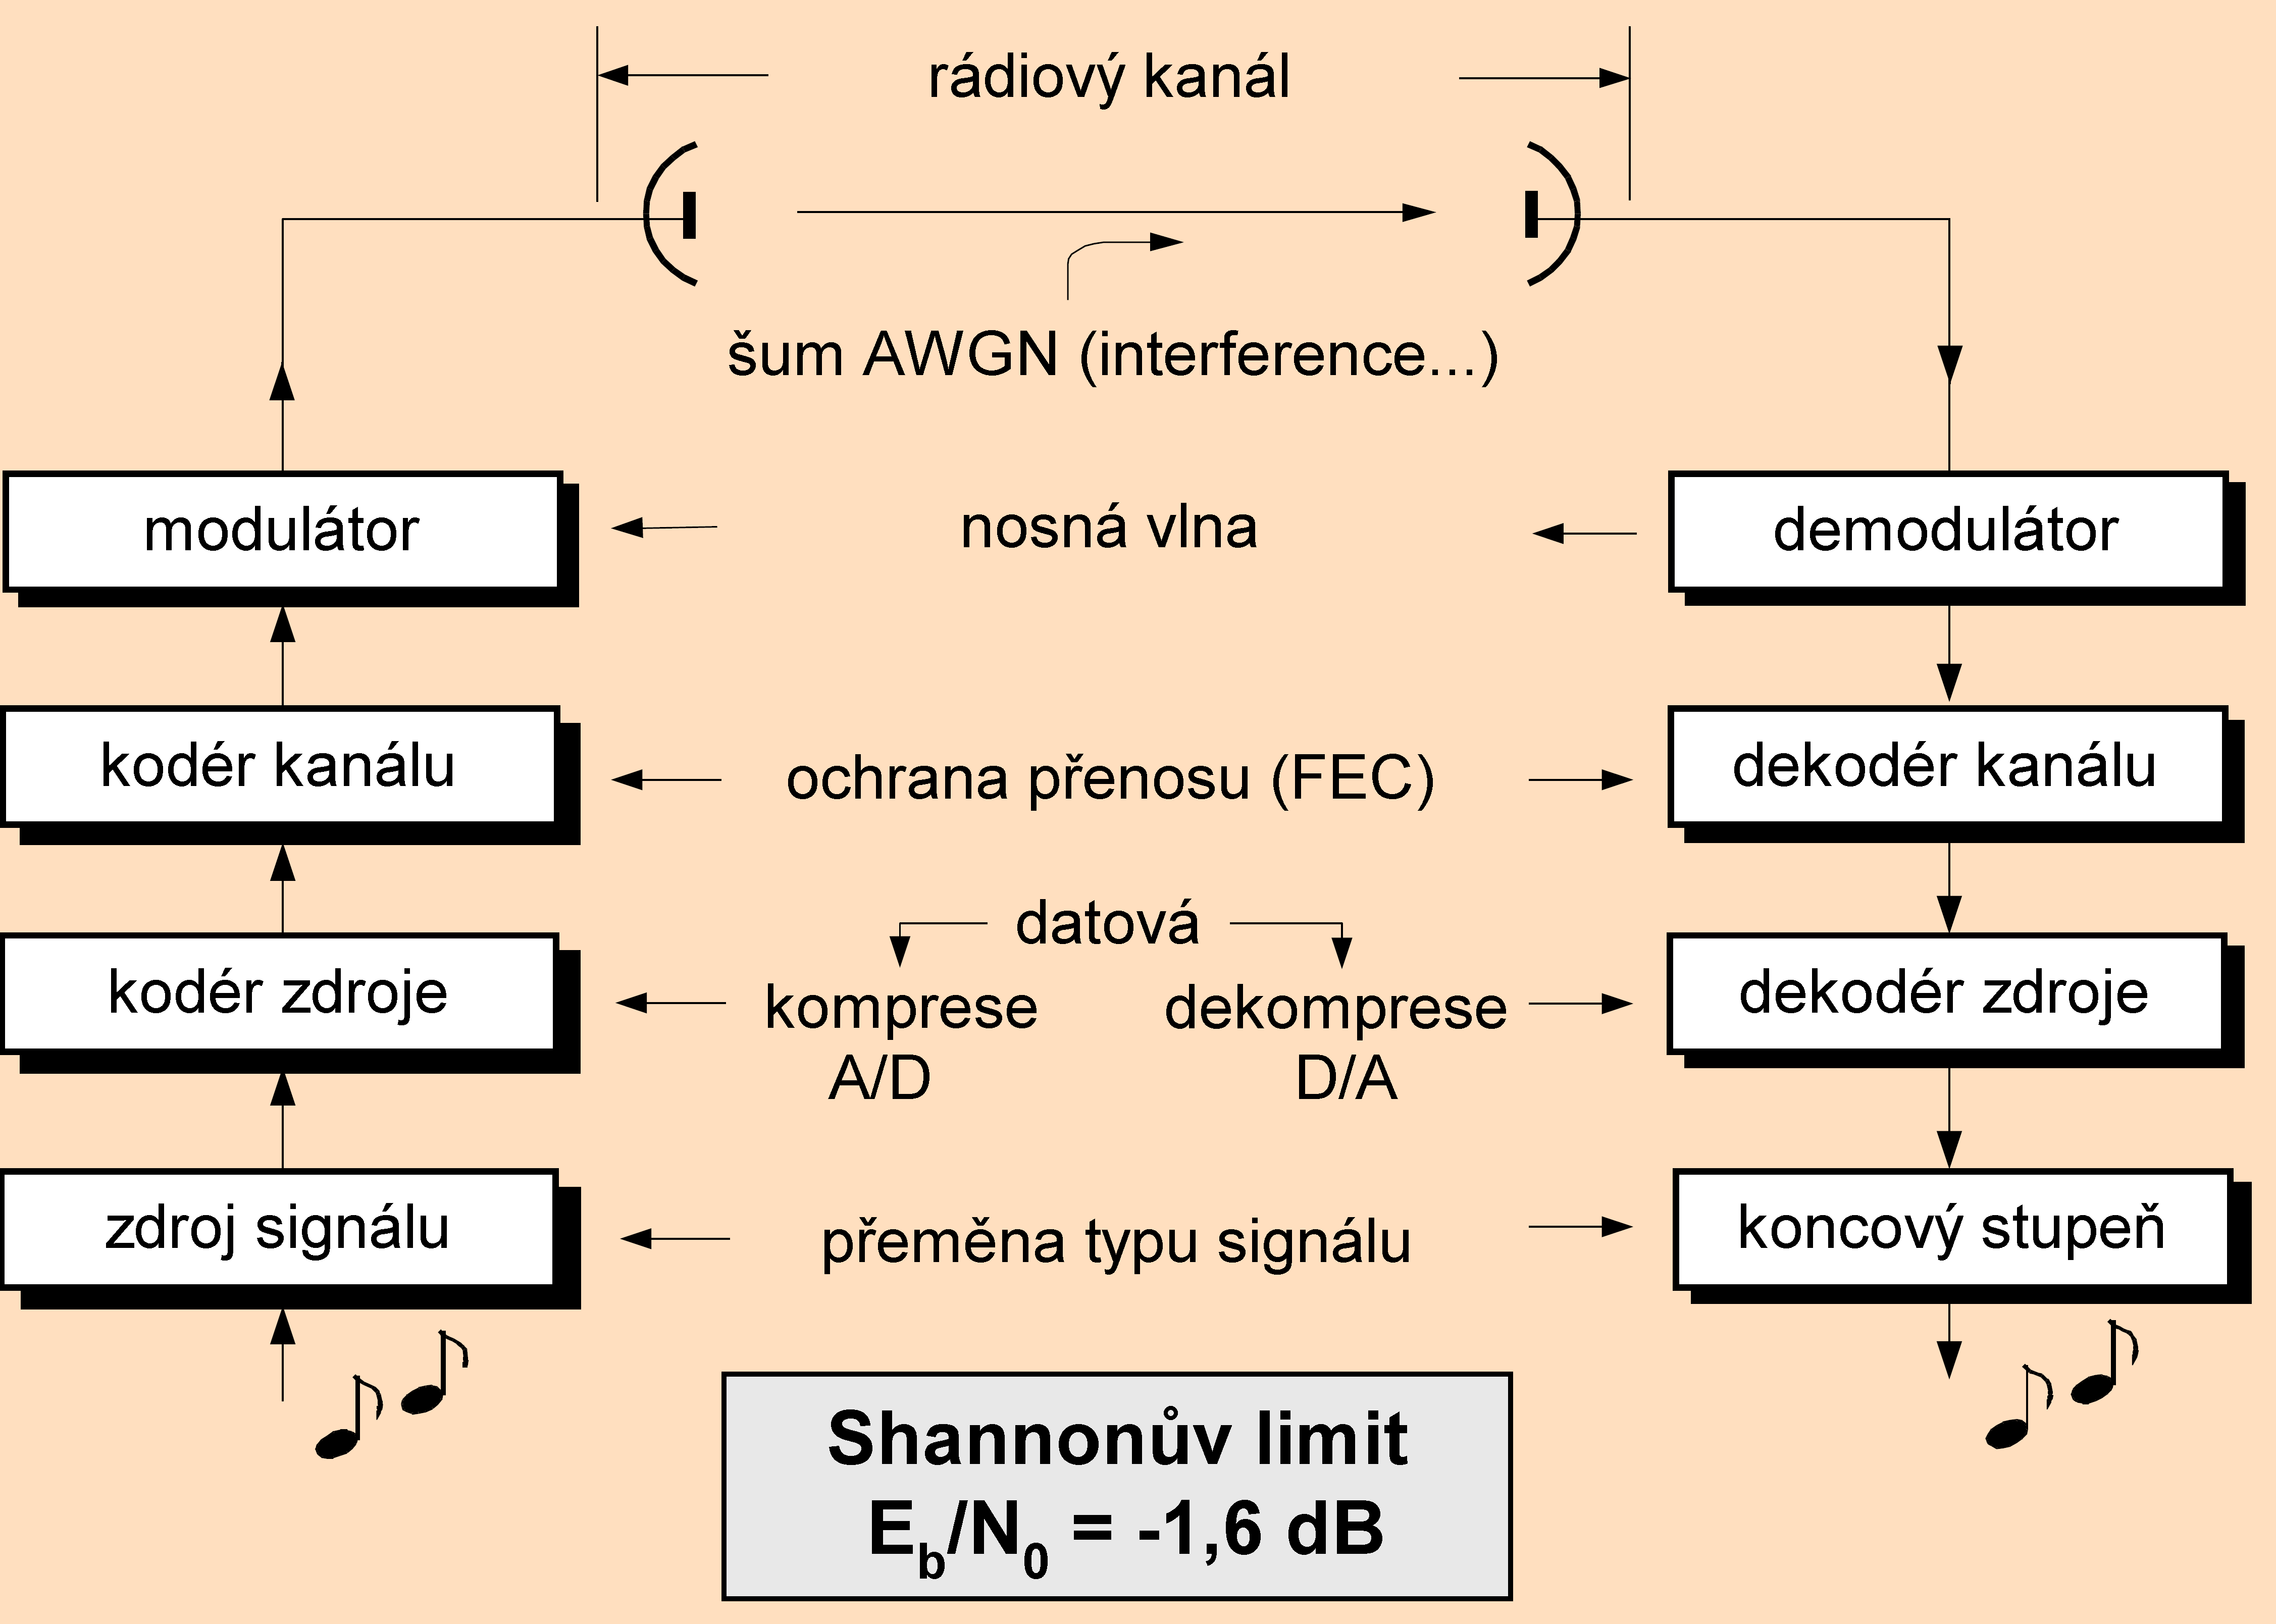
\includegraphics[width=1\linewidth]{shannon_radiokomunikacni_system.png}
      \caption{Obecné Shannonovo schéma radiokomunikačního systému
               \cite[s.~75]{ZaludRA}}
      \label{fig_RA:modulace01}
    \end{figure}
    
    Pokud se však v tomto schématu vypustí některé bloky (kodéry a dekodéry), je použitelné i pro 
    vývojově starší analogové systémy. Přestože toto schéma koncipoval Shannon již v padesátých 
    letech, je dodnes aktuální a po menších úpravách lze pomocí něho modelovat i nejmodernější 
    radiokomunikační zařízení.
    
    Na vstupu vysílače je \textbf{zdroj signálu}, jímž může být např. mikrofon nebo televizní 
    snímací elektronka apod. Ten pře\-mě\-ňu\-je přenášenou informaci, jež může mít v obecném 
    případě původně charakter neelektrické veličiny, na elektrický signál. V následujícím 
    \textbf{kodéru zdroje signálu} se signály přicházející z předchozího bloku nejprve digitalizují 
    (pokud ovšem neměly již předtím digitální podobu) a poté se podrobují vlastnímu zdrojovému 
    kódování. Tím se v nich potlačuje \emph{redundance}, což je nadbytečná informace, která je v 
    akustických, obrazových či jiných informačních tocích pocházejících z „přírodních“ zdrojů 
    většinou velmi výrazně zastoupena; (přesněji bývá redundance definována jako nadbytečnost, 
    resp. větší množství dat, než je nezbytné pro přenos informace vzhledem ke ztrátám v 
    komunikačním kanálu; dokonalá exaktní definice této veličiny je však složitá). Zde se potlačuje 
    také irelevance, volně definovaná jako nepodstatná informace. Účinnost kódování prováděného v 
    kodéru zdroje je tím lepší, čím je rychlost bitového toku na jeho výstupu nižší, než na jeho 
    vstupu; připomeňme, že proces zdrojového kódování se proto také označuje jako proces 
    \emph{komprese dat}, nebo také jako mapování vstupního digitálního signálu zdrojového kodéru na 
    jeho signál výstupní. Toto mapování se uskutečňuje podle určitého jednoznačného algoritmu. 
    Dekodér zdroje signálu na přijímací straně realizující inverzní mapování, již poskytuje na svém 
    výstupu užitečný výstupní signál, který se většinou až na zkreslení, šum a určitou složku 
    neobnovené redundance shoduje se signálem na vstupu kodéru zdroje.
        
    V následujícím \textbf{kodéru kanálu} se k binární užitečné - redundance a irelevance, alespoň 
    částečně zbavené - informační sekvenci naopak určitá \emph{redundantní} složka přidává. Je to 
    však redundance přesně kontrolovaná, která je potom využívána k potlačení rušivého působení 
    šumu a interferencí, způsobujících chybovost přenosu. V nejjednodušších (triviálních) systémech 
    kanálového kódování se prostě každý informační bit přenáší m-krát, kde \(m\) je celé kladné 
    číslo. U složitějších (netriviálních) systémů se informační tok sdružuje do sekvencí po \(k\) 
    bitech, k nimž se potom podle vhodných algoritmů přiřazují („mapují“) určité zakódované 
    sekvence po \(n\) bitech. Objem redundance, která se tímto způsobem přidává k užitečnému 
    signálu, je dán poměrem \(n/k\); reciproká hodnota tohoto poměru \(R_c = k/n\) se potom 
    označuje \emph{rychlost kanálového kódování}, nebo krátce \emph{rychlost}. \emph{Zvýšení 
    rychlosti bitového toku signálu způsobené kanálovým kódováním si bohužel vynucuje i rozšíření 
    potřebné šířky pásma komunikačního kanálu mezi vysílačem a přijímačem}.
    
    Uvedeným dvojím kódováním se získává digitální signál s potlačenou redundancí a irelevancí a se 
    zvýšenou odolností proti faktorům způsobujícím chybovost. Ten dále vchází do 
    \textbf{modulátoru}, kde se moduluje pomocí vhodného digitálního modulačního způsobu (formátu) 
    na vysokofrekvenční, nebo na mikrovlnnou nosnou vlnu. \emph{Modulace} je obecně definována jako 
    \emph{proces, při němž se některý parametr této nosné vlny (amplituda, kmitočet, fáze) mění v 
    rytmu modulačního signálu (definice podle Standardu IEEE)}. Díky využití principů modulace je 
    potom možné přenášet v určitém rádiovém prostředí, na nosných vlnách s různými kmitočty, velké 
    množ\-ství zcela nezávislých modulačních signálů. Některé typy modulací navíc umožňují v 
    procesu demodulace v přijímači zlepšit odstup užitečného signálu od šumu, i když za cenu 
    vyšších nároků na šířku pásma. Kromě toho lze při použití nosných vln o relativně vysokých 
    kmitočtech snáze realizovat vysílací i přijímací antény, účinně převádějící elektrický výstupní 
    výkon vysílačů na elektromagnetické vlny, šířící se potom rádiovým komunikačním kanálem. Zcela 
    obecně lze tedy definovat optimální modulátor jako funkční blok, který co nejlépe přizpůsobuje 
    přenášený modulační signál k parametrům následujícího rádiového komunikačního kanálu. Optimální 
    demodulátor potom naopak přijímaný signál převádí - opět pokud možno co nejvěrněji - na původní 
    modulační signál.
    
    \textbf{Komunikačním kanálem} se obecně rozumí fyzikální pros\-tře\-dí, sloužící k přenosu 
    signálu mezi vysílačem a přijímačem. V případě rádiového kanálu toto pojetí odpovídá schématu 
    na obr. \ref{fig_RA:modulace01}, někdy se však do „kanálu“ zahrnují ještě i výstupní obvody 
    vysílačů a vstupní obvody přijímačů apod., takže v zájmu jednoznačnosti je nezbytné tento 
    termín vždy přesně specifikovat. Kromě zmíněných rádiových kanálů se v praxi uplatňují také 
    vývojově vůbec nejstarší kanály s metalickými spoji používané původně v telegrafii a v 
    telefonii, v novější době potom i kanály s optickými spoji.
    
    \emph{Rádiový komunikační kanál} je specifikován určitými parametry, které mohou mít jednak 
    náhodný a jednak nenáhodný charakter. K užitečnému přenášenému signálu se zde především přidává 
    náhodný šum, o němž se v teoretických úvahách v prvém přiblížení předpokládá, že je to 
    \emph{aditivní bílý Gaussov\-ský šum \texttt{AWGN} (Additive White Gaussian Noise)} připomeňme, 
    že pojem \emph{aditivní} zde značí šum, který se lineárně sčítá s užitečným signálem, aniž by 
    docházelo ke vzájemným intermodulacím; pojem \emph{bílý} označuje šum, jehož výkonová 
    spektrální hustota je konstantní tj. nezávislá na kmitočtu a termín \emph{Gaussovský} potom 
    vyjadřuje skutečnost, že rozložení okamžitých amplitud tohoto šumu se řídí \emph{Gaussovou 
    distribucí}. Do komunikačního kanálu přicházejí dále nejrůznější náhodná \emph{rušení} tj. 
    \emph{interference}, ať již přírodního původu (atmosférické poruchy apod.), nebo pocházející od 
    „průmyslových“ zdrojů (od zapalovacích systémů automobilů, atd.). Mohou se zde však uplatňovat 
    ještě další náhodné jevy jako jsou různé typy \emph{úniků (fadingu)} apod. Kromě těchto 
    parametrů náhodného charakteru zde může být přenos signálu ovlivňován ještě dalšími efekty, 
    které mohou mít za určitých okolností nenáhodný tj. deterministický charakter. Při spojení mezi 
    stacionárním vysílačem a přijímačem takovými nenáhodnými jevy může být \emph{doba šíření 
    signálu kanálem}, jeho \emph{fázový posun} apod. Pokud jsou tyto parametry konstantní, není 
    někdy při studiu daného systému vůbec nutné znát jejich konkrétní hodnoty a dále je neuvažovat.
    
    Jedním ze základních objektivních parametrů pro hodnocení analogových komunikačních systémů je 
    jejich výstupní (po-detekční) \textbf{poměr signál/šum} tj. \(S/N\). Požadovaná hodnota tohoto 
    poměru závisí na konkrétním typu komunikačního systému a na jeho aplikaci; tak například u 
    rozhlasových přijímačů \texttt{VKV/FM} se považuje za minimum, potřebné pro jakostní příjem, 
    poměr signál/šum \SI{40}{\dB} apod. U digitálních komunikačních systémů je základním parametrem 
    obdobného významu jejich \textbf{bitová chybovost} \texttt{BER} (\emph{Bit Error Rate}), 
    definovaná jako počet chybně přenesených bitů, k celkovému počtu přenesených bitů, a to za 
    určitý dostatečně dlouhý časový interval. Nejvyšší přípustné hodnoty této ve\-li\-či\-ny 
    závisejí opět na konkrétních aplikacích. Tak například u radiotelefonních systémů postačuje při 
    přenosu hovoru chybovost \texttt{BER} řádu \num{10e-3} až \num{10e-4}, u digitální televize 
    \texttt{HDTV} musí být dosaženo podstatně nižší chybovosti řádu \num{10e-9} apod.
    
    V původním Shannonově schématu jsou na vysílací straně uvažovány kodér kanálu a modulátor po 
    funkční i realizační stránce jako dva zcela samostatné bloky. Později se však ukázalo, že v 
    některých systémech je vhodné proces ka\-ná\-lo\-vé\-ho kódování a modulace funkčně sdružit. 
    Tím se vytvoří tzv. \textbf{kódované modulace}, které se začínají v moderní rádiové komunikaci 
    v devadesátých letech stále výrazněji prosazovat. Ty mají velkou přednost hlavně v tom, že 
    nevyžadují znatelné zvětšení šířky pásma komunikačního kanálu, které si naopak v klasickém 
    Shannonově systému vynucuje izolované kanálové kódování. \cite[s.~75]{ZaludRA}
    
    \subsection{Přenosová kapacita rádiového komunikačního systému}
      Libovolný rádiový komunikační systém podle obr. \ref{fig_RA:modulace01} nemůže přenést v 
      určitém časovém intervalu zcela libovolné, neomezené množství informace, nýbrž pouze množství 
      nepřesahující jeho \textbf{přenosovou kapacitu} \(C\). V každém reálném systému je totiž 
      přítomen šum a řada dalších rušivých jevů, které ztěžují na přijímací straně vyhodnocování 
      relativně velmi malých užitečných signálů. Předpokládejme dále, že v radiokomunikačním kanálu 
      tohoto systému působí \emph{pouze} aditivní bílý Gaussovský šum \texttt{AWGN}. Přenosová 
      kapacita \(C\) je potom \emph{definována jako maximální množství informace vyjádřené v 
      bitech, jež může být daným systémem přeneseno za určitý časový interval, např. za \(1\) 
      sekundu, a to při nulové (přesněji řečeno libovolně malé) chybovosti \texttt{BER}}; pokud se 
      v systému 
      uplatňuje snaha tento horní limit překročit, chybovost prudce narůstá. Označí-li se 
      \emph{střední hodnoty výkonu užitečného signálu} na vstupu přijímače symbolem \(S\) a 
      \emph{šumu} symbolem \(N\) a \emph{šířka pásma} daného kanálu \(B\), je kapacita \(C\) určena 
      \textbf{Shannonovým - Hartleyovým vztahem}
      \begin{subequations}
        \label{eq:RA_shannon_C01}
        \begin{align}
          C &= B\log_2\left(1+\frac{S}{N}\right),\,\text{resp.}    \label{eq:RA_shannon_C01a} \\ 
          C &= 3,32\cdot B\log_{10}\left(1+\frac{S}{N}\right)      \label{eq:RA_shannon_C01b}
        \end{align}
      \end{subequations}
      Připomeňme, že poměr signál/šum na vstupu přijímače se nejčastěji označuje symbolem \(C/N\) 
      \emph{(Carrier/Noise)}, kdežto symbol \(S/N\) značí poměr signál/šum až za demodulátorem 
      \emph{(Signal/Noise)}
      
      Kapacita \(C\) vyjadřuje maximální dosažitelnou rychlost přenosu informace idealizovaným 
      radiokomunikačním systémem, v němž působí jen výše zmíněný aditivní bílý Gaussovský šum 
      \texttt{AWGN}, a to při chybovosti \texttt{BER} blížící se k nule. Dále se předpokládá, že je 
      zde použito \emph{optimální kódování} a \emph{optimální modulace}. Reálné systémy se mohou 
      této kapacitě pouze přiblížit, a to tím dokonaleji, čím věrněji se v nich použité metody 
      kódování a modulace přibližují metodám optimálním. Přitom je nutné zdůraznit, že tyto zcela 
      dokonalé optimální metody nejsou v praxi dosažitelné, přičemž pokusy o jejich realizaci vedou 
      k rapidnímu nárůstu složitosti příslušných technických prostředků.
      
      Požadovanou kapacitu \(C\) je možné v praxi dosáhnout různými kombinacemi parametrů \(B, S\) 
      a \(N\). U pozemských radiokomunikačních systémů ji lze často získat použitím velkých výkonů 
      vysílačů, antén s velkým ziskem apod., tedy velkým poměrem \(S/N\), takže se zde potom 
      vystačí s relativně malými šířkami pásma B. Naproti tomu například pro družicové systémy jsou 
      typické malé výkony palubních vysílačů, takže požadovanou kapacitu \(C\) je možné získat 
      jedině náležitým rozšířením pásma \(B\).
      
      Kapacita \(C\) určená vztahem (\ref{eq:RA_shannon_C01}) je závislá na třech veličinách \((B, 
      S, N)\). Vyjádří-li se v tomto vztahu výkon šumu \(N\) jako \emph{součin spektrální výkonové 
      šumové hustoty} \(N_0\) a \emph{šířky pásma} \(B\), tedy \(N = N_0\cdot B\) a zavede-li se do 
      něho poměrná šířka pásma \(B_0 = S/N_0\), lze ho přepsat do normovaného tvaru 
      \begin{equation}\label{eq:RA_shannon_C02}
        \frac{C}{B_0} = \frac{B}{B_0}\log_2\left(1+\frac{B_0}{B}\right)
      \end{equation}
      
      Zde je \textbf{normovaná přenosová kapacita} \(C/B_0\) vyjádřena již jen jako funkce jediné 
      proměnné, a to \emph{poměrné šířky pásma} \(B/B_0\). Tato funkce je zobrazena v grafu na obr. 
      \ref{fig_RA:modulace02}. V tomto grafu je rovněž zobrazena závislost poměru \emph{signál/šum} 
      = \(S/N\) na poměrné šířce pásma \(B/B_0\), pro kterou z rovnosti posledních členů relací 
      (\ref{eq:RA_shannon_C01}) a (\ref{eq:RA_shannon_C02}) vyplývá vztah      
      \begin{equation}\label{eq:RA_shannon_C03}
        \frac{S}{N} = \frac{1}{B/B_0}
      \end{equation}      
      
      \begin{figure}[ht!]  % \ref{fig_RA:modulace02}
        \centering
        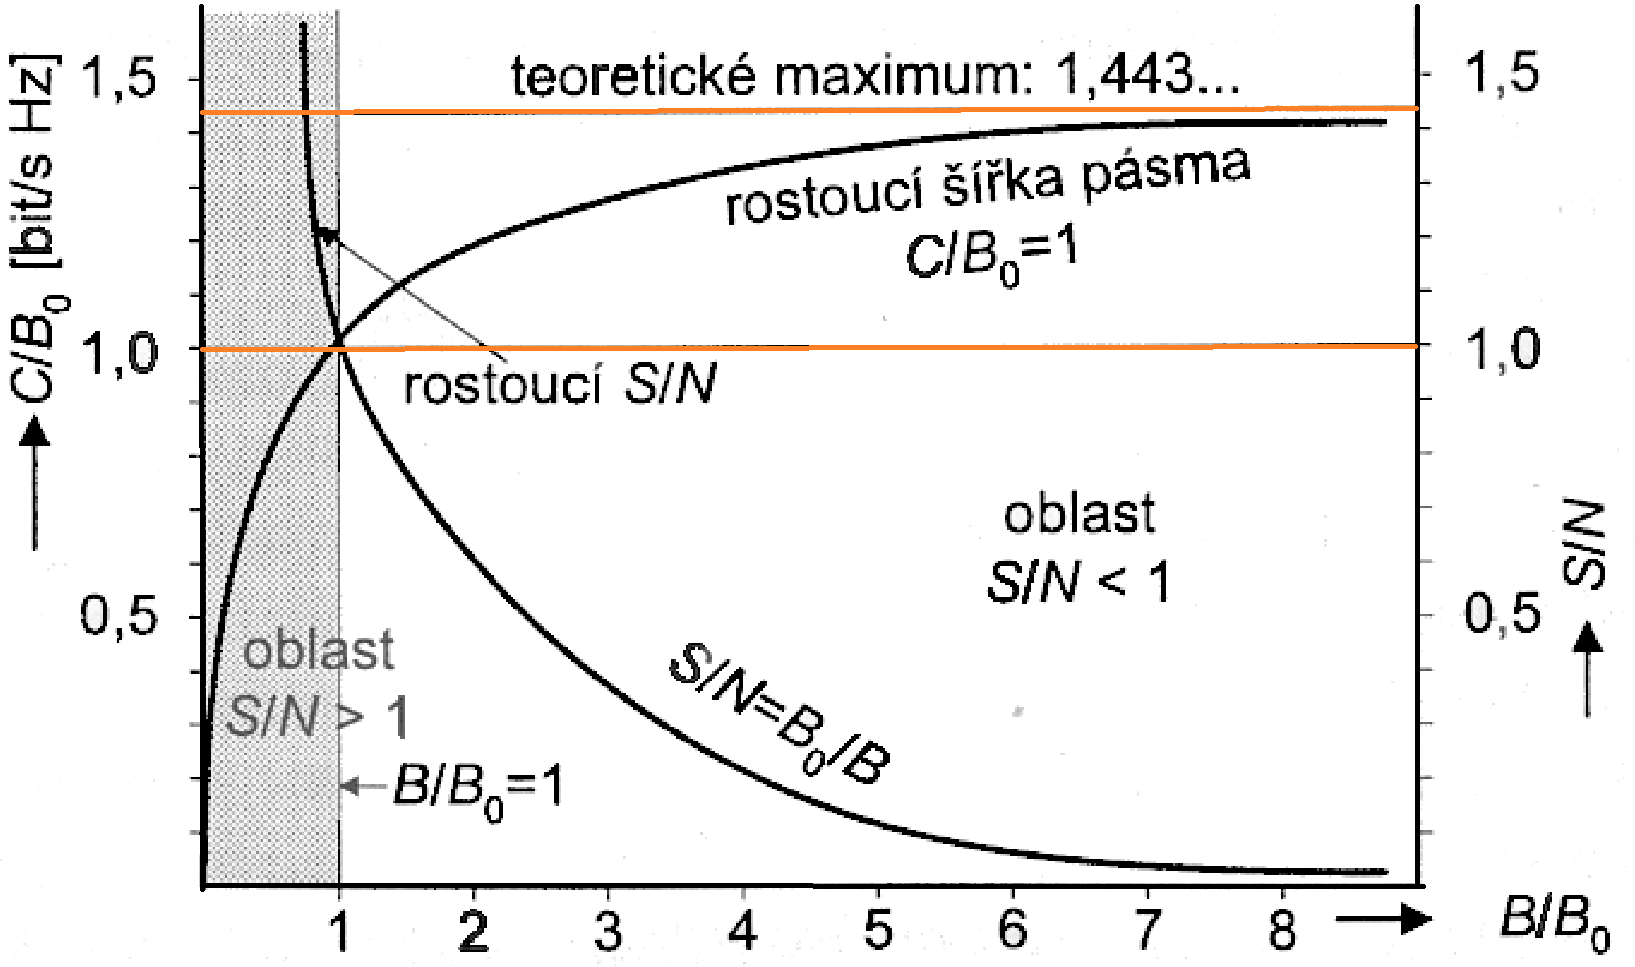
\includegraphics[width=0.8\linewidth]{shannon_graf_C_N.png}
        \caption{Závislost normované přenosové kapacity \(C/B_0\) na poměru signál/šum - \(S/N\)  
                 rádiového komunikačního systému na normované šířce pásma \(B/B_0\)
                  \cite[s.~79]{ZaludRA}}
        \label{fig_RA:modulace02}
      \end{figure} 
      
      Normovaná šířka pásma \(B/B_0\) odpovídá stavu, kdy se výkon signálu \(S\) rovná výkonu šumu 
      \(N\). Svislice vedená bodem \(B/B_0 = 1\) na vodorovné ose potom dělí celý graf na dvě 
      části. Levá, zvýrazněná část odpovídá klasickým radiokomunikačním systémům, které pracují při 
      poměru signál/šum podstatně větším než jedna, přičemž jejich normovaná přenosová kapacita je 
      hluboko pod dosažitelným maximem \(C/B_0 = 1,443\). Pravá část pak odpovídá perspektivním 
      „širokopásmovým“ radiokomunikačním systémům, které naopak pracují při poměru signál/šum \(
      S/N\ll1\), avšak s přenosovou kapacitou blížící se dosažitelnému maximu \(\num{1.443}\). Tyto 
      systémy se označují také jako \textbf{systémy s rozprostřeným spektrem}, nebo \emph{systémy s 
      kódovým multiplexem \texttt{CDMA} (Code Division Multiple Access)}. Jejich realizace je 
      obecně podstatně složitější, než realizace systémů klasických a bez vyspělé monolitické 
      technologie by byla v praxi velmi obtížná. Na druhou stranu však mají systémy druhé kategorie 
      výhodu velice efektivního využití kmitočtového spektra, které totiž mohou sdílet s jinými 
      radiokomunikačními službami aniž by se vzájemně rušily. Mezi jejich další hlavní přednosti 
      náleží možnost dobře pracovat v radiokomunikačních kanálech s vysokou úrovní poruch nebo i 
      úmyslného rušení, dále schopnost účinně potlačovat úniky signálu a konečně i schopnost 
      poměrně spolehlivě utajit přenos před nepovolanými subjekty.\cite[s.~78]{ZaludRA}
     
      
  \section{Modulace a jejich klasifikace}
    V rádiové komunikaci se používá větší počet různých typů (formátů) modulací. Jejich základní 
    klasifikace, vycházející z časového vývoje, je uvedena na obr \ref{fig_RA:modulace03}. Vývojově 
    nejstarší jsou \emph{analogové modulace}. Později se začaly uplatňovat i \emph{diskrétní 
    modulace}, a to nejprve v základním pásmu a potom i v oblasti vysokofrekvenční. Diskrétní 
    modulace v základním pásmu byly nejprve \emph{nekódované}, za nimi potom následovaly i modulace 
    \emph{kódované}. Nejmladší jsou potom \emph{diskrétní modulace s nosnými vlnami}, které pro 
    stručnost dále nazýváme \emph{modulace digitální}. Uveďme si podrobnější klasifikaci všech 
    zmíněných variant. \cite[s.~82]{ZaludRA}
    \begin{figure}[ht!]  % \ref{fig_RA:modulace03}
      \centering
      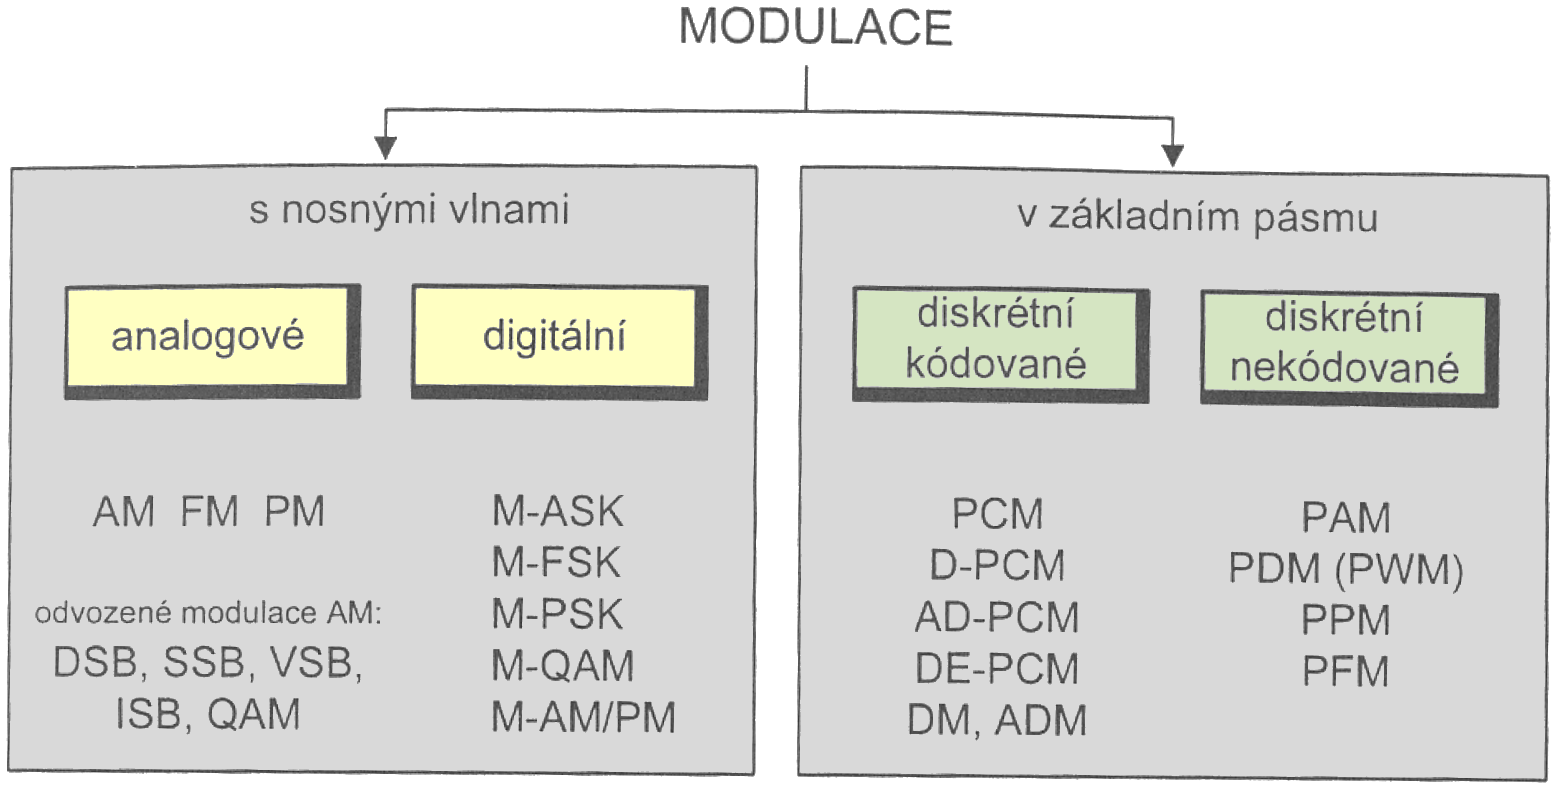
\includegraphics[width=0.9\linewidth]{modulace_prehled.png}
      \caption{Přehled modulačních způsobů používaných v rádiové komunikaci
                \cite[s.~82]{ZaludRA}}
      \label{fig_RA:modulace03}
    \end{figure}
    
    \subsection{Klasifikace analogových modulací}
      Analogové modulace vznikají tak, že se pomocí analogového modulačního signálu (tedy signálu 
      spojitého v čase i v amplitudě) moduluje analogová sinusová vysokofrekvenční nebo mikrovlnná 
      nosná vlna. Modulací se přitom rozumí ovlivňování některého parametru (charakteristické 
      veličiny) nosné vlny modulačním signálem. Je-li to amplituda, vznikne \emph{amplitudová 
      modulace \texttt{AM} (Amplitude Modulation)}, při ovlivňování kmitočtu se vytváří 
      \emph{kmitočtová modulace \texttt{FM} (Frequency Modulation)} a při ovlivňování fáze se 
      vytváří \emph{fázová modulace \texttt{PM} (Phase Modulation)}.
      
      Amplitudově modulovaný signál má kmitočtové spektrum, obsahující nemodulovanou nosnou vlnu a 
      dvě postranní kmitočtová pásma, nesoucí informaci. Určitými modifikacemi tohoto spektra potom 
      vznikají různé vývojově mladší varianty amplitudové modulace \texttt{AM}. 
      \begin{itemize}
        \item \emph{\texttt{AM} s oběma postranními pásmy \texttt{DSB} (Double Side Band)}: jsou 
               přenášena obě postranní pásma, avšak nosná je částečně nebo zcela potlačena,
        \item \emph{\texttt{AM} s jedním potlačeným postranním pásmem \texttt{SSB} (Single Side 
               Band)}: přenos jediného postranního pásma a úplně, nebo alespoň částečně potlačené 
               nosné vlna
        \item \emph{\texttt{AM} s jedním částečně potlačeným postranním pásmem \texttt{VSB} 
               (Vestigial Side Band)}: přenosu jednoho kompletního a jednoho částečně potlačeného 
               postranního pásma. Má obvykle nepotlačenou nosnou vlnu 
        \item \emph{\texttt{AM} s nezávislými postranními pásmy \texttt{ISB} (Independent Side 
               Band)}:Nosná vlna zcela nebo částečně potlačena a v každém úplném postranním pásmu 
               se přenáší nezávislý modulační signál.
        \item \emph{Analogová kvadraturní amplitudová modulace \texttt{QAM} (Quadrature Amplitudě 
               Modulation)}: používá dvě nosné vlny, které mají přesně shodné kmitočty, avšak 
               jejich fázový posuv je trvale \SI{90}{\degreeCelsius}. Každá z těchto nosných vln je 
               amplitudově modulována nezávislým modulačním signálem, přičemž může být částečně 
               nebo zcela potlačena.
      \end{itemize}
      
      Má-li být u předchozích modulací zdůrazněno, že je u nich zcela potlačena nosná vlna, bývá 
      jejich označení ještě doplněno zkratkou \emph{\texttt{SC} (Supressed Carrier)}, tedy 
      například \texttt{DSB-SC}, \texttt{SC-DSB}, nebo \texttt{DSB\textsubscript{SC}}.
      
    \subsection{Diskrétní nekódované modulace v základním pásmu}
      Základním typem této kategorie je \emph{pulzní amplitudová modulace \texttt{PAM} (Pulse 
      Amplitude Modulation)}. Ta vzniká ve své nejjednodušší podobě tak, že se analogový modulační 
      signál přivádí na klíčovaný spínač, který je spínán sledem pravoúhlých impulzů. Za spínačem 
      se potom již objevuje signál \texttt{PAM}, a to v podobě sekvence v čase nespojitých impulzů, 
      jejichž amplitudy kopírují průběh analogového modulačního signálu \cite[s.~84]{ZaludRA}.
      
      Kromě změn amplitudy se u impulzové nosné vlny dají měnit i jiné parametry viz obr. 
      \ref{fig_RA:modulace04}:
      \begin{itemize}
        \item \emph{diskrétní šířková modulace \texttt{PDM}, resp. \texttt{PWM} (Pulse Duration  
              Modulation resp. Pulse Width Modulation)}: změnou šířky impulzů impulzové nosné vlny,
        \item \emph{diskrétní polohová modulace \texttt{PPM} (Pulse Position Modulation)}: změnou  
              polohy impulzů uvažované impulzové nosné vlny, vůči poloze nominální
        \item \emph{diskrétní kmitočtová modulace \texttt{PFM} (Pulse Frequency Modulation)}:  
              změnou kmitočtu této nosné.
      \end{itemize} 
    \subsection{Diskrétní kódované modulace v základním pásmu}
      Nejrozšířenějším typem z této kategorie je \emph{impulzová kódovaná modulace \texttt{PCM} 
      (Pulse Code Modulation)}. Ta se vytváří tak, že se analogový modulační signál nejprve přemění 
      na signál \texttt{PAM}. Ten se poté podrobuje \emph{kvantování}; přitom se jeho celý 
      dynamický rozsah rozdělí na konečný počet \emph{kvantizačních úrovní (hladin)} a každé 
      skutečné úrovni impulzu \texttt{PAM} se přiřadí určitá (například nejbližší) úroveň 
      kvantizační (diskrétní). Kvantovaný signál \texttt{PAM} se dále kóduje. Kódováním se rozumí 
      převod (mapování) jeho skutečné velikosti - vyjádřené obvykle v desítkové soustavě - do 
      soustavy binární (nebo jiné, mající nižší číselný základ, než původní soustava desítková). 
      Tím se vytvoří signál s modulací \texttt{PCM}.
      \begin{itemize}
        \item \emph{diferenční \texttt{D-PCM} (Differentially - \texttt{PCM})}: nekóduje se 
              skutečná velikost kvantovaných vzorků PAM, nýbrž pouze rozdíl mezi touto skutečnou 
              velikostí a velikostí predikovanou (tj. předpověděnou z několika předchozích 
              kvantovaných vzorků).
        \item \emph{diferenciálně kódované \texttt{DE-PCM} (Differentially encoded -
              \texttt{PCM})}: nejprve se vytváří signál \texttt{PCM}; z něho se potom pomocí 
              vhodného algoritmu získává signál \texttt{DE-PCM}, u něhož je informace obsažena 
              nikoliv v samotné logické hodnotě příslušného bitu signálu \texttt{PCM}, nýbrž v 
              rozdílu tohoto bitu oproti hodnotě bitu předchozího.
        \item \emph{delta modulace \texttt{DM} (Delta Modulation)}: v podstatě představuje   
              jednobitovou variantu modulace \texttt{PCM}; je-li \(w\)-tý vzorek analogového 
              modulačního signálu větší než vzorek předchozí, je v signálu \texttt{DM} bit \(1\) a 
              je-li tento vzorek menší než předchozí, je v signálu \texttt{DM} bit \(0\).
      \end{itemize}
      
      Všechny předchozí varianty diskrétních kódovaných modulací pracují s konstantním kvantizačním 
      krokem. U \emph{adaptivní modulace \texttt{D-PCM} tj. \texttt{AD-PCM}} a rovněž u 
      \emph{adaptivní modulace \texttt{DM} tj. \texttt{A-DM}}, se kvantizační krok naopak mění v 
      závislosti na průběhu analogového modulačního signálu.
    
    \begin{figure}[ht!]  % \ref{fig_RA:modulace04}
      \centering
      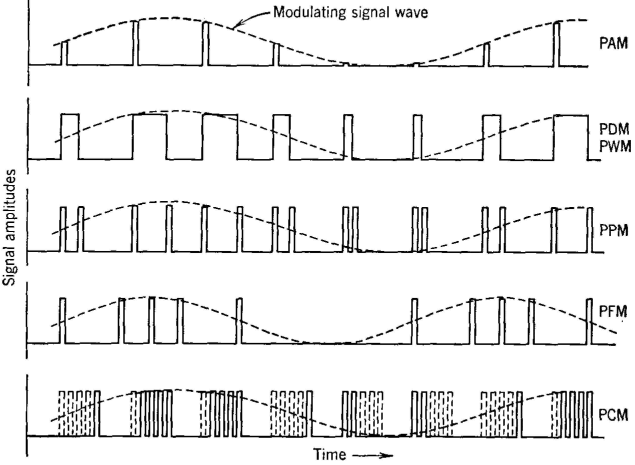
\includegraphics[width=1\linewidth]{modulace_zakladni_pasmo.png}
      \caption{Přibližné tvary a uspořádání signálů diskrétních pulsní modulací pro sinusový   
               modulační signál (tečkovaná křivka). Výška impulsů obecně neodpovídá výšce modulační 
               vlny.}
      \label{fig_RA:modulace04}
    \end{figure}
    
    \subsection{Digitální modulace (diskrétní modulace s nosnými vlnami)}
      Tyto modulace vznikají tak, že se vysokofrekvenční nebo mikrovlnná sinusová nosná vlna 
      moduluje signálem některé diskrétní modulace v základním pásmu; jedná se zde tedy vlastně o 
      dvojnásobnou modulaci, neboť modulačním signálem je již předtím modulovaný signál. K modulaci 
      se používá většinou binární signál \texttt{PCM}, nebo jeho některé modifikace, ostatní 
      diskrétní modulace se k danému účelu používají jen zřídka.
      
      Binárním modulačním signálem je možné modulovat amplitudu, kmitočet anebo fázi nosné vlny. U 
      \emph{dvoustavových modulací} se modulovaný parametr této vlny mění pouze mezi dvěma 
      diskrétními stavy, z nichž jeden odpovídá modulačnímu bitu 0 a druhý bitu 1. Tyto diskrétní 
      stavy nosné vlny se u digitálních modulací označují obecně termínem \emph{signálové prvky} 
      resp. \emph{symboly}, okamžiky přechodu mezi nimi se potom nazývají \emph{charakteristické 
      okamžiky}. Pro uvažované digitální modulace se používá rovněž termín \textbf{klíčování}; 
      (změny nosné vlny mezi několika diskrétními stavy se tímto slovem označují vlastně již od 
      počátků radiokomunikace, nejprve zřejmě ve spojení „klíčovaná telegrafie“).
      \begin{itemize}
        \item \emph{dvoustavové klíčování amplitudovým zdvihem \texttt{2-ASK} (Amplitudě Shift  
              Keying)}: klíčováním amplitudy nosné vlny, se získá dvoustavová modulace 
              \texttt{PCM-AM}
        \item \emph{dvoustavové klíčování kmitočtovým zdvihem \texttt{2-FSK} (Frequency Shift  
              Keying)}: klíčování kmitočtu nosné vlny se vytváří dvoustavová modulace 
              \texttt{PCM-FM},
        \item \emph{dvoustavové klíčování fázovým zdvihem \texttt{2-PSK}, (Phase Shift Keying)}: 
              klíčování fáze nosné vlny potom konečně vzniká dvoustavová modulace \texttt{PCM-PM}.
      \end{itemize}
      U dvoustavových modulací odpovídá každý modulační stav modulované nosné vlny jedinému bitu 
      modulačního signálu \texttt{PCM}. Snaha po zvětšení přenosové kapacity digitálních modulací 
      však vedla k rychlému rozvoji \emph{vícestavových diskrétních modulací}, u nichž každý 
      signálový prvek modulované nosné vlny přenáší nejméně dva, nebo i více bitů. Tak například u 
      \emph{čtyřstavové modulace \texttt{4-FSK (Q-FSK)}} tato vlna zaujímá čtyři diskrétní 
      kmitočty; každá z nich zde však již nereprezentuje jediný bit jako v případě modulace 
      \texttt{2-FSK}, nýbrž dva bity, tj. \emph{bitovou dvojici}, nazývanou také \emph{dibit}. 
      Analogicky   \emph{čtyřstavová modulace \texttt{4-PSK (Q-PSK)}} pracuje se čtyřmi diskrétními 
      fázovými 
      stavy nosné vlny, z nichž každý odpovídá určitému dibitu modulačního signálu atd. Rychlost, 
      se kterou se mění diskrétní stavy nosné vlny se nazývá \textbf{symbolová rychlost} \(f_s\) 
      tato rychlost se vyjadřuje v jednotkách \emph{baud \textbf{[Bd]}}, přičemž je rovna reciproké 
      hodnotě doby trvání \(T_s\) signálového prvku, tedy\[f_s = \frac{1}{T_s}.\]
      
      U čtyřstavových modulací \texttt{4-ASK}, \texttt{4-FSK} a \texttt{4-PSK} zřejmě každý 
      signálový prvek přenáší dva bity, proto je zde symbolová rychlost \(f_s\) rovna právě jedné 
      polovině bitové rychlosti \(f_b\) V důsledku toho je potom i potřebná šířka pásma 
      vy\-so\-ko\-frek\-ven\-ční\-ho kanálu u těchto modulací poloviční, v porovnání s modulacemi 
      dvoustavovými (ovšem při téže bitové rychlosti modulačního signálu \texttt{PCM}). U 
      osmistavových modulací nese každý signálový prvek informaci již o třech bitech (tj. o jednom 
      \textbf{tribitu}), což vede pouze ke třetinové šířce pásma vysokofrekvenčního kanálu. Obecně 
      potom platí, že u modulace s \(M\) stavy přenáší každý symbol informaci o \(n = \log_2 M\) 
      bitech. Šířka pásma \(B_M\) kanálu obecné \emph{M-stavové modulace}, v závislosti na šířce 
      pásma \(B_2\) základní dvoustavové modulace, je tedy určena vztahem \(B_M = \frac{B_2}{\log_2 
      M}.\) 
      
      Vývojově mladší kategorii digitálních modulací potom představují \emph{M-stavové modulace se 
      současným klíčováním amplitudy a fáze nosné vlny}, značené původně symbolem 
      \texttt{M-ASK/PSK}; pro tyto modulace je však již běžnější označení \emph{M-stavové 
      kvadraturní amplitudové modulace \texttt{M-QAM}\footnote{nezaměňovat s analogovou kvadraturní 
      modulací \texttt{QAM}, popisovanou výše} (Quadrature Amplitude Modulation)}.
      
      Od počátku devadesátých let se dostávají do praxe také již zmíněné \emph{kódované modulace}, 
      které vznikají spojením kanálového kódování a vlastní modulace do jediného procesu, 
      realizovaného v jediném funkčním bloku. 
    
    \subsection{Lineární modulace a nelineární modulace, modulace s pamětí a bez paměti}
      Předchozí klasifikace modulací vychází z jejich historického vývoje, přičemž rozlišuje 
      jednotlivé modulace na základě různých typů modulačních signálů a rozdílných modulovaných 
      parametrů nosné vlny.
      
      Dělení na \textbf{lineární} a \textbf{nelineární modulace} se uplatňuje především u modulací 
      s nosnými vlnami. \emph{Analogové lineární modulace} jsou takové, u nichž je amplituda nosné 
      vlny danou, obecně lineární funkcí okamžitých hodnot modulačního signálu. U lineárních 
      modulací Platí \emph{princip superpozice} mezi různými složkami kmitočtového spektra 
      modulovaného signálu, příslušejícími různým složkám spektra modulačního signálu. Do této 
      kategorie patří amplitudová modulace AM i všechny její varianty, tj. modulace \texttt{DSB}, 
      \texttt{SSD} atd. U \emph{analogových nelineárních modulací} zmíněná lineární závislost 
      amplitudy nosné na modulačním signálu neexistuje a princip superpozice neplatí, takže ve 
      spektru modulovaného 
      signálu jsou přítomny také \emph{intermodulační produkty} základních složek. Sem náležejí dvě 
      kategorie tzv. \emph{exponenciálních modulací}, a to \emph{kmitočtová modulace \texttt{FM}} a 
      \emph{fázová modulace \texttt{PM}}; tyto modulace jsou charakterizovány \emph{konstantní 
      obálkou nosné vlny}. U \emph{diskrétních lineárních modulací} při mapování modulačního 
      digitálního signálu (informační datové sekvence), do po sobě následujících stavů (signálových 
      prvků) modulované nosné vlny, platí princip superpozice. U \emph{diskrétních nelineárních 
      modulací} naopak princip superpozice mezi po sobě následujícími stavy modulovaného signálu 
      neplatí. Tyto   modulace mohou, ale také nemusí mít konstantní obálkou modulované nosné vlny, 
      v závislosti na tom zda se u nich netvaruje - nebo tvaruje modulační datová sekvence.
      
      U \textbf{digitálních modulací s pamětí} určitý stav nosné vlny závisí nejen na jemu 
      odpovídajícím bloku (kódové skupině) binárního modulačního signálu, nýbrž určitým způsobem i 
      na předchozích stavech této vlny, resp. na předchozích blocích modulačního signálu. Uvedená 
      závislost zde vzniká zpravidla již na úrovni modulačních signálů, které se totiž z původní 
      vstupní podoby nejprve překódují do podoby „s pamětí“ a teprve poté se přivádějí na 
      modulátor. U \textbf{digitálních modulací bez paměti} se tato závislost neobjevuje.
      
      Výše uvedené kategorie se mohou vzájemně kombinovat, čímž vznikají celkem čtyři možné 
      varianty, které se striktně rozlišují především u digitálních modulací. K lineárním modulacím 
      bez paměti náležejí například formáty \texttt{2-PSK, 4-PSK,} k lineárním modulacím s pamětí 
      formáty \texttt{DE-PSK, \(\pi\)/4-QPSK} atd. 
      
      Poslední klasifikace se týká pouze modulací, u nichž je modulační signál \emph{nespojitý 
      (diskrétní) v čase}. \textbf{Koherentní modulace} jsou takové, u nichž existuje předem určený 
      vztah mezi okamžiky charakterizujícími fázi nosné vlny před modulací a charakteristickými 
      okamžiky modulovaného signálu. Do této kategorie náležejí například modulace, u nichž 
      charakteristické okamžiky modulovaného signálu splývají s průchody nosné vlny nulou 
      (konkrétně je to např. modulace MSK apod.). Modulace, u nichž předem určený vztah mezi fází 
      nosné vlny a charakteristickými okamžiky modulovaného signálu neexistuje, se nazývají 
      \textbf{modulace nekoherentní}.
      
  \section{Analogové modulace}
    Vývojově nejstarší systémy pro pozemskou radiokomunikaci používaly pro přenos analogovou 
    amplitudovou modulaci \texttt{AM}, k níž se později připojila analogová kmitočtová modulace 
    \texttt{FM} a fázová modulace \texttt{PM}. Modulace \texttt{AM} a její varianty se v současné 
    době uplatňují spíše už jen u jednodušších systémů, jako je například rozhlas \texttt{AM}, 
    občanské radiostanice apod. Naproti tomu modulace \texttt{FM} stále ještě nachází využití i v 
    náročnějších aplikacích jako je stereofonní rozhlas \texttt{FM} apod \cite[s.~75]{ZaludRA}.
    
    \subsection{Základní principy analogových modulací}
      U analogových modulací se obecným modulačním signálem \(m(t)\) moduluje vhodný parametr 
      spojité, harmonické (např. kosinusové) vysokofrekvenční nosné vlny. Modulační signál může mít 
      charakter napětí nebo proudu, v dalším však většinou předpokládáme, že je to signál napěťový. 
      Modulované napětí lze potom vyjádřit obecným vztahem
      \begin{equation}\label{eq:RA_mdlc_01}
        u_{mod}(t) = u_i(t)\cos[\Phi_i(t)]
      \end{equation}
      kde \(u_i (t)\) je \emph{okamžitá amplituda} napětí modulované nosné vlny; \(\Phi_i(t)\) 
      okamžitá fáze modulované nosné vlny.
      
      Mění-li se amplituda napětí \(u_i(t)\) modulované nosné vlny lineárně s modulačním napětím 
      \(m(t)\), přičemž okamžitá fáze \(\Phi_i(t)\) zůstává konstantní, získá se \emph{amplitudová 
      modulace}, která náleží do kategorie \emph{lineárních modulací}. U lineárních modulací jsou v 
      kmitočtovém spektru modulovaného signálu obsaženy jen složky, které odpovídají jednotlivým 
      harmonickým složkám modulačního signálu.
      
      Jestliže se u modulované nosné vlny mění podle určitého zákona okamžitá fáze \(\Phi_i(t)\) s 
      modulačním napětím \(m(t)\), přičemž amplituda zůstává konstantní, vytvářejí se \emph{úhlové 
      (exponenciální) modulace}, náležející do kategorie \emph{nelineárních modulací}. V jejich 
      kmitočtovém spektru jsou nejen složky odpovídající jednotlivým harmonickým modulačního 
      signálu, nýbrž i jejich vzájemné intermodulační produkty. Z nich je nejčastěji využívána 
      \emph{kmitočtová modulace \texttt{FM}}, u níž je okamžitá odchylka kmitočtu (tj. derivace 
      fáze podle času) modulované nosné vlny, vůči kmitočtu nemodulované nosné vlny, úměrná 
      modulačnímu signálu. K exponenciálním modulacím náleží dále \emph{fázová modulace 
      \texttt{PM}}, u níž je okamžitá odchylka fáze, od fáze nemodulované nosné vlny, úměrná 
      modulačnímu signálu. Modulace \texttt{FM} a \texttt{PM} mají konstantní obálku modulované 
      nosné vlny. To je v praxi výhodné, neboť signály s konstantní obálkou mohou být zesilovány 
      výkonovými zesilovači nastavenými do nelineární pracovní třídy C (D, E, ...), vyznačující se 
      velkou energetickou účinností, okolo \num{50} až \num{80}\%.
      
    \subsection{Amplitudová modulace AM}
      Základním typem amplitudových modulací je \emph{amplitudová modulace s oběma postranními 
      pásmy a nepotlačenou nosnou vlnou}, značená symbolem \emph{\texttt{AM} (Amplitude 
      Modulation)}. Její podstatu ukazuje obr. \ref{fig_RA:modulace05}. Na obr. 
      \ref{fig_RA:modulace06} je znázorněn časový průběh modulačního signálu \(m(t)\), o němž 
      nejprve pro jednoduchost předpokládejme, že je kosinusový (harmonický) a má amplitudu 
      \(U_m\) a kmitočet \(f_m\). Na obr. \ref{fig_RA:modulace07} je znázorněna kosinusová nosná 
      vlna \(u_c(t)\) o amplitudě \(Uc\) a kmitočtu \(f_c\). Tyto průběhy lze vyjádřit relacemi
      \begin{equation}\label{eq:RA_mdlc_02}
        m(t) = U_m(t)\cos(2\pi f_m t); \qquad u_c(t) = U_c(t)\cos(2\pi f_c t)
      \end{equation}

      \begin{figure}[ht!]
        \centering
        \subcaptionbox{harmonický (kosinusový) modulační signál \(m(t)\) \label{fig_RA:modulace05}}
          {\luafigure[0.8]{modulace05_AM.png}}              \newline
        \subcaptionbox{harmonická (kosinusová) nosná vlna \(u_c(t)\)     \label{fig_RA:modulace06}}
         {\luafigure[0.8]{modulace06_AM.png}}              \newline
        \subcaptionbox{odpovídající modulovaný \texttt{AM} signál  
                  \(u_{AM}(t)\)                                          \label{fig_RA:modulace07}}
          {\luafigure[0.8]{modulace07_AM.png}}              \newline
        \subcaptionbox{kmitočtové spektrum \(F_{AM}(f)\) signálu AM při obecném, neharmonickém  
                  modulačním signálu                                     \label{fig_RA:modulace08}}
          {\luafigure[0.7]{modulace08_AM.png}}              \newline
        \subcaptionbox{fázorová reprezentace signálu \texttt{AM}.        \label{fig_RA:modulace09}}
          {\luafigure[0.7]{modulace09_AM.png}}  
        \caption{Podstata amplitudové modulace \texttt{AM}}
      \end{figure}
      
      Amplitudová modulace \texttt{AM} je definována jako modulace, při níž se amplituda nosné vlny 
      mění okolo své střední hodnoty \(U_c\) lineárně s modulačním signálem \(m(t)\). Časový průběh 
      příslušného modulovaného napětí \(u_m(t)\), znázorněného na obr. \ref{fig_RA:modulace07} je 
      tedy dán relací
    
%--------------------------------------------------------------------------------------------------- 
} % DEBUG was off

\printbibliography[title={Seznam literatury}, heading=bibliography]